\documentclass[twoside]{book}

% Packages required by doxygen
\usepackage{fixltx2e}
\usepackage{calc}
\usepackage{doxygen}
\usepackage[export]{adjustbox} % also loads graphicx
\usepackage{graphicx}
\usepackage[utf8]{inputenc}
\usepackage{makeidx}
\usepackage{multicol}
\usepackage{multirow}
\PassOptionsToPackage{warn}{textcomp}
\usepackage{textcomp}
\usepackage[nointegrals]{wasysym}
\usepackage[table]{xcolor}

% Font selection
\usepackage[T1]{fontenc}
\usepackage[scaled=.90]{helvet}
\usepackage{courier}
\usepackage{amssymb}
\usepackage{sectsty}
\renewcommand{\familydefault}{\sfdefault}
\allsectionsfont{%
  \fontseries{bc}\selectfont%
  \color{darkgray}%
}
\renewcommand{\DoxyLabelFont}{%
  \fontseries{bc}\selectfont%
  \color{darkgray}%
}
\newcommand{\+}{\discretionary{\mbox{\scriptsize$\hookleftarrow$}}{}{}}

% Page & text layout
\usepackage{geometry}
\geometry{%
  a4paper,%
  top=2.5cm,%
  bottom=2.5cm,%
  left=2.5cm,%
  right=2.5cm%
}
\tolerance=750
\hfuzz=15pt
\hbadness=750
\setlength{\emergencystretch}{15pt}
\setlength{\parindent}{0cm}
\setlength{\parskip}{3ex plus 2ex minus 2ex}
\makeatletter
\renewcommand{\paragraph}{%
  \@startsection{paragraph}{4}{0ex}{-1.0ex}{1.0ex}{%
    \normalfont\normalsize\bfseries\SS@parafont%
  }%
}
\renewcommand{\subparagraph}{%
  \@startsection{subparagraph}{5}{0ex}{-1.0ex}{1.0ex}{%
    \normalfont\normalsize\bfseries\SS@subparafont%
  }%
}
\makeatother

% Headers & footers
\usepackage{fancyhdr}
\pagestyle{fancyplain}
\fancyhead[LE]{\fancyplain{}{\bfseries\thepage}}
\fancyhead[CE]{\fancyplain{}{}}
\fancyhead[RE]{\fancyplain{}{\bfseries\leftmark}}
\fancyhead[LO]{\fancyplain{}{\bfseries\rightmark}}
\fancyhead[CO]{\fancyplain{}{}}
\fancyhead[RO]{\fancyplain{}{\bfseries\thepage}}
\fancyfoot[LE]{\fancyplain{}{}}
\fancyfoot[CE]{\fancyplain{}{}}
\fancyfoot[RE]{\fancyplain{}{\bfseries\scriptsize Generated by Doxygen }}
\fancyfoot[LO]{\fancyplain{}{\bfseries\scriptsize Generated by Doxygen }}
\fancyfoot[CO]{\fancyplain{}{}}
\fancyfoot[RO]{\fancyplain{}{}}
\renewcommand{\footrulewidth}{0.4pt}
\renewcommand{\chaptermark}[1]{%
  \markboth{#1}{}%
}
\renewcommand{\sectionmark}[1]{%
  \markright{\thesection\ #1}%
}

% Indices & bibliography
\usepackage{natbib}
\usepackage[titles]{tocloft}
\setcounter{tocdepth}{3}
\setcounter{secnumdepth}{5}
\makeindex

% Hyperlinks (required, but should be loaded last)
\usepackage{ifpdf}
\ifpdf
  \usepackage[pdftex,pagebackref=true]{hyperref}
\else
  \usepackage[ps2pdf,pagebackref=true]{hyperref}
\fi
\hypersetup{%
  colorlinks=true,%
  linkcolor=blue,%
  citecolor=blue,%
  unicode%
}

% Custom commands
\newcommand{\clearemptydoublepage}{%
  \newpage{\pagestyle{empty}\cleardoublepage}%
}

\usepackage{caption}
\captionsetup{labelsep=space,justification=centering,font={bf},singlelinecheck=off,skip=4pt,position=top}

%===== C O N T E N T S =====

\begin{document}

% Titlepage & ToC
\hypersetup{pageanchor=false,
             bookmarksnumbered=true,
             pdfencoding=unicode
            }
\pagenumbering{roman}
\begin{titlepage}
\vspace*{7cm}
\begin{center}%
{\Large Reference Manual\\[1ex]\large beta }\\
\vspace*{1cm}
{\large Generated by Doxygen 1.8.11}\\
\end{center}
\end{titlepage}
\clearemptydoublepage
\tableofcontents
\clearemptydoublepage
\pagenumbering{arabic}
\hypersetup{pageanchor=true}

%--- Begin generated contents ---
\chapter{Documentation for T\+H\+E\+M\+IS}
\label{index}\hypertarget{index}{}This is the documentation for the source code in T\+H\+E\+M\+IS.



The documentation is divided in the following sections\+:
\begin{DoxyItemize}
\item \hyperlink{intro}{Introduction}
\item \hyperlink{conv}{Coding Conventions} 
\end{DoxyItemize}
\chapter{Introduction}
\label{intro}
\hypertarget{intro}{}
T\+H\+E\+M\+IS is a program to study intermolecular recognition via direct partition function estimation.~

Currently T\+H\+E\+M\+IS is developed in the \href{http://www.lqt.dq.ufscar.br}{\tt Theoretical Chemistry Laboratory} 
\chapter{Coding Conventions}
\label{conv}
\hypertarget{conv}{}
On this page we describe the coding conventions that should be used when adding or changing T\+H\+E\+M\+IS code.\hypertarget{conv_themis}{}\section{T\+H\+E\+M\+IS}\label{conv_themis}
In this section we give a short introduction to T\+H\+E\+M\+IS. We explain the basic usage and show how an automatic documentation of the code can be achieved. To this end one has to add special markers to the comments in the code. This can be done on the fly with little additional work.\hypertarget{conv_code}{}\subsection{Code Documentation}\label{conv_code}
\hypertarget{conv_basic}{}\subsubsection{Basics}\label{conv_basic}
\+\_\+\+\_\+\+\_\+ \begin{DoxyVerb}/*!
 * ... THEMIS  ....
 */ 
subroutine read_input()
{ ..... }
\end{DoxyVerb}


\begin{DoxyVerb} function calc()
\end{DoxyVerb}


\begin{DoxyVerb}/*! \brief A short description of the function 
 *
 */ 
\end{DoxyVerb}
\hypertarget{conv_theory}{}\subsubsection{Theory}\label{conv_theory}




T\+H\+E\+M\+IS ... Partition function\+:~

$ Z = \frac{1}{h^{3}}\int exp(-\beta H(q,p))d^{3}qd^{3}p $.. 
\chapter{Namespace Index}
\section{Namespace List}
Here is a list of all namespaces with brief descriptions\+:\begin{DoxyCompactList}
\item\contentsline{section}{\hyperlink{namespacemod__cmd__line}{mod\+\_\+cmd\+\_\+line} \\*This module contains a routine to get command line arguments }{\pageref{namespacemod__cmd__line}}{}
\item\contentsline{section}{\hyperlink{namespacemod__constants}{mod\+\_\+constants} \\*This module defines a set constants }{\pageref{namespacemod__constants}}{}
\item\contentsline{section}{\hyperlink{namespacemod__deallocate__all}{mod\+\_\+deallocate\+\_\+all} \\*This module constains instructions to deallocate all arrays prior to program termination }{\pageref{namespacemod__deallocate__all}}{}
\item\contentsline{section}{\hyperlink{namespacemod__input__read}{mod\+\_\+input\+\_\+read} \\*This module contains a routine for I\+N\+P\+UT reading and checking }{\pageref{namespacemod__input__read}}{}
\item\contentsline{section}{\hyperlink{namespacemod__inquire}{mod\+\_\+inquire} \\*This module performs inquire checks for all files that will be read }{\pageref{namespacemod__inquire}}{}
\item\contentsline{section}{\hyperlink{namespacemod__loops}{mod\+\_\+loops} \\*This module contains the main program loop for Z(\+N,\+V,\+T) calculation }{\pageref{namespacemod__loops}}{}
\item\contentsline{section}{\hyperlink{namespacemod__pot__ljc}{mod\+\_\+pot\+\_\+ljc} \\*This module performs LJ + coulombic potential calculations }{\pageref{namespacemod__pot__ljc}}{}
\item\contentsline{section}{\hyperlink{namespacemod__pot__none}{mod\+\_\+pot\+\_\+none} \\*This module performs interatomic distance calculations when no potential is selected }{\pageref{namespacemod__pot__none}}{}
\item\contentsline{section}{\hyperlink{namespacemod__read__grids}{mod\+\_\+read\+\_\+grids} \\*This module reads coordinate files for translation and rotation grids }{\pageref{namespacemod__read__grids}}{}
\item\contentsline{section}{\hyperlink{namespacemod__read__xyz}{mod\+\_\+read\+\_\+xyz} \\*This module reads coordinate files for xyz\+\_\+files 1 and 2 }{\pageref{namespacemod__read__xyz}}{}
\item\contentsline{section}{\hyperlink{namespacemod__resume}{mod\+\_\+resume} \\*This module contains routines that resume the run }{\pageref{namespacemod__resume}}{}
\item\contentsline{section}{\hyperlink{namespacemod__search}{mod\+\_\+search} \\*This module contains routines to search and write the lowest energy structures for the run }{\pageref{namespacemod__search}}{}
\item\contentsline{section}{\hyperlink{namespacemod__spherical__grids}{mod\+\_\+spherical\+\_\+grids} }{\pageref{namespacemod__spherical__grids}}{}
\item\contentsline{section}{\hyperlink{namespacemod__vmd}{mod\+\_\+vmd} \\*This module contains instructions to write V\+MD scripts for visualization of properties around central grid }{\pageref{namespacemod__vmd}}{}
\item\contentsline{section}{\hyperlink{namespacexdr}{xdr} \\*X\+DR Fortran Interface with Wrappers }{\pageref{namespacexdr}}{}
\end{DoxyCompactList}

\chapter{Hierarchical Index}
\section{Class Hierarchy}
This inheritance list is sorted roughly, but not completely, alphabetically\+:\begin{DoxyCompactList}
\item \contentsline{section}{mod\+\_\+read\+\_\+molecules\+:\+:atom}{\pageref{structmod__read__molecules_1_1atom}}{}
\item atom\begin{DoxyCompactList}
\item \contentsline{section}{mod\+\_\+pot\+\_\+bhc\+:\+:bhc\+\_\+atom}{\pageref{structmod__pot__bhc_1_1bhc__atom}}{}
\end{DoxyCompactList}
\item dimer\begin{DoxyCompactList}
\item \contentsline{section}{mod\+\_\+pot\+\_\+bhc\+:\+:bhc\+\_\+dimer}{\pageref{structmod__pot__bhc_1_1bhc__dimer}}{}
\item \contentsline{section}{mod\+\_\+pot\+\_\+ljc\+:\+:ljc\+\_\+dimer}{\pageref{structmod__pot__ljc_1_1ljc__dimer}}{}
\end{DoxyCompactList}
\item \contentsline{section}{mod\+\_\+read\+\_\+molecules\+:\+:dimer}{\pageref{structmod__read__molecules_1_1dimer}}{}
\begin{DoxyCompactList}
\item \contentsline{section}{mod\+\_\+pot\+\_\+ljc\+\_\+pair\+:\+:ljc\+\_\+pair\+\_\+dimer}{\pageref{structmod__pot__ljc__pair_1_1ljc__pair__dimer}}{}
\end{DoxyCompactList}
\item \contentsline{section}{mod\+\_\+error\+\_\+handling\+:\+:error}{\pageref{structmod__error__handling_1_1error}}{}
\item \contentsline{section}{mod\+\_\+read\+\_\+grids\+:\+:grid}{\pageref{structmod__read__grids_1_1grid}}{}
\item molecule\begin{DoxyCompactList}
\item \contentsline{section}{mod\+\_\+pot\+\_\+bhc\+:\+:bhc\+\_\+molecule}{\pageref{structmod__pot__bhc_1_1bhc__molecule}}{}
\end{DoxyCompactList}
\item \contentsline{section}{mod\+\_\+read\+\_\+molecules\+:\+:molecule}{\pageref{structmod__read__molecules_1_1molecule}}{}
\item \contentsline{section}{mod\+\_\+read\+\_\+grids\+:\+:point}{\pageref{structmod__read__grids_1_1point}}{}
\item \contentsline{section}{mod\+\_\+vmd\+:\+:W\+R\+I\+T\+E\+\_\+\+V\+M\+D\+\_\+\+F\+I\+L\+ES}{\pageref{interfacemod__vmd_1_1WRITE__VMD__FILES}}{}
\item \contentsline{section}{xdr\+:\+:xtcfile}{\pageref{structxdr_1_1xtcfile}}{}
\end{DoxyCompactList}

\chapter{Class Index}
\section{Class List}
Here are the classes, structs, unions and interfaces with brief descriptions\+:\begin{DoxyCompactList}
\item\contentsline{section}{\hyperlink{structmod__pot__ljc_1_1dimer__ljc}{mod\+\_\+pot\+\_\+ljc\+::dimer\+\_\+ljc} }{\pageref{structmod__pot__ljc_1_1dimer__ljc}}{}
\item\contentsline{section}{\hyperlink{structmod__read__grids_1_1grid}{mod\+\_\+read\+\_\+grids\+::grid} }{\pageref{structmod__read__grids_1_1grid}}{}
\item\contentsline{section}{\hyperlink{structmod__pot__ljc_1_1ljc__atom}{mod\+\_\+pot\+\_\+ljc\+::ljc\+\_\+atom} }{\pageref{structmod__pot__ljc_1_1ljc__atom}}{}
\item\contentsline{section}{\hyperlink{structmod__pot__ljc_1_1ljc__mol}{mod\+\_\+pot\+\_\+ljc\+::ljc\+\_\+mol} }{\pageref{structmod__pot__ljc_1_1ljc__mol}}{}
\item\contentsline{section}{\hyperlink{structmod__read__grids_1_1point}{mod\+\_\+read\+\_\+grids\+::point} }{\pageref{structmod__read__grids_1_1point}}{}
\item\contentsline{section}{\hyperlink{structmod__read__xyz_1_1point}{mod\+\_\+read\+\_\+xyz\+::point} }{\pageref{structmod__read__xyz_1_1point}}{}
\item\contentsline{section}{\hyperlink{structxdr_1_1xtcfile}{xdr\+::xtcfile} }{\pageref{structxdr_1_1xtcfile}}{}
\item\contentsline{section}{\hyperlink{structmod__read__xyz_1_1xyz__dimer}{mod\+\_\+read\+\_\+xyz\+::xyz\+\_\+dimer} }{\pageref{structmod__read__xyz_1_1xyz__dimer}}{}
\item\contentsline{section}{\hyperlink{structmod__read__xyz_1_1xyz__file}{mod\+\_\+read\+\_\+xyz\+::xyz\+\_\+file} }{\pageref{structmod__read__xyz_1_1xyz__file}}{}
\end{DoxyCompactList}

\chapter{File Index}
\section{File List}
Here is a list of all files with brief descriptions\+:\begin{DoxyCompactList}
\item\contentsline{section}{/home/alozada/\+T\+H\+E\+M\+I\+S\+\_\+\+D\+E\+C\+E\+M\+B\+E\+R/themis-\/dev\+\_\+december/code/src/\hyperlink{mod__cmd__line_8f90}{mod\+\_\+cmd\+\_\+line.\+f90} }{\pageref{mod__cmd__line_8f90}}{}
\item\contentsline{section}{/home/alozada/\+T\+H\+E\+M\+I\+S\+\_\+\+D\+E\+C\+E\+M\+B\+E\+R/themis-\/dev\+\_\+december/code/src/\hyperlink{mod__constants_8f90}{mod\+\_\+constants.\+f90} }{\pageref{mod__constants_8f90}}{}
\item\contentsline{section}{/home/alozada/\+T\+H\+E\+M\+I\+S\+\_\+\+D\+E\+C\+E\+M\+B\+E\+R/themis-\/dev\+\_\+december/code/src/\hyperlink{mod__deallocate__all_8f90}{mod\+\_\+deallocate\+\_\+all.\+f90} }{\pageref{mod__deallocate__all_8f90}}{}
\item\contentsline{section}{/home/alozada/\+T\+H\+E\+M\+I\+S\+\_\+\+D\+E\+C\+E\+M\+B\+E\+R/themis-\/dev\+\_\+december/code/src/\hyperlink{mod__error__handling_8f90}{mod\+\_\+error\+\_\+handling.\+f90} }{\pageref{mod__error__handling_8f90}}{}
\item\contentsline{section}{/home/alozada/\+T\+H\+E\+M\+I\+S\+\_\+\+D\+E\+C\+E\+M\+B\+E\+R/themis-\/dev\+\_\+december/code/src/\hyperlink{mod__info_8f90}{mod\+\_\+info.\+f90} }{\pageref{mod__info_8f90}}{}
\item\contentsline{section}{/home/alozada/\+T\+H\+E\+M\+I\+S\+\_\+\+D\+E\+C\+E\+M\+B\+E\+R/themis-\/dev\+\_\+december/code/src/\hyperlink{mod__input__read_8f90}{mod\+\_\+input\+\_\+read.\+f90} }{\pageref{mod__input__read_8f90}}{}
\item\contentsline{section}{/home/alozada/\+T\+H\+E\+M\+I\+S\+\_\+\+D\+E\+C\+E\+M\+B\+E\+R/themis-\/dev\+\_\+december/code/src/\hyperlink{mod__inquire_8f90}{mod\+\_\+inquire.\+f90} }{\pageref{mod__inquire_8f90}}{}
\item\contentsline{section}{/home/alozada/\+T\+H\+E\+M\+I\+S\+\_\+\+D\+E\+C\+E\+M\+B\+E\+R/themis-\/dev\+\_\+december/code/src/\hyperlink{mod__loops_8f90}{mod\+\_\+loops.\+f90} }{\pageref{mod__loops_8f90}}{}
\item\contentsline{section}{/home/alozada/\+T\+H\+E\+M\+I\+S\+\_\+\+D\+E\+C\+E\+M\+B\+E\+R/themis-\/dev\+\_\+december/code/src/\hyperlink{mod__plots_8f03}{mod\+\_\+plots.\+f03} }{\pageref{mod__plots_8f03}}{}
\item\contentsline{section}{/home/alozada/\+T\+H\+E\+M\+I\+S\+\_\+\+D\+E\+C\+E\+M\+B\+E\+R/themis-\/dev\+\_\+december/code/src/\hyperlink{mod__pot__bhc_8f90}{mod\+\_\+pot\+\_\+bhc.\+f90} }{\pageref{mod__pot__bhc_8f90}}{}
\item\contentsline{section}{/home/alozada/\+T\+H\+E\+M\+I\+S\+\_\+\+D\+E\+C\+E\+M\+B\+E\+R/themis-\/dev\+\_\+december/code/src/\hyperlink{mod__pot__ljc_8f90}{mod\+\_\+pot\+\_\+ljc.\+f90} }{\pageref{mod__pot__ljc_8f90}}{}
\item\contentsline{section}{/home/alozada/\+T\+H\+E\+M\+I\+S\+\_\+\+D\+E\+C\+E\+M\+B\+E\+R/themis-\/dev\+\_\+december/code/src/\hyperlink{mod__pot__ljc__pair_8f90}{mod\+\_\+pot\+\_\+ljc\+\_\+pair.\+f90} }{\pageref{mod__pot__ljc__pair_8f90}}{}
\item\contentsline{section}{/home/alozada/\+T\+H\+E\+M\+I\+S\+\_\+\+D\+E\+C\+E\+M\+B\+E\+R/themis-\/dev\+\_\+december/code/src/\hyperlink{mod__read__grids_8f90}{mod\+\_\+read\+\_\+grids.\+f90} }{\pageref{mod__read__grids_8f90}}{}
\item\contentsline{section}{/home/alozada/\+T\+H\+E\+M\+I\+S\+\_\+\+D\+E\+C\+E\+M\+B\+E\+R/themis-\/dev\+\_\+december/code/src/\hyperlink{mod__read__molecules_8f90}{mod\+\_\+read\+\_\+molecules.\+f90} }{\pageref{mod__read__molecules_8f90}}{}
\item\contentsline{section}{/home/alozada/\+T\+H\+E\+M\+I\+S\+\_\+\+D\+E\+C\+E\+M\+B\+E\+R/themis-\/dev\+\_\+december/code/src/\hyperlink{mod__resume_8f90}{mod\+\_\+resume.\+f90} }{\pageref{mod__resume_8f90}}{}
\item\contentsline{section}{/home/alozada/\+T\+H\+E\+M\+I\+S\+\_\+\+D\+E\+C\+E\+M\+B\+E\+R/themis-\/dev\+\_\+december/code/src/\hyperlink{mod__search_8f90}{mod\+\_\+search.\+f90} }{\pageref{mod__search_8f90}}{}
\item\contentsline{section}{/home/alozada/\+T\+H\+E\+M\+I\+S\+\_\+\+D\+E\+C\+E\+M\+B\+E\+R/themis-\/dev\+\_\+december/code/src/\hyperlink{mod__spherical__grids_8f90}{mod\+\_\+spherical\+\_\+grids.\+f90} }{\pageref{mod__spherical__grids_8f90}}{}
\item\contentsline{section}{/home/alozada/\+T\+H\+E\+M\+I\+S\+\_\+\+D\+E\+C\+E\+M\+B\+E\+R/themis-\/dev\+\_\+december/code/src/\hyperlink{mod__teste_8f03}{mod\+\_\+teste.\+f03} }{\pageref{mod__teste_8f03}}{}
\item\contentsline{section}{/home/alozada/\+T\+H\+E\+M\+I\+S\+\_\+\+D\+E\+C\+E\+M\+B\+E\+R/themis-\/dev\+\_\+december/code/src/\hyperlink{mod__vmd_8f90}{mod\+\_\+vmd.\+f90} }{\pageref{mod__vmd_8f90}}{}
\item\contentsline{section}{/home/alozada/\+T\+H\+E\+M\+I\+S\+\_\+\+D\+E\+C\+E\+M\+B\+E\+R/themis-\/dev\+\_\+december/code/src/\hyperlink{themis_8f90}{themis.\+f90} }{\pageref{themis_8f90}}{}
\item\contentsline{section}{/home/alozada/\+T\+H\+E\+M\+I\+S\+\_\+\+D\+E\+C\+E\+M\+B\+E\+R/themis-\/dev\+\_\+december/code/src/\hyperlink{xdr_8f90}{xdr.\+f90} }{\pageref{xdr_8f90}}{}
\end{DoxyCompactList}

\chapter{Namespace Documentation}
\hypertarget{namespacemod__cmd__line}{}\section{mod\+\_\+cmd\+\_\+line Module Reference}
\label{namespacemod__cmd__line}\index{mod\+\_\+cmd\+\_\+line@{mod\+\_\+cmd\+\_\+line}}


This module contains a routine to get command line arguments.  


\subsection*{Functions/\+Subroutines}
\begin{DoxyCompactItemize}
\item 
subroutine \hyperlink{namespacemod__cmd__line_af3e6d85ae8e1f68f4c7c22e40bd3f3bb}{parse\+\_\+arguments}
\begin{DoxyCompactList}\small\item\em This routine parses the command line arguments. \end{DoxyCompactList}\item 
subroutine \hyperlink{namespacemod__cmd__line_ad2ecb585bbedcf49bd8219c82d034147}{command\+\_\+line\+\_\+errors} (cmd\+\_\+line\+\_\+error)
\item 
subroutine \hyperlink{namespacemod__cmd__line_add2ef454c82fd88ce99ea2fa978b2e6f}{display\+\_\+help}
\item 
subroutine \hyperlink{namespacemod__cmd__line_a5836de50b766a84c4d341efc9a9bcee0}{display\+\_\+license}
\end{DoxyCompactItemize}
\subsection*{Variables}
\begin{DoxyCompactItemize}
\item 
real(kind=dp) \hyperlink{namespacemod__cmd__line_a726e623fa552ec6109d7f0e78545afe9}{rad} = 0.\+0\+\_\+dp
\item 
character(len=10) \hyperlink{namespacemod__cmd__line_aae2bce3e1e50220133e7bd310a051881}{irun} = char(0)
\item 
character(len=10) \hyperlink{namespacemod__cmd__line_aa7def1b6cf5f62c8473902ef9fc7f307}{str\+\_\+rad} = char(0)
\item 
character(len=10) \hyperlink{namespacemod__cmd__line_ad92694e0caab203d3bc911dabb059271}{grid\+\_\+type} = char(0)
\item 
character(len=40) \hyperlink{namespacemod__cmd__line_aa1ebd20914c6804b19cef6f2f1f5b8b9}{grid\+\_\+transl} = char(0)
\item 
character(len=20), dimension(\+:), allocatable \hyperlink{namespacemod__cmd__line_a39002195e12526c3d97ff7ee81f9c00c}{arg}
\end{DoxyCompactItemize}


\subsection{Detailed Description}
This module contains a routine to get command line arguments. 

\begin{DoxyAuthor}{Author}
Felippe M. Colombari
\begin{DoxyItemize}
\item Laboratório de Química Teórica, L\+QT -- U\+F\+S\+Car 
\end{DoxyItemize}
\end{DoxyAuthor}
\begin{DoxyDate}{Date}
-\/ Jun, 2017
\begin{DoxyItemize}
\item independent module created 
\end{DoxyItemize}
\end{DoxyDate}


\subsection{Function/\+Subroutine Documentation}
\index{mod\+\_\+cmd\+\_\+line@{mod\+\_\+cmd\+\_\+line}!command\+\_\+line\+\_\+errors@{command\+\_\+line\+\_\+errors}}
\index{command\+\_\+line\+\_\+errors@{command\+\_\+line\+\_\+errors}!mod\+\_\+cmd\+\_\+line@{mod\+\_\+cmd\+\_\+line}}
\subsubsection[{\texorpdfstring{command\+\_\+line\+\_\+errors(cmd\+\_\+line\+\_\+error)}{command_line_errors(cmd_line_error)}}]{\setlength{\rightskip}{0pt plus 5cm}subroutine mod\+\_\+cmd\+\_\+line\+::command\+\_\+line\+\_\+errors (
\begin{DoxyParamCaption}
\item[{character( len = 256 ), intent(in)}]{cmd\+\_\+line\+\_\+error}
\end{DoxyParamCaption}
)}\hypertarget{namespacemod__cmd__line_ad2ecb585bbedcf49bd8219c82d034147}{}\label{namespacemod__cmd__line_ad2ecb585bbedcf49bd8219c82d034147}


Definition at line 192 of file mod\+\_\+cmd\+\_\+line.\+f90.



References arg, and mod\+\_\+constants\+::dashline.



Referenced by parse\+\_\+arguments().

\index{mod\+\_\+cmd\+\_\+line@{mod\+\_\+cmd\+\_\+line}!display\+\_\+help@{display\+\_\+help}}
\index{display\+\_\+help@{display\+\_\+help}!mod\+\_\+cmd\+\_\+line@{mod\+\_\+cmd\+\_\+line}}
\subsubsection[{\texorpdfstring{display\+\_\+help}{display_help}}]{\setlength{\rightskip}{0pt plus 5cm}subroutine mod\+\_\+cmd\+\_\+line\+::display\+\_\+help (
\begin{DoxyParamCaption}
{}
\end{DoxyParamCaption}
)}\hypertarget{namespacemod__cmd__line_add2ef454c82fd88ce99ea2fa978b2e6f}{}\label{namespacemod__cmd__line_add2ef454c82fd88ce99ea2fa978b2e6f}


Definition at line 220 of file mod\+\_\+cmd\+\_\+line.\+f90.



References arg, and mod\+\_\+constants\+::dashline.



Referenced by parse\+\_\+arguments().

\index{mod\+\_\+cmd\+\_\+line@{mod\+\_\+cmd\+\_\+line}!display\+\_\+license@{display\+\_\+license}}
\index{display\+\_\+license@{display\+\_\+license}!mod\+\_\+cmd\+\_\+line@{mod\+\_\+cmd\+\_\+line}}
\subsubsection[{\texorpdfstring{display\+\_\+license}{display_license}}]{\setlength{\rightskip}{0pt plus 5cm}subroutine mod\+\_\+cmd\+\_\+line\+::display\+\_\+license (
\begin{DoxyParamCaption}
{}
\end{DoxyParamCaption}
)}\hypertarget{namespacemod__cmd__line_a5836de50b766a84c4d341efc9a9bcee0}{}\label{namespacemod__cmd__line_a5836de50b766a84c4d341efc9a9bcee0}


Definition at line 299 of file mod\+\_\+cmd\+\_\+line.\+f90.



References arg, and mod\+\_\+constants\+::dashline.



Referenced by parse\+\_\+arguments().

\index{mod\+\_\+cmd\+\_\+line@{mod\+\_\+cmd\+\_\+line}!parse\+\_\+arguments@{parse\+\_\+arguments}}
\index{parse\+\_\+arguments@{parse\+\_\+arguments}!mod\+\_\+cmd\+\_\+line@{mod\+\_\+cmd\+\_\+line}}
\subsubsection[{\texorpdfstring{parse\+\_\+arguments}{parse_arguments}}]{\setlength{\rightskip}{0pt plus 5cm}subroutine mod\+\_\+cmd\+\_\+line\+::parse\+\_\+arguments (
\begin{DoxyParamCaption}
{}
\end{DoxyParamCaption}
)}\hypertarget{namespacemod__cmd__line_af3e6d85ae8e1f68f4c7c22e40bd3f3bb}{}\label{namespacemod__cmd__line_af3e6d85ae8e1f68f4c7c22e40bd3f3bb}


This routine parses the command line arguments. 

\begin{DoxyAuthor}{Author}
Felippe M. Colombari
\begin{DoxyItemize}
\item Laboratório de Química Teórica, L\+QT -- U\+F\+S\+Car 
\end{DoxyItemize}
\end{DoxyAuthor}
\begin{DoxyDate}{Date}
-\/ Jun, 2017
\begin{DoxyItemize}
\item subroutine created 
\end{DoxyItemize}

-\/ Dec, 2017
\begin{DoxyItemize}
\item parsing tests added 
\end{DoxyItemize}
\end{DoxyDate}


Definition at line 39 of file mod\+\_\+cmd\+\_\+line.\+f90.



References arg, mod\+\_\+constants\+::char\+\_\+alphabet, command\+\_\+line\+\_\+errors(), mod\+\_\+constants\+::dashline, display\+\_\+help(), display\+\_\+license(), mod\+\_\+constants\+::float\+\_\+alphabet, grid\+\_\+transl, grid\+\_\+type, irun, and rad.



Referenced by themis().



Here is the call graph for this function\+:\nopagebreak
\begin{figure}[H]
\begin{center}
\leavevmode
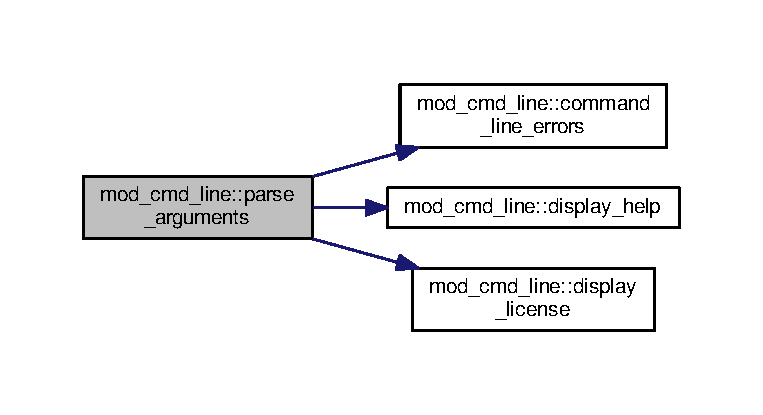
\includegraphics[width=350pt]{namespacemod__cmd__line_af3e6d85ae8e1f68f4c7c22e40bd3f3bb_cgraph}
\end{center}
\end{figure}




\subsection{Variable Documentation}
\index{mod\+\_\+cmd\+\_\+line@{mod\+\_\+cmd\+\_\+line}!arg@{arg}}
\index{arg@{arg}!mod\+\_\+cmd\+\_\+line@{mod\+\_\+cmd\+\_\+line}}
\subsubsection[{\texorpdfstring{arg}{arg}}]{\setlength{\rightskip}{0pt plus 5cm}character( len = 20 ), dimension(\+:), allocatable mod\+\_\+cmd\+\_\+line\+::arg}\hypertarget{namespacemod__cmd__line_a39002195e12526c3d97ff7ee81f9c00c}{}\label{namespacemod__cmd__line_a39002195e12526c3d97ff7ee81f9c00c}


Definition at line 24 of file mod\+\_\+cmd\+\_\+line.\+f90.



Referenced by command\+\_\+line\+\_\+errors(), display\+\_\+help(), display\+\_\+license(), and parse\+\_\+arguments().

\index{mod\+\_\+cmd\+\_\+line@{mod\+\_\+cmd\+\_\+line}!grid\+\_\+transl@{grid\+\_\+transl}}
\index{grid\+\_\+transl@{grid\+\_\+transl}!mod\+\_\+cmd\+\_\+line@{mod\+\_\+cmd\+\_\+line}}
\subsubsection[{\texorpdfstring{grid\+\_\+transl}{grid_transl}}]{\setlength{\rightskip}{0pt plus 5cm}character( len = 40 ) mod\+\_\+cmd\+\_\+line\+::grid\+\_\+transl = char(0)}\hypertarget{namespacemod__cmd__line_aa1ebd20914c6804b19cef6f2f1f5b8b9}{}\label{namespacemod__cmd__line_aa1ebd20914c6804b19cef6f2f1f5b8b9}


Definition at line 23 of file mod\+\_\+cmd\+\_\+line.\+f90.



Referenced by parse\+\_\+arguments(), and mod\+\_\+read\+\_\+grids\+::read\+\_\+translation\+\_\+grid().

\index{mod\+\_\+cmd\+\_\+line@{mod\+\_\+cmd\+\_\+line}!grid\+\_\+type@{grid\+\_\+type}}
\index{grid\+\_\+type@{grid\+\_\+type}!mod\+\_\+cmd\+\_\+line@{mod\+\_\+cmd\+\_\+line}}
\subsubsection[{\texorpdfstring{grid\+\_\+type}{grid_type}}]{\setlength{\rightskip}{0pt plus 5cm}character( len = 10 ) mod\+\_\+cmd\+\_\+line\+::grid\+\_\+type = char(0)}\hypertarget{namespacemod__cmd__line_ad92694e0caab203d3bc911dabb059271}{}\label{namespacemod__cmd__line_ad92694e0caab203d3bc911dabb059271}


Definition at line 22 of file mod\+\_\+cmd\+\_\+line.\+f90.



Referenced by mod\+\_\+resume\+::ending(), parse\+\_\+arguments(), and themis().

\index{mod\+\_\+cmd\+\_\+line@{mod\+\_\+cmd\+\_\+line}!irun@{irun}}
\index{irun@{irun}!mod\+\_\+cmd\+\_\+line@{mod\+\_\+cmd\+\_\+line}}
\subsubsection[{\texorpdfstring{irun}{irun}}]{\setlength{\rightskip}{0pt plus 5cm}character( len = 10 ) mod\+\_\+cmd\+\_\+line\+::irun = char(0)}\hypertarget{namespacemod__cmd__line_aae2bce3e1e50220133e7bd310a051881}{}\label{namespacemod__cmd__line_aae2bce3e1e50220133e7bd310a051881}


Definition at line 20 of file mod\+\_\+cmd\+\_\+line.\+f90.



Referenced by mod\+\_\+deallocate\+\_\+all\+::deallocate\+\_\+arrays(), mod\+\_\+resume\+::ending(), parse\+\_\+arguments(), and themis().

\index{mod\+\_\+cmd\+\_\+line@{mod\+\_\+cmd\+\_\+line}!rad@{rad}}
\index{rad@{rad}!mod\+\_\+cmd\+\_\+line@{mod\+\_\+cmd\+\_\+line}}
\subsubsection[{\texorpdfstring{rad}{rad}}]{\setlength{\rightskip}{0pt plus 5cm}real( kind = dp ) mod\+\_\+cmd\+\_\+line\+::rad = 0.\+0\+\_\+dp}\hypertarget{namespacemod__cmd__line_a726e623fa552ec6109d7f0e78545afe9}{}\label{namespacemod__cmd__line_a726e623fa552ec6109d7f0e78545afe9}


Definition at line 19 of file mod\+\_\+cmd\+\_\+line.\+f90.



Referenced by mod\+\_\+read\+\_\+grids\+::build\+\_\+translation\+\_\+sphere(), mod\+\_\+resume\+::ending(), and parse\+\_\+arguments().

\index{mod\+\_\+cmd\+\_\+line@{mod\+\_\+cmd\+\_\+line}!str\+\_\+rad@{str\+\_\+rad}}
\index{str\+\_\+rad@{str\+\_\+rad}!mod\+\_\+cmd\+\_\+line@{mod\+\_\+cmd\+\_\+line}}
\subsubsection[{\texorpdfstring{str\+\_\+rad}{str_rad}}]{\setlength{\rightskip}{0pt plus 5cm}character( len = 10 ) mod\+\_\+cmd\+\_\+line\+::str\+\_\+rad = char(0)}\hypertarget{namespacemod__cmd__line_aa7def1b6cf5f62c8473902ef9fc7f307}{}\label{namespacemod__cmd__line_aa7def1b6cf5f62c8473902ef9fc7f307}


Definition at line 21 of file mod\+\_\+cmd\+\_\+line.\+f90.


\hypertarget{namespacemod__constants}{}\section{mod\+\_\+constants Module Reference}
\label{namespacemod__constants}\index{mod\+\_\+constants@{mod\+\_\+constants}}


This module defines a set constants.  


\subsection*{Variables}
\begin{DoxyCompactItemize}
\item 
integer, parameter, public \hyperlink{namespacemod__constants_ac7aeda7f1802c4ef2a4780773c028214}{dp} = selected\+\_\+real\+\_\+kind(15, 307)
\item 
integer, parameter, public \hyperlink{namespacemod__constants_af0d7aefb6fb852492ee0db77744a412d}{sp} = selected\+\_\+real\+\_\+kind(6, 37)
\item 
real(kind=\hyperlink{namespacemod__constants_ac7aeda7f1802c4ef2a4780773c028214}{dp}), parameter, public \hyperlink{namespacemod__constants_a04c6845722711f5522458ed34969cdc3}{pi} = 3.\+14159265358979\+\_\+\+DP
\item 
real(kind=\hyperlink{namespacemod__constants_ac7aeda7f1802c4ef2a4780773c028214}{dp}), parameter, public \hyperlink{namespacemod__constants_a505a7c2ab1e1b2fa75db18a1d3e133b4}{deg2rad} = 180.\+0\+\_\+\+D\+P / PI
\item 
real(kind=\hyperlink{namespacemod__constants_ac7aeda7f1802c4ef2a4780773c028214}{dp}), parameter, public \hyperlink{namespacemod__constants_af84a9ff68ff16d57560ea196b8e560d4}{kb} = 0.\+0083144621\+\_\+\+DP
\item 
real(kind=\hyperlink{namespacemod__constants_ac7aeda7f1802c4ef2a4780773c028214}{dp}), parameter, public \hyperlink{namespacemod__constants_a0943b8c8fb52658fb3d4370e5defb34b}{ccon} = 1389.\+354578\+\_\+\+DP
\item 
real(kind=\hyperlink{namespacemod__constants_ac7aeda7f1802c4ef2a4780773c028214}{dp}), parameter, public \hyperlink{namespacemod__constants_a1f06c759fc8a61d66f343865300c37d1}{fpzero} = tiny(1.\+0\+\_\+\+D\+P)
\item 
real(kind=\hyperlink{namespacemod__constants_ac7aeda7f1802c4ef2a4780773c028214}{dp}), parameter, public \hyperlink{namespacemod__constants_a64820d61363b4adcee8f4f810662e836}{fpinf} = huge(1.\+0\+\_\+\+D\+P)
\item 
real(kind=\hyperlink{namespacemod__constants_ac7aeda7f1802c4ef2a4780773c028214}{dp}), parameter, public \hyperlink{namespacemod__constants_ab31d074fb8a49a9991d7d6e3d4904d59}{ms} = 0.\+001\+\_\+\+DP
\item 
character(len=11), parameter \hyperlink{namespacemod__constants_a41cb897f7d31e58ab3c2b2f7ecf86983}{int\+\_\+alphabet} = \textquotesingle{}1234567890\textquotesingle{}
\item 
character(len=12), parameter \hyperlink{namespacemod__constants_a4b168363a34adf3e1236769aa1ec0fed}{float\+\_\+alphabet} = \textquotesingle{}.-\/1234567890\textquotesingle{}
\item 
character(len=66), parameter \hyperlink{namespacemod__constants_a1d9e53f57f87f727d4dd13f1dd4b8e45}{char\+\_\+alphabet} = \textquotesingle{}abcdefghijklmnopqrstuvwxyz\+A\+B\+C\+D\+E\+F\+G\+H\+I\+J\+K\+L\+M\+N\+O\+P\+Q\+R\+S\+T\+U\+V\+W\+X\+Y\+Z.\+\_\+-\/1234567890 \textquotesingle{}
\item 
character(len=74), parameter \hyperlink{namespacemod__constants_ab55dac3c52ff6b1034697c6e83ac76d8}{dashline} = repeat(\textquotesingle{}-\/\textquotesingle{}, 74)
\end{DoxyCompactItemize}


\subsection{Detailed Description}
This module defines a set constants. 

\begin{DoxyAuthor}{Author}
Felippe M. Colombari
\begin{DoxyItemize}
\item Laboratório de Química Teórica, L\+QT -- U\+F\+S\+Car 
\end{DoxyItemize}
\end{DoxyAuthor}
\begin{DoxyDate}{Date}
-\/ Dec, 2017
\begin{DoxyItemize}
\item module created 
\end{DoxyItemize}
\end{DoxyDate}


\subsection{Variable Documentation}
\index{mod\+\_\+constants@{mod\+\_\+constants}!ccon@{ccon}}
\index{ccon@{ccon}!mod\+\_\+constants@{mod\+\_\+constants}}
\subsubsection[{\texorpdfstring{ccon}{ccon}}]{\setlength{\rightskip}{0pt plus 5cm}real( kind = {\bf dp} ), parameter, public mod\+\_\+constants\+::ccon = 1389.\+354578\+\_\+\+DP}\hypertarget{namespacemod__constants_a0943b8c8fb52658fb3d4370e5defb34b}{}\label{namespacemod__constants_a0943b8c8fb52658fb3d4370e5defb34b}


Definition at line 24 of file mod\+\_\+constants.\+f90.



Referenced by mod\+\_\+pot\+\_\+ljc\+::calc\+\_\+ljc\+\_\+energy().

\index{mod\+\_\+constants@{mod\+\_\+constants}!char\+\_\+alphabet@{char\+\_\+alphabet}}
\index{char\+\_\+alphabet@{char\+\_\+alphabet}!mod\+\_\+constants@{mod\+\_\+constants}}
\subsubsection[{\texorpdfstring{char\+\_\+alphabet}{char_alphabet}}]{\setlength{\rightskip}{0pt plus 5cm}character( len = 66 ), parameter mod\+\_\+constants\+::char\+\_\+alphabet = \textquotesingle{}abcdefghijklmnopqrstuvwxyz\+A\+B\+C\+D\+E\+F\+G\+H\+I\+J\+K\+L\+M\+N\+O\+P\+Q\+R\+S\+T\+U\+V\+W\+X\+Y\+Z.\+\_\+-\/1234567890 \textquotesingle{}}\hypertarget{namespacemod__constants_a1d9e53f57f87f727d4dd13f1dd4b8e45}{}\label{namespacemod__constants_a1d9e53f57f87f727d4dd13f1dd4b8e45}


Definition at line 31 of file mod\+\_\+constants.\+f90.



Referenced by mod\+\_\+cmd\+\_\+line\+::parse\+\_\+arguments().

\index{mod\+\_\+constants@{mod\+\_\+constants}!dashline@{dashline}}
\index{dashline@{dashline}!mod\+\_\+constants@{mod\+\_\+constants}}
\subsubsection[{\texorpdfstring{dashline}{dashline}}]{\setlength{\rightskip}{0pt plus 5cm}character( len = 74 ), parameter mod\+\_\+constants\+::dashline = repeat(\textquotesingle{}-\/\textquotesingle{}, 74)}\hypertarget{namespacemod__constants_ab55dac3c52ff6b1034697c6e83ac76d8}{}\label{namespacemod__constants_ab55dac3c52ff6b1034697c6e83ac76d8}


Definition at line 33 of file mod\+\_\+constants.\+f90.



Referenced by mod\+\_\+pot\+\_\+ljc\+::check\+\_\+ljc\+\_\+params(), mod\+\_\+read\+\_\+grids\+::check\+\_\+moves(), mod\+\_\+cmd\+\_\+line\+::command\+\_\+line\+\_\+errors(), mod\+\_\+cmd\+\_\+line\+::display\+\_\+help(), mod\+\_\+cmd\+\_\+line\+::display\+\_\+license(), mod\+\_\+resume\+::ending(), mod\+\_\+input\+\_\+read\+::input\+\_\+errors(), mod\+\_\+cmd\+\_\+line\+::parse\+\_\+arguments(), and mod\+\_\+resume\+::sort\+\_\+output().

\index{mod\+\_\+constants@{mod\+\_\+constants}!deg2rad@{deg2rad}}
\index{deg2rad@{deg2rad}!mod\+\_\+constants@{mod\+\_\+constants}}
\subsubsection[{\texorpdfstring{deg2rad}{deg2rad}}]{\setlength{\rightskip}{0pt plus 5cm}real( kind = {\bf dp} ), parameter, public mod\+\_\+constants\+::deg2rad = 180.\+0\+\_\+\+D\+P / PI}\hypertarget{namespacemod__constants_a505a7c2ab1e1b2fa75db18a1d3e133b4}{}\label{namespacemod__constants_a505a7c2ab1e1b2fa75db18a1d3e133b4}


Definition at line 22 of file mod\+\_\+constants.\+f90.



Referenced by mod\+\_\+read\+\_\+xyz\+::rotate\+\_\+xyz().

\index{mod\+\_\+constants@{mod\+\_\+constants}!dp@{dp}}
\index{dp@{dp}!mod\+\_\+constants@{mod\+\_\+constants}}
\subsubsection[{\texorpdfstring{dp}{dp}}]{\setlength{\rightskip}{0pt plus 5cm}integer, parameter, public mod\+\_\+constants\+::dp = selected\+\_\+real\+\_\+kind(15, 307)}\hypertarget{namespacemod__constants_ac7aeda7f1802c4ef2a4780773c028214}{}\label{namespacemod__constants_ac7aeda7f1802c4ef2a4780773c028214}


Definition at line 18 of file mod\+\_\+constants.\+f90.



Referenced by mod\+\_\+vmd\+::write\+\_\+vmd\+\_\+files().

\index{mod\+\_\+constants@{mod\+\_\+constants}!float\+\_\+alphabet@{float\+\_\+alphabet}}
\index{float\+\_\+alphabet@{float\+\_\+alphabet}!mod\+\_\+constants@{mod\+\_\+constants}}
\subsubsection[{\texorpdfstring{float\+\_\+alphabet}{float_alphabet}}]{\setlength{\rightskip}{0pt plus 5cm}character( len = 12 ), parameter mod\+\_\+constants\+::float\+\_\+alphabet = \textquotesingle{}.-\/1234567890\textquotesingle{}}\hypertarget{namespacemod__constants_a4b168363a34adf3e1236769aa1ec0fed}{}\label{namespacemod__constants_a4b168363a34adf3e1236769aa1ec0fed}


Definition at line 30 of file mod\+\_\+constants.\+f90.



Referenced by mod\+\_\+cmd\+\_\+line\+::parse\+\_\+arguments(), and mod\+\_\+input\+\_\+read\+::read\+\_\+input().

\index{mod\+\_\+constants@{mod\+\_\+constants}!fpinf@{fpinf}}
\index{fpinf@{fpinf}!mod\+\_\+constants@{mod\+\_\+constants}}
\subsubsection[{\texorpdfstring{fpinf}{fpinf}}]{\setlength{\rightskip}{0pt plus 5cm}real( kind = {\bf dp} ), parameter, public mod\+\_\+constants\+::fpinf = huge(1.\+0\+\_\+\+D\+P)}\hypertarget{namespacemod__constants_a64820d61363b4adcee8f4f810662e836}{}\label{namespacemod__constants_a64820d61363b4adcee8f4f810662e836}


Definition at line 26 of file mod\+\_\+constants.\+f90.



Referenced by mod\+\_\+search\+::sort\+\_\+energy(), and mod\+\_\+resume\+::sort\+\_\+output().

\index{mod\+\_\+constants@{mod\+\_\+constants}!fpzero@{fpzero}}
\index{fpzero@{fpzero}!mod\+\_\+constants@{mod\+\_\+constants}}
\subsubsection[{\texorpdfstring{fpzero}{fpzero}}]{\setlength{\rightskip}{0pt plus 5cm}real( kind = {\bf dp} ), parameter, public mod\+\_\+constants\+::fpzero = tiny(1.\+0\+\_\+\+D\+P)}\hypertarget{namespacemod__constants_a1f06c759fc8a61d66f343865300c37d1}{}\label{namespacemod__constants_a1f06c759fc8a61d66f343865300c37d1}


Definition at line 25 of file mod\+\_\+constants.\+f90.

\index{mod\+\_\+constants@{mod\+\_\+constants}!int\+\_\+alphabet@{int\+\_\+alphabet}}
\index{int\+\_\+alphabet@{int\+\_\+alphabet}!mod\+\_\+constants@{mod\+\_\+constants}}
\subsubsection[{\texorpdfstring{int\+\_\+alphabet}{int_alphabet}}]{\setlength{\rightskip}{0pt plus 5cm}character( len = 11 ), parameter mod\+\_\+constants\+::int\+\_\+alphabet = \textquotesingle{}1234567890\textquotesingle{}}\hypertarget{namespacemod__constants_a41cb897f7d31e58ab3c2b2f7ecf86983}{}\label{namespacemod__constants_a41cb897f7d31e58ab3c2b2f7ecf86983}


Definition at line 29 of file mod\+\_\+constants.\+f90.



Referenced by mod\+\_\+input\+\_\+read\+::read\+\_\+input().

\index{mod\+\_\+constants@{mod\+\_\+constants}!kb@{kb}}
\index{kb@{kb}!mod\+\_\+constants@{mod\+\_\+constants}}
\subsubsection[{\texorpdfstring{kb}{kb}}]{\setlength{\rightskip}{0pt plus 5cm}real( kind = {\bf dp} ), parameter, public mod\+\_\+constants\+::kb = 0.\+0083144621\+\_\+\+DP}\hypertarget{namespacemod__constants_af84a9ff68ff16d57560ea196b8e560d4}{}\label{namespacemod__constants_af84a9ff68ff16d57560ea196b8e560d4}


Definition at line 23 of file mod\+\_\+constants.\+f90.



Referenced by mod\+\_\+loops\+::calc(), mod\+\_\+loops\+::calc\+\_\+ztotal(), and mod\+\_\+loops\+::recalc().

\index{mod\+\_\+constants@{mod\+\_\+constants}!ms@{ms}}
\index{ms@{ms}!mod\+\_\+constants@{mod\+\_\+constants}}
\subsubsection[{\texorpdfstring{ms}{ms}}]{\setlength{\rightskip}{0pt plus 5cm}real( kind = {\bf dp} ), parameter, public mod\+\_\+constants\+::ms = 0.\+001\+\_\+\+DP}\hypertarget{namespacemod__constants_ab31d074fb8a49a9991d7d6e3d4904d59}{}\label{namespacemod__constants_ab31d074fb8a49a9991d7d6e3d4904d59}


Definition at line 27 of file mod\+\_\+constants.\+f90.

\index{mod\+\_\+constants@{mod\+\_\+constants}!pi@{pi}}
\index{pi@{pi}!mod\+\_\+constants@{mod\+\_\+constants}}
\subsubsection[{\texorpdfstring{pi}{pi}}]{\setlength{\rightskip}{0pt plus 5cm}real( kind = {\bf dp} ), parameter, public mod\+\_\+constants\+::pi = 3.\+14159265358979\+\_\+\+DP}\hypertarget{namespacemod__constants_a04c6845722711f5522458ed34969cdc3}{}\label{namespacemod__constants_a04c6845722711f5522458ed34969cdc3}


Definition at line 21 of file mod\+\_\+constants.\+f90.



Referenced by mod\+\_\+read\+\_\+xyz\+::align\+\_\+xyz().

\index{mod\+\_\+constants@{mod\+\_\+constants}!sp@{sp}}
\index{sp@{sp}!mod\+\_\+constants@{mod\+\_\+constants}}
\subsubsection[{\texorpdfstring{sp}{sp}}]{\setlength{\rightskip}{0pt plus 5cm}integer, parameter, public mod\+\_\+constants\+::sp = selected\+\_\+real\+\_\+kind(6, 37)}\hypertarget{namespacemod__constants_af0d7aefb6fb852492ee0db77744a412d}{}\label{namespacemod__constants_af0d7aefb6fb852492ee0db77744a412d}


Definition at line 19 of file mod\+\_\+constants.\+f90.


\hypertarget{namespacemod__deallocate__all}{}\section{mod\+\_\+deallocate\+\_\+all Module Reference}
\label{namespacemod__deallocate__all}\index{mod\+\_\+deallocate\+\_\+all@{mod\+\_\+deallocate\+\_\+all}}


This module constains instructions to deallocate all arrays prior to program termination.  


\subsection*{Functions/\+Subroutines}
\begin{DoxyCompactItemize}
\item 
subroutine, public \hyperlink{namespacemod__deallocate__all_a03994854d5404353882da36b59ca3098}{deallocate\+\_\+arrays}
\end{DoxyCompactItemize}


\subsection{Detailed Description}
This module constains instructions to deallocate all arrays prior to program termination. 

\begin{DoxyAuthor}{Author}
Felippe M. Colombari
\begin{DoxyItemize}
\item Laboratório de Química Teórica, L\+QT -- U\+F\+S\+Car 
\end{DoxyItemize}
\end{DoxyAuthor}
\begin{DoxyDate}{Date}
-\/ Dec, 2017
\begin{DoxyItemize}
\item independent module created 
\end{DoxyItemize}
\end{DoxyDate}
\begin{DoxyNote}{Note}

\begin{DoxyItemize}
\item to check for memory leaks and/or final status of allocatable arrays please use\+: ~\newline
 valgrind --leak-\/check=full --show-\/leak-\/kinds=all -\/v ./themis \mbox{[} options \mbox{]}
\item to check memory usage along execution, please use\+: ~\newline
 valgrind --tool=massif ./themis \mbox{[}options\mbox{]} 
\end{DoxyItemize}
\end{DoxyNote}


\subsection{Function/\+Subroutine Documentation}
\mbox{\Hypertarget{namespacemod__deallocate__all_a03994854d5404353882da36b59ca3098}\label{namespacemod__deallocate__all_a03994854d5404353882da36b59ca3098}} 
\index{mod\+\_\+deallocate\+\_\+all@{mod\+\_\+deallocate\+\_\+all}!deallocate\+\_\+arrays@{deallocate\+\_\+arrays}}
\index{deallocate\+\_\+arrays@{deallocate\+\_\+arrays}!mod\+\_\+deallocate\+\_\+all@{mod\+\_\+deallocate\+\_\+all}}
\subsubsection{\texorpdfstring{deallocate\+\_\+arrays()}{deallocate\_arrays()}}
{\footnotesize\ttfamily subroutine, public mod\+\_\+deallocate\+\_\+all\+::deallocate\+\_\+arrays (\begin{DoxyParamCaption}{ }\end{DoxyParamCaption})}



Definition at line 31 of file mod\+\_\+deallocate\+\_\+all.\+f90.



References mod\+\_\+input\+\_\+read\+::atom\+\_\+overlap, mod\+\_\+read\+\_\+grids\+::grid\+\_\+reo, mod\+\_\+read\+\_\+grids\+::grid\+\_\+trans, mod\+\_\+input\+\_\+read\+::inter\+\_\+energy, mod\+\_\+cmd\+\_\+line\+::irun, mod\+\_\+loops\+::min\+\_\+ener\+\_\+t, mod\+\_\+read\+\_\+molecules\+::mol1, mod\+\_\+pot\+\_\+bhc\+::mol1\+\_\+bhc, mod\+\_\+read\+\_\+molecules\+::mol2, mod\+\_\+pot\+\_\+bhc\+::mol2\+\_\+bhc, mod\+\_\+pot\+\_\+ljc\+::mol2\+\_\+ljc, mod\+\_\+read\+\_\+grids\+::phir, mod\+\_\+input\+\_\+read\+::potential, mod\+\_\+read\+\_\+grids\+::probt, mod\+\_\+read\+\_\+grids\+::rr, mod\+\_\+read\+\_\+grids\+::sumvexpvrot, mod\+\_\+read\+\_\+grids\+::thetar, and mod\+\_\+read\+\_\+grids\+::zrot.



Referenced by themis().


\hypertarget{namespacemod__input__read}{}\section{mod\+\_\+input\+\_\+read Module Reference}
\label{namespacemod__input__read}\index{mod\+\_\+input\+\_\+read@{mod\+\_\+input\+\_\+read}}


This module contains a routine for I\+N\+P\+UT reading and checking.  


\subsection*{Functions/\+Subroutines}
\begin{DoxyCompactItemize}
\item 
subroutine, public \hyperlink{namespacemod__input__read_ae27abd188ee109221a29ed77b68fb6d9}{read\+\_\+input\+\_\+file}
\item 
subroutine \hyperlink{namespacemod__input__read_a396026faa10ab3698196930dfb90690b}{check\+\_\+keys}
\end{DoxyCompactItemize}
\subsection*{Variables}
\begin{DoxyCompactItemize}
\item 
character(len=10), public \hyperlink{namespacemod__input__read_aaf9a85c22da4f3ae7bbcc9ba72d783dd}{potential} = char(0)
\item 
character(len=10), public \hyperlink{namespacemod__input__read_a02f99bb5470feaf35ab2fc228c797f64}{writeframe} = char(0)
\item 
character(len=5), public \hyperlink{namespacemod__input__read_af757b04e60563ace187ed465be839553}{wrtxtc} = char(0)
\item 
real(kind=dp), public \hyperlink{namespacemod__input__read_a584082766fe740d0c5f3975d3d44426b}{temp} = 0.\+0
\item 
real(kind=dp), public \hyperlink{namespacemod__input__read_ad2ddb7a8a7af94da8a7d12c6e3ab9899}{rcut\+\_\+sqr} = 0.\+0
\item 
real(kind=dp), public \hyperlink{namespacemod__input__read_a9ef9305fdc4e5164af51f0da464c36c0}{cutoff\+\_\+sqr} = 0.\+0
\item 
real(kind=dp), public \hyperlink{namespacemod__input__read_a3f3cf0bf8b5ebc1886d493eda84eecf4}{max\+\_\+gyr} = 0.\+0
\item 
integer, public \hyperlink{namespacemod__input__read_a55be21acb2dc4800c8d3cecf28e4166f}{scale\+\_\+factor} = 0
\item 
integer, public \hyperlink{namespacemod__input__read_ae958873dff0867f0aa04dbf6cd8a1166}{trans\+\_\+factor} = 0
\item 
integer, public \hyperlink{namespacemod__input__read_ab81a502be00c6796c9474d728db96041}{reo\+\_\+factor} = 0
\item 
integer, public \hyperlink{namespacemod__input__read_a76985d277087bc52f1b81814fe4c50bc}{gyr\+\_\+factor} = 0
\item 
integer, public \hyperlink{namespacemod__input__read_ae009fc7ba8243327aec0bed57f18b515}{ref1} = 0
\item 
integer, public \hyperlink{namespacemod__input__read_a72ae0812ca16c5cbb7eb3cbe12bafb58}{ref2} = 0
\item 
integer, public \hyperlink{namespacemod__input__read_a6e68357b53efca593488929b4554838d}{vector1} = 0
\item 
integer, public \hyperlink{namespacemod__input__read_a4f1ca96e94c5298b480fa8d43bb1b915}{vector2} = 0
\item 
integer, public \hyperlink{namespacemod__input__read_a8aa83854894f2e947a4e1015697433d0}{nstruc} = 0
\item 
logical, dimension(\+:,\+:,\+:), allocatable, public \hyperlink{namespacemod__input__read_ada662a2d234d567ce7da80355d2c9e21}{atom\+\_\+overlap}
\item 
real(kind=dp), dimension(\+:,\+:,\+:), allocatable, public \hyperlink{namespacemod__input__read_a59e3573d7d32b72bd699ac1708e70908}{inter\+\_\+energy}
\end{DoxyCompactItemize}


\subsection{Detailed Description}
This module contains a routine for I\+N\+P\+UT reading and checking. 

\begin{DoxyAuthor}{Author}
Felippe M. Colombari
\begin{DoxyItemize}
\item Laboratório de Química Teórica, L\+QT -- U\+F\+S\+Car 
\end{DoxyItemize}
\end{DoxyAuthor}
\begin{DoxyDate}{Date}
-\/ Jun, 2017
\begin{DoxyItemize}
\item independent module created 
\end{DoxyItemize}

-\/ Jan, 2018
\begin{DoxyItemize}
\item support added 
\end{DoxyItemize}
\end{DoxyDate}
\begin{DoxyNote}{Note}
update error condition by error\+\_\+handling module added by Asdrubal Lozada-\/\+Blanco 
\end{DoxyNote}
\begin{DoxyDate}{Date}
-\/ Nov 2019 
\end{DoxyDate}


\subsection{Function/\+Subroutine Documentation}
\mbox{\Hypertarget{namespacemod__input__read_a396026faa10ab3698196930dfb90690b}\label{namespacemod__input__read_a396026faa10ab3698196930dfb90690b}} 
\index{mod\+\_\+input\+\_\+read@{mod\+\_\+input\+\_\+read}!check\+\_\+keys@{check\+\_\+keys}}
\index{check\+\_\+keys@{check\+\_\+keys}!mod\+\_\+input\+\_\+read@{mod\+\_\+input\+\_\+read}}
\subsubsection{\texorpdfstring{check\+\_\+keys()}{check\_keys()}}
{\footnotesize\ttfamily subroutine mod\+\_\+input\+\_\+read\+::check\+\_\+keys (\begin{DoxyParamCaption}{ }\end{DoxyParamCaption})}



Definition at line 619 of file mod\+\_\+input\+\_\+read.\+f90.



References mod\+\_\+cmd\+\_\+line\+::grid\+\_\+type, and writeframe.



Referenced by read\+\_\+input\+\_\+file().

\mbox{\Hypertarget{namespacemod__input__read_ae27abd188ee109221a29ed77b68fb6d9}\label{namespacemod__input__read_ae27abd188ee109221a29ed77b68fb6d9}} 
\index{mod\+\_\+input\+\_\+read@{mod\+\_\+input\+\_\+read}!read\+\_\+input\+\_\+file@{read\+\_\+input\+\_\+file}}
\index{read\+\_\+input\+\_\+file@{read\+\_\+input\+\_\+file}!mod\+\_\+input\+\_\+read@{mod\+\_\+input\+\_\+read}}
\subsubsection{\texorpdfstring{read\+\_\+input\+\_\+file()}{read\_input\_file()}}
{\footnotesize\ttfamily subroutine, public mod\+\_\+input\+\_\+read\+::read\+\_\+input\+\_\+file (\begin{DoxyParamCaption}{ }\end{DoxyParamCaption})}



Definition at line 78 of file mod\+\_\+input\+\_\+read.\+f90.



References check\+\_\+keys(), cutoff\+\_\+sqr, mod\+\_\+constants\+::float\+\_\+alphabet, mod\+\_\+constants\+::fpinf, gyr\+\_\+factor, mod\+\_\+inquire\+::inquire\+\_\+file(), mod\+\_\+constants\+::int\+\_\+alphabet, max\+\_\+gyr, nstruc, potential, rcut\+\_\+sqr, ref1, ref2, reo\+\_\+factor, scale\+\_\+factor, temp, trans\+\_\+factor, vector1, vector2, writeframe, and wrtxtc.



Referenced by themis().

Here is the call graph for this function\+:
\nopagebreak
\begin{figure}[H]
\begin{center}
\leavevmode
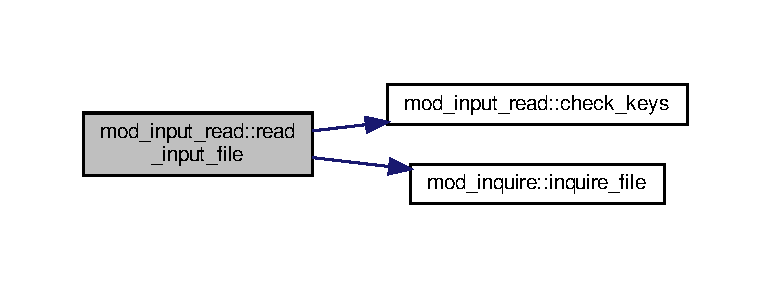
\includegraphics[width=350pt]{namespacemod__input__read_ae27abd188ee109221a29ed77b68fb6d9_cgraph}
\end{center}
\end{figure}


\subsection{Variable Documentation}
\mbox{\Hypertarget{namespacemod__input__read_ada662a2d234d567ce7da80355d2c9e21}\label{namespacemod__input__read_ada662a2d234d567ce7da80355d2c9e21}} 
\index{mod\+\_\+input\+\_\+read@{mod\+\_\+input\+\_\+read}!atom\+\_\+overlap@{atom\+\_\+overlap}}
\index{atom\+\_\+overlap@{atom\+\_\+overlap}!mod\+\_\+input\+\_\+read@{mod\+\_\+input\+\_\+read}}
\subsubsection{\texorpdfstring{atom\+\_\+overlap}{atom\_overlap}}
{\footnotesize\ttfamily logical, dimension(\+:,\+:,\+:), allocatable, public mod\+\_\+input\+\_\+read\+::atom\+\_\+overlap}



Definition at line 70 of file mod\+\_\+input\+\_\+read.\+f90.



Referenced by mod\+\_\+loops\+::calc(), mod\+\_\+pot\+\_\+bhc\+::calc\+\_\+bhc\+\_\+energy(), mod\+\_\+pot\+\_\+ljc\+::calc\+\_\+ljc\+\_\+energy(), mod\+\_\+pot\+\_\+ljc\+\_\+pair\+::calc\+\_\+ljc\+\_\+pair\+\_\+energy(), mod\+\_\+read\+\_\+molecules\+::calc\+\_\+none\+\_\+energy(), mod\+\_\+deallocate\+\_\+all\+::deallocate\+\_\+arrays(), and mod\+\_\+resume\+::ending().

\mbox{\Hypertarget{namespacemod__input__read_a9ef9305fdc4e5164af51f0da464c36c0}\label{namespacemod__input__read_a9ef9305fdc4e5164af51f0da464c36c0}} 
\index{mod\+\_\+input\+\_\+read@{mod\+\_\+input\+\_\+read}!cutoff\+\_\+sqr@{cutoff\+\_\+sqr}}
\index{cutoff\+\_\+sqr@{cutoff\+\_\+sqr}!mod\+\_\+input\+\_\+read@{mod\+\_\+input\+\_\+read}}
\subsubsection{\texorpdfstring{cutoff\+\_\+sqr}{cutoff\_sqr}}
{\footnotesize\ttfamily real( kind = dp ), public mod\+\_\+input\+\_\+read\+::cutoff\+\_\+sqr = 0.\+0}



Definition at line 40 of file mod\+\_\+input\+\_\+read.\+f90.



Referenced by mod\+\_\+pot\+\_\+ljc\+\_\+pair\+::calc\+\_\+ljc\+\_\+pair\+\_\+energy(), and read\+\_\+input\+\_\+file().

\mbox{\Hypertarget{namespacemod__input__read_a76985d277087bc52f1b81814fe4c50bc}\label{namespacemod__input__read_a76985d277087bc52f1b81814fe4c50bc}} 
\index{mod\+\_\+input\+\_\+read@{mod\+\_\+input\+\_\+read}!gyr\+\_\+factor@{gyr\+\_\+factor}}
\index{gyr\+\_\+factor@{gyr\+\_\+factor}!mod\+\_\+input\+\_\+read@{mod\+\_\+input\+\_\+read}}
\subsubsection{\texorpdfstring{gyr\+\_\+factor}{gyr\_factor}}
{\footnotesize\ttfamily integer, public mod\+\_\+input\+\_\+read\+::gyr\+\_\+factor = 0}



Definition at line 45 of file mod\+\_\+input\+\_\+read.\+f90.



Referenced by mod\+\_\+loops\+::calc(), mod\+\_\+loops\+::calc\+\_\+ztotal(), mod\+\_\+read\+\_\+grids\+::check\+\_\+moves(), mod\+\_\+search\+::count\+\_\+structures(), read\+\_\+input\+\_\+file(), mod\+\_\+loops\+::recalc(), and mod\+\_\+read\+\_\+molecules\+::rotate\+\_\+molecule().

\mbox{\Hypertarget{namespacemod__input__read_a59e3573d7d32b72bd699ac1708e70908}\label{namespacemod__input__read_a59e3573d7d32b72bd699ac1708e70908}} 
\index{mod\+\_\+input\+\_\+read@{mod\+\_\+input\+\_\+read}!inter\+\_\+energy@{inter\+\_\+energy}}
\index{inter\+\_\+energy@{inter\+\_\+energy}!mod\+\_\+input\+\_\+read@{mod\+\_\+input\+\_\+read}}
\subsubsection{\texorpdfstring{inter\+\_\+energy}{inter\_energy}}
{\footnotesize\ttfamily real( kind = dp ), dimension(\+:,\+:,\+:), allocatable, public mod\+\_\+input\+\_\+read\+::inter\+\_\+energy}



Definition at line 71 of file mod\+\_\+input\+\_\+read.\+f90.



Referenced by mod\+\_\+loops\+::calc(), mod\+\_\+pot\+\_\+bhc\+::calc\+\_\+bhc\+\_\+energy(), mod\+\_\+pot\+\_\+ljc\+::calc\+\_\+ljc\+\_\+energy(), mod\+\_\+pot\+\_\+ljc\+\_\+pair\+::calc\+\_\+ljc\+\_\+pair\+\_\+energy(), mod\+\_\+read\+\_\+molecules\+::calc\+\_\+none\+\_\+energy(), mod\+\_\+loops\+::calc\+\_\+ztotal(), mod\+\_\+search\+::count\+\_\+structures(), mod\+\_\+deallocate\+\_\+all\+::deallocate\+\_\+arrays(), mod\+\_\+loops\+::recalc(), and mod\+\_\+search\+::sort\+\_\+energy().

\mbox{\Hypertarget{namespacemod__input__read_a3f3cf0bf8b5ebc1886d493eda84eecf4}\label{namespacemod__input__read_a3f3cf0bf8b5ebc1886d493eda84eecf4}} 
\index{mod\+\_\+input\+\_\+read@{mod\+\_\+input\+\_\+read}!max\+\_\+gyr@{max\+\_\+gyr}}
\index{max\+\_\+gyr@{max\+\_\+gyr}!mod\+\_\+input\+\_\+read@{mod\+\_\+input\+\_\+read}}
\subsubsection{\texorpdfstring{max\+\_\+gyr}{max\_gyr}}
{\footnotesize\ttfamily real( kind = dp ), public mod\+\_\+input\+\_\+read\+::max\+\_\+gyr = 0.\+0}



Definition at line 41 of file mod\+\_\+input\+\_\+read.\+f90.



Referenced by mod\+\_\+read\+\_\+grids\+::check\+\_\+moves(), read\+\_\+input\+\_\+file(), and mod\+\_\+read\+\_\+molecules\+::rotate\+\_\+molecule().

\mbox{\Hypertarget{namespacemod__input__read_a8aa83854894f2e947a4e1015697433d0}\label{namespacemod__input__read_a8aa83854894f2e947a4e1015697433d0}} 
\index{mod\+\_\+input\+\_\+read@{mod\+\_\+input\+\_\+read}!nstruc@{nstruc}}
\index{nstruc@{nstruc}!mod\+\_\+input\+\_\+read@{mod\+\_\+input\+\_\+read}}
\subsubsection{\texorpdfstring{nstruc}{nstruc}}
{\footnotesize\ttfamily integer, public mod\+\_\+input\+\_\+read\+::nstruc = 0}



Definition at line 50 of file mod\+\_\+input\+\_\+read.\+f90.



Referenced by read\+\_\+input\+\_\+file(), mod\+\_\+search\+::search\+\_\+structures(), and mod\+\_\+search\+::sort\+\_\+energy().

\mbox{\Hypertarget{namespacemod__input__read_aaf9a85c22da4f3ae7bbcc9ba72d783dd}\label{namespacemod__input__read_aaf9a85c22da4f3ae7bbcc9ba72d783dd}} 
\index{mod\+\_\+input\+\_\+read@{mod\+\_\+input\+\_\+read}!potential@{potential}}
\index{potential@{potential}!mod\+\_\+input\+\_\+read@{mod\+\_\+input\+\_\+read}}
\subsubsection{\texorpdfstring{potential}{potential}}
{\footnotesize\ttfamily character( len = 10 ), public mod\+\_\+input\+\_\+read\+::potential = char(0)}



Definition at line 33 of file mod\+\_\+input\+\_\+read.\+f90.



Referenced by mod\+\_\+loops\+::calc(), mod\+\_\+deallocate\+\_\+all\+::deallocate\+\_\+arrays(), mod\+\_\+resume\+::ending(), read\+\_\+input\+\_\+file(), mod\+\_\+loops\+::recalc(), and themis().

\mbox{\Hypertarget{namespacemod__input__read_ad2ddb7a8a7af94da8a7d12c6e3ab9899}\label{namespacemod__input__read_ad2ddb7a8a7af94da8a7d12c6e3ab9899}} 
\index{mod\+\_\+input\+\_\+read@{mod\+\_\+input\+\_\+read}!rcut\+\_\+sqr@{rcut\+\_\+sqr}}
\index{rcut\+\_\+sqr@{rcut\+\_\+sqr}!mod\+\_\+input\+\_\+read@{mod\+\_\+input\+\_\+read}}
\subsubsection{\texorpdfstring{rcut\+\_\+sqr}{rcut\_sqr}}
{\footnotesize\ttfamily real( kind = dp ), public mod\+\_\+input\+\_\+read\+::rcut\+\_\+sqr = 0.\+0}



Definition at line 38 of file mod\+\_\+input\+\_\+read.\+f90.



Referenced by mod\+\_\+pot\+\_\+bhc\+::calc\+\_\+bhc\+\_\+energy(), mod\+\_\+pot\+\_\+ljc\+::calc\+\_\+ljc\+\_\+energy(), mod\+\_\+pot\+\_\+ljc\+\_\+pair\+::calc\+\_\+ljc\+\_\+pair\+\_\+energy(), and read\+\_\+input\+\_\+file().

\mbox{\Hypertarget{namespacemod__input__read_ae009fc7ba8243327aec0bed57f18b515}\label{namespacemod__input__read_ae009fc7ba8243327aec0bed57f18b515}} 
\index{mod\+\_\+input\+\_\+read@{mod\+\_\+input\+\_\+read}!ref1@{ref1}}
\index{ref1@{ref1}!mod\+\_\+input\+\_\+read@{mod\+\_\+input\+\_\+read}}
\subsubsection{\texorpdfstring{ref1}{ref1}}
{\footnotesize\ttfamily integer, public mod\+\_\+input\+\_\+read\+::ref1 = 0}



Definition at line 46 of file mod\+\_\+input\+\_\+read.\+f90.



Referenced by read\+\_\+input\+\_\+file(), mod\+\_\+search\+::search\+\_\+structures(), and themis().

\mbox{\Hypertarget{namespacemod__input__read_a72ae0812ca16c5cbb7eb3cbe12bafb58}\label{namespacemod__input__read_a72ae0812ca16c5cbb7eb3cbe12bafb58}} 
\index{mod\+\_\+input\+\_\+read@{mod\+\_\+input\+\_\+read}!ref2@{ref2}}
\index{ref2@{ref2}!mod\+\_\+input\+\_\+read@{mod\+\_\+input\+\_\+read}}
\subsubsection{\texorpdfstring{ref2}{ref2}}
{\footnotesize\ttfamily integer, public mod\+\_\+input\+\_\+read\+::ref2 = 0}



Definition at line 47 of file mod\+\_\+input\+\_\+read.\+f90.



Referenced by mod\+\_\+loops\+::calc(), read\+\_\+input\+\_\+file(), mod\+\_\+search\+::search\+\_\+structures(), and themis().

\mbox{\Hypertarget{namespacemod__input__read_ab81a502be00c6796c9474d728db96041}\label{namespacemod__input__read_ab81a502be00c6796c9474d728db96041}} 
\index{mod\+\_\+input\+\_\+read@{mod\+\_\+input\+\_\+read}!reo\+\_\+factor@{reo\+\_\+factor}}
\index{reo\+\_\+factor@{reo\+\_\+factor}!mod\+\_\+input\+\_\+read@{mod\+\_\+input\+\_\+read}}
\subsubsection{\texorpdfstring{reo\+\_\+factor}{reo\_factor}}
{\footnotesize\ttfamily integer, public mod\+\_\+input\+\_\+read\+::reo\+\_\+factor = 0}



Definition at line 44 of file mod\+\_\+input\+\_\+read.\+f90.



Referenced by read\+\_\+input\+\_\+file(), and themis().

\mbox{\Hypertarget{namespacemod__input__read_a55be21acb2dc4800c8d3cecf28e4166f}\label{namespacemod__input__read_a55be21acb2dc4800c8d3cecf28e4166f}} 
\index{mod\+\_\+input\+\_\+read@{mod\+\_\+input\+\_\+read}!scale\+\_\+factor@{scale\+\_\+factor}}
\index{scale\+\_\+factor@{scale\+\_\+factor}!mod\+\_\+input\+\_\+read@{mod\+\_\+input\+\_\+read}}
\subsubsection{\texorpdfstring{scale\+\_\+factor}{scale\_factor}}
{\footnotesize\ttfamily integer, public mod\+\_\+input\+\_\+read\+::scale\+\_\+factor = 0}



Definition at line 42 of file mod\+\_\+input\+\_\+read.\+f90.



Referenced by mod\+\_\+pot\+\_\+bhc\+::calc\+\_\+bhc\+\_\+energy(), mod\+\_\+pot\+\_\+ljc\+::calc\+\_\+ljc\+\_\+energy(), mod\+\_\+pot\+\_\+ljc\+\_\+pair\+::calc\+\_\+ljc\+\_\+pair\+\_\+energy(), read\+\_\+input\+\_\+file(), and mod\+\_\+loops\+::recalc().

\mbox{\Hypertarget{namespacemod__input__read_a584082766fe740d0c5f3975d3d44426b}\label{namespacemod__input__read_a584082766fe740d0c5f3975d3d44426b}} 
\index{mod\+\_\+input\+\_\+read@{mod\+\_\+input\+\_\+read}!temp@{temp}}
\index{temp@{temp}!mod\+\_\+input\+\_\+read@{mod\+\_\+input\+\_\+read}}
\subsubsection{\texorpdfstring{temp}{temp}}
{\footnotesize\ttfamily real( kind = dp ), public mod\+\_\+input\+\_\+read\+::temp = 0.\+0}



Definition at line 36 of file mod\+\_\+input\+\_\+read.\+f90.



Referenced by mod\+\_\+loops\+::calc(), mod\+\_\+loops\+::calc\+\_\+ztotal(), read\+\_\+input\+\_\+file(), and mod\+\_\+loops\+::recalc().

\mbox{\Hypertarget{namespacemod__input__read_ae958873dff0867f0aa04dbf6cd8a1166}\label{namespacemod__input__read_ae958873dff0867f0aa04dbf6cd8a1166}} 
\index{mod\+\_\+input\+\_\+read@{mod\+\_\+input\+\_\+read}!trans\+\_\+factor@{trans\+\_\+factor}}
\index{trans\+\_\+factor@{trans\+\_\+factor}!mod\+\_\+input\+\_\+read@{mod\+\_\+input\+\_\+read}}
\subsubsection{\texorpdfstring{trans\+\_\+factor}{trans\_factor}}
{\footnotesize\ttfamily integer, public mod\+\_\+input\+\_\+read\+::trans\+\_\+factor = 0}



Definition at line 43 of file mod\+\_\+input\+\_\+read.\+f90.



Referenced by read\+\_\+input\+\_\+file(), and themis().

\mbox{\Hypertarget{namespacemod__input__read_a6e68357b53efca593488929b4554838d}\label{namespacemod__input__read_a6e68357b53efca593488929b4554838d}} 
\index{mod\+\_\+input\+\_\+read@{mod\+\_\+input\+\_\+read}!vector1@{vector1}}
\index{vector1@{vector1}!mod\+\_\+input\+\_\+read@{mod\+\_\+input\+\_\+read}}
\subsubsection{\texorpdfstring{vector1}{vector1}}
{\footnotesize\ttfamily integer, public mod\+\_\+input\+\_\+read\+::vector1 = 0}



Definition at line 48 of file mod\+\_\+input\+\_\+read.\+f90.



Referenced by read\+\_\+input\+\_\+file(), mod\+\_\+search\+::search\+\_\+structures(), and themis().

\mbox{\Hypertarget{namespacemod__input__read_a4f1ca96e94c5298b480fa8d43bb1b915}\label{namespacemod__input__read_a4f1ca96e94c5298b480fa8d43bb1b915}} 
\index{mod\+\_\+input\+\_\+read@{mod\+\_\+input\+\_\+read}!vector2@{vector2}}
\index{vector2@{vector2}!mod\+\_\+input\+\_\+read@{mod\+\_\+input\+\_\+read}}
\subsubsection{\texorpdfstring{vector2}{vector2}}
{\footnotesize\ttfamily integer, public mod\+\_\+input\+\_\+read\+::vector2 = 0}



Definition at line 49 of file mod\+\_\+input\+\_\+read.\+f90.



Referenced by read\+\_\+input\+\_\+file(), mod\+\_\+search\+::search\+\_\+structures(), and themis().

\mbox{\Hypertarget{namespacemod__input__read_a02f99bb5470feaf35ab2fc228c797f64}\label{namespacemod__input__read_a02f99bb5470feaf35ab2fc228c797f64}} 
\index{mod\+\_\+input\+\_\+read@{mod\+\_\+input\+\_\+read}!writeframe@{writeframe}}
\index{writeframe@{writeframe}!mod\+\_\+input\+\_\+read@{mod\+\_\+input\+\_\+read}}
\subsubsection{\texorpdfstring{writeframe}{writeframe}}
{\footnotesize\ttfamily character( len = 10 ), public mod\+\_\+input\+\_\+read\+::writeframe = char(0)}



Definition at line 34 of file mod\+\_\+input\+\_\+read.\+f90.



Referenced by mod\+\_\+loops\+::calc(), check\+\_\+keys(), and read\+\_\+input\+\_\+file().

\mbox{\Hypertarget{namespacemod__input__read_af757b04e60563ace187ed465be839553}\label{namespacemod__input__read_af757b04e60563ace187ed465be839553}} 
\index{mod\+\_\+input\+\_\+read@{mod\+\_\+input\+\_\+read}!wrtxtc@{wrtxtc}}
\index{wrtxtc@{wrtxtc}!mod\+\_\+input\+\_\+read@{mod\+\_\+input\+\_\+read}}
\subsubsection{\texorpdfstring{wrtxtc}{wrtxtc}}
{\footnotesize\ttfamily character( len = 5 ), public mod\+\_\+input\+\_\+read\+::wrtxtc = char(0)}



Definition at line 35 of file mod\+\_\+input\+\_\+read.\+f90.



Referenced by mod\+\_\+loops\+::calc(), and read\+\_\+input\+\_\+file().


\hypertarget{namespacemod__inquire}{}\section{mod\+\_\+inquire Module Reference}
\label{namespacemod__inquire}\index{mod\+\_\+inquire@{mod\+\_\+inquire}}


This module performs inquire checks for all files that will be read.  


\subsection*{Functions/\+Subroutines}
\begin{DoxyCompactItemize}
\item 
subroutine \hyperlink{namespacemod__inquire_a404416015b424b2545d556f51ed67af8}{inquire\+\_\+check} (file\+\_\+unit, file\+\_\+name, file\+\_\+format, file\+\_\+access)
\end{DoxyCompactItemize}


\subsection{Detailed Description}
This module performs inquire checks for all files that will be read. 

\begin{DoxyAuthor}{Author}
Felippe M. Colombari
\begin{DoxyItemize}
\item Laboratório de Química Teórica, L\+QT -- U\+F\+S\+Car 
\end{DoxyItemize}
\end{DoxyAuthor}
\begin{DoxyDate}{Date}
-\/ Dec, 2017
\begin{DoxyItemize}
\item module created 
\end{DoxyItemize}
\end{DoxyDate}


\subsection{Function/\+Subroutine Documentation}
\index{mod\+\_\+inquire@{mod\+\_\+inquire}!inquire\+\_\+check@{inquire\+\_\+check}}
\index{inquire\+\_\+check@{inquire\+\_\+check}!mod\+\_\+inquire@{mod\+\_\+inquire}}
\subsubsection[{\texorpdfstring{inquire\+\_\+check(file\+\_\+unit, file\+\_\+name, file\+\_\+format, file\+\_\+access)}{inquire_check(file_unit, file_name, file_format, file_access)}}]{\setlength{\rightskip}{0pt plus 5cm}subroutine mod\+\_\+inquire\+::inquire\+\_\+check (
\begin{DoxyParamCaption}
\item[{integer, intent(in)}]{file\+\_\+unit, }
\item[{character( len = $\ast$ ), intent(in)}]{file\+\_\+name, }
\item[{character( len = $\ast$ ), intent(in)}]{file\+\_\+format, }
\item[{character( len = $\ast$ ), intent(in)}]{file\+\_\+access}
\end{DoxyParamCaption}
)}\hypertarget{namespacemod__inquire_a404416015b424b2545d556f51ed67af8}{}\label{namespacemod__inquire_a404416015b424b2545d556f51ed67af8}


Definition at line 21 of file mod\+\_\+inquire.\+f90.



Referenced by mod\+\_\+input\+\_\+read\+::read\+\_\+input(), mod\+\_\+pot\+\_\+ljc\+::read\+\_\+ljc\+\_\+params(), mod\+\_\+read\+\_\+grids\+::read\+\_\+translation\+\_\+grid(), mod\+\_\+read\+\_\+xyz\+::read\+\_\+xyz(), mod\+\_\+loops\+::recalc(), and mod\+\_\+search\+::search\+\_\+structures().


\hypertarget{namespacemod__loops}{}\section{mod\+\_\+loops Module Reference}
\label{namespacemod__loops}\index{mod\+\_\+loops@{mod\+\_\+loops}}


This module contains the main program loop for Z(\+N,\+V,\+T) calculation.  


\subsection*{Functions/\+Subroutines}
\begin{DoxyCompactItemize}
\item 
subroutine \hyperlink{namespacemod__loops_a6e4de9cf9c585c364502a63d328071bd}{calc}
\begin{DoxyCompactList}\small\item\em This routine performs the main loop and calls subroutines to perform the configurational sampling and energy calculations. \end{DoxyCompactList}\item 
subroutine \hyperlink{namespacemod__loops_a755c1c6e9232a99181d4ac9a7c0c5cff}{recalc}
\begin{DoxyCompactList}\small\item\em This routine performs the main loop and reads already calculated energy values from energy file. \end{DoxyCompactList}\item 
subroutine \hyperlink{namespacemod__loops_acfec0f16ef59b6277e9dfd13d5026965}{calc\+\_\+ztotal}
\begin{DoxyCompactList}\small\item\em This routine performs partition function calculation for each grid point and also for the whole grid. \end{DoxyCompactList}\end{DoxyCompactItemize}
\subsection*{Variables}
\begin{DoxyCompactItemize}
\item 
character(len=3) \hyperlink{namespacemod__loops_a66417533bb22418eb95ee7ebbff1f850}{nrot}
\item 
character(len=3) \hyperlink{namespacemod__loops_a920fecb79f5e908fa035a810b4d549ea}{npre}
\item 
character(len=4) \hyperlink{namespacemod__loops_a79e040eb372f8de350337242a159e2b7}{ntra}
\item 
real(kind=dp) \hyperlink{namespacemod__loops_ab6a118712ba0b676790e9cace45c35b5}{t0}
\item 
real(kind=dp) \hyperlink{namespacemod__loops_acb345fb5782ee4c7fd3c419baff2c135}{time}
\item 
real(kind=dp) \hyperlink{namespacemod__loops_a28f32cc48dca88b5eb914f3b51ff36c4}{kbt}
\item 
real(kind=dp) \hyperlink{namespacemod__loops_a17eba688dba567d251d70c4c22d9a1cb}{min\+\_\+ener}
\item 
real(kind=dp) \hyperlink{namespacemod__loops_a16597662d980828d74a9078f4b74e677}{atotal}
\item 
real(kind=dp) \hyperlink{namespacemod__loops_ae00fd72d753b56050294575eca6b68b1}{mtstotal}
\item 
real(kind=dp) \hyperlink{namespacemod__loops_ad69a647146ed54f5c84b96e742396716}{etotalavg}
\item 
real(kind=dp) \hyperlink{namespacemod__loops_a6975a502e7bc56e3b95ee8ed8db8e658}{ztrans}
\item 
real(kind=dp) \hyperlink{namespacemod__loops_a7c4cc7b204cbf0459e4519befe2b1ef5}{sumvexpvtrans}
\item 
real(kind=dp), dimension(\+:), allocatable \hyperlink{namespacemod__loops_a285da08b33e0b132d883ee82f39f6ea2}{min\+\_\+ener\+\_\+t}
\item 
integer \hyperlink{namespacemod__loops_adc96eb69b7265038868c81104240ee96}{tini}
\item 
integer \hyperlink{namespacemod__loops_a67ea99979384ac6268ae84f7bd2773ec}{tend}
\item 
integer \hyperlink{namespacemod__loops_ab4cd7025ac3ba99baaa6d706f7c7cdb7}{rate}
\end{DoxyCompactItemize}


\subsection{Detailed Description}
This module contains the main program loop for Z(\+N,\+V,\+T) calculation. 

\begin{DoxyAuthor}{Author}
Felippe M. Colombari
\begin{DoxyItemize}
\item Laboratório de Química Teórica, L\+QT -- U\+F\+S\+Car 
\end{DoxyItemize}
\end{DoxyAuthor}
\begin{DoxyDate}{Date}
-\/ Oct, 2017
\begin{DoxyItemize}
\item module created 
\end{DoxyItemize}
\end{DoxyDate}


\subsection{Function/\+Subroutine Documentation}
\index{mod\+\_\+loops@{mod\+\_\+loops}!calc@{calc}}
\index{calc@{calc}!mod\+\_\+loops@{mod\+\_\+loops}}
\subsubsection[{\texorpdfstring{calc}{calc}}]{\setlength{\rightskip}{0pt plus 5cm}subroutine mod\+\_\+loops\+::calc (
\begin{DoxyParamCaption}
{}
\end{DoxyParamCaption}
)}\hypertarget{namespacemod__loops_a6e4de9cf9c585c364502a63d328071bd}{}\label{namespacemod__loops_a6e4de9cf9c585c364502a63d328071bd}


This routine performs the main loop and calls subroutines to perform the configurational sampling and energy calculations. 

\begin{DoxyAuthor}{Author}
Felippe M. Colombari
\begin{DoxyItemize}
\item Laboratório de Química Teórica, L\+QT -- U\+F\+S\+Car 
\end{DoxyItemize}
\end{DoxyAuthor}
\begin{DoxyDate}{Date}
-\/ Jun, 2017
\begin{DoxyItemize}
\item subroutine created
\item energy values written in binary file 
\end{DoxyItemize}

-\/ Dec, 2017
\begin{DoxyItemize}
\item lowest energy values are subtracted from each value to avoid problems due to exponential explosion 
\end{DoxyItemize}
\end{DoxyDate}


Definition at line 41 of file mod\+\_\+loops.\+f90.



References mod\+\_\+pot\+\_\+none\+::check\+\_\+conf(), mod\+\_\+read\+\_\+grids\+::check\+\_\+moves(), mod\+\_\+read\+\_\+xyz\+::cosphir, mod\+\_\+read\+\_\+xyz\+::costhetar, mod\+\_\+pot\+\_\+ljc\+::dimer, mod\+\_\+read\+\_\+xyz\+::dimers, mod\+\_\+read\+\_\+grids\+::grid\+\_\+rot, mod\+\_\+read\+\_\+grids\+::grid\+\_\+trans, mod\+\_\+constants\+::kb, kbt, min\+\_\+ener, min\+\_\+ener\+\_\+t, mod\+\_\+read\+\_\+xyz\+::mol1, mod\+\_\+pot\+\_\+ljc\+::mol1\+\_\+ljc, mod\+\_\+read\+\_\+xyz\+::mol2, mod\+\_\+pot\+\_\+ljc\+::mol2\+\_\+ljc, mod\+\_\+input\+\_\+read\+::np, mod\+\_\+read\+\_\+grids\+::phir, mod\+\_\+input\+\_\+read\+::potential, rate, mod\+\_\+input\+\_\+read\+::ref1, mod\+\_\+input\+\_\+read\+::ref2, mod\+\_\+read\+\_\+grids\+::repulsion, mod\+\_\+read\+\_\+grids\+::rot\+\_\+total, mod\+\_\+read\+\_\+xyz\+::sinphir, mod\+\_\+read\+\_\+xyz\+::sinthetar, mod\+\_\+read\+\_\+grids\+::sumvexpvrot, t0, mod\+\_\+input\+\_\+read\+::temp, tend, mod\+\_\+read\+\_\+grids\+::thetar, time, tini, mod\+\_\+input\+\_\+read\+::vector1, mod\+\_\+input\+\_\+read\+::vector2, mod\+\_\+read\+\_\+grids\+::vtot, mod\+\_\+input\+\_\+read\+::writeframe, mod\+\_\+input\+\_\+read\+::wrtxtc, and mod\+\_\+read\+\_\+grids\+::zrot.



Referenced by themis().



Here is the call graph for this function\+:\nopagebreak
\begin{figure}[H]
\begin{center}
\leavevmode
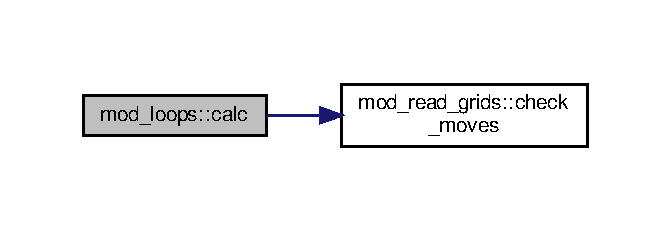
\includegraphics[width=341pt]{namespacemod__loops_a6e4de9cf9c585c364502a63d328071bd_cgraph}
\end{center}
\end{figure}


\index{mod\+\_\+loops@{mod\+\_\+loops}!calc\+\_\+ztotal@{calc\+\_\+ztotal}}
\index{calc\+\_\+ztotal@{calc\+\_\+ztotal}!mod\+\_\+loops@{mod\+\_\+loops}}
\subsubsection[{\texorpdfstring{calc\+\_\+ztotal}{calc_ztotal}}]{\setlength{\rightskip}{0pt plus 5cm}subroutine mod\+\_\+loops\+::calc\+\_\+ztotal (
\begin{DoxyParamCaption}
{}
\end{DoxyParamCaption}
)}\hypertarget{namespacemod__loops_acfec0f16ef59b6277e9dfd13d5026965}{}\label{namespacemod__loops_acfec0f16ef59b6277e9dfd13d5026965}


This routine performs partition function calculation for each grid point and also for the whole grid. 

\begin{DoxyAuthor}{Author}
Felippe M. Colombari
\begin{DoxyItemize}
\item Laboratório de Química Teórica, L\+QT -- U\+F\+S\+Car 
\end{DoxyItemize}
\end{DoxyAuthor}
\begin{DoxyDate}{Date}
-\/ Jun, 2017
\begin{DoxyItemize}
\item subroutine created 
\end{DoxyItemize}

-\/ Dec, 2017
\begin{DoxyItemize}
\item absolute energy values are recovered and thermodynamic properties are obtained from them 
\end{DoxyItemize}

-\/ Mar, 2019
\begin{DoxyItemize}
\item -\/\+TdS from ideal gas is subtracted from free energy 
\end{DoxyItemize}
\end{DoxyDate}


Definition at line 479 of file mod\+\_\+loops.\+f90.



References mod\+\_\+read\+\_\+grids\+::a, atotal, mod\+\_\+read\+\_\+grids\+::eavg, etotalavg, mod\+\_\+read\+\_\+grids\+::grid\+\_\+rot, mod\+\_\+read\+\_\+grids\+::grid\+\_\+trans, mod\+\_\+constants\+::kb, kbt, min\+\_\+ener, min\+\_\+ener\+\_\+t, mod\+\_\+read\+\_\+grids\+::mts, mtstotal, mod\+\_\+input\+\_\+read\+::np, mod\+\_\+read\+\_\+grids\+::probt, mod\+\_\+read\+\_\+grids\+::sumvexpvrot, sumvexpvtrans, mod\+\_\+input\+\_\+read\+::temp, mod\+\_\+read\+\_\+grids\+::vtot, mod\+\_\+read\+\_\+grids\+::zrot, and ztrans.



Referenced by themis().

\index{mod\+\_\+loops@{mod\+\_\+loops}!recalc@{recalc}}
\index{recalc@{recalc}!mod\+\_\+loops@{mod\+\_\+loops}}
\subsubsection[{\texorpdfstring{recalc}{recalc}}]{\setlength{\rightskip}{0pt plus 5cm}subroutine mod\+\_\+loops\+::recalc (
\begin{DoxyParamCaption}
{}
\end{DoxyParamCaption}
)}\hypertarget{namespacemod__loops_a755c1c6e9232a99181d4ac9a7c0c5cff}{}\label{namespacemod__loops_a755c1c6e9232a99181d4ac9a7c0c5cff}


This routine performs the main loop and reads already calculated energy values from energy file. 

\begin{DoxyAuthor}{Author}
Felippe M. Colombari
\begin{DoxyItemize}
\item Laboratório de Química Teórica, L\+QT -- U\+F\+S\+Car 
\end{DoxyItemize}
\end{DoxyAuthor}
\begin{DoxyDate}{Date}
-\/ Jun, 2017
\begin{DoxyItemize}
\item subroutine created
\item energy values read from binary file 
\end{DoxyItemize}

-\/ Dec, 2017
\begin{DoxyItemize}
\item lowest energy values are subtracted from each value to avoid problems in exponential calculation 
\end{DoxyItemize}
\end{DoxyDate}


Definition at line 335 of file mod\+\_\+loops.\+f90.



References mod\+\_\+read\+\_\+grids\+::check\+\_\+moves(), mod\+\_\+read\+\_\+grids\+::grid\+\_\+rot, mod\+\_\+read\+\_\+grids\+::grid\+\_\+trans, mod\+\_\+inquire\+::inquire\+\_\+check(), mod\+\_\+constants\+::kb, kbt, min\+\_\+ener, min\+\_\+ener\+\_\+t, mod\+\_\+input\+\_\+read\+::np, mod\+\_\+input\+\_\+read\+::potential, mod\+\_\+read\+\_\+grids\+::repulsion, mod\+\_\+read\+\_\+grids\+::sumvexpvrot, mod\+\_\+input\+\_\+read\+::temp, mod\+\_\+read\+\_\+grids\+::vtot, and mod\+\_\+read\+\_\+grids\+::zrot.



Referenced by themis().



Here is the call graph for this function\+:\nopagebreak
\begin{figure}[H]
\begin{center}
\leavevmode
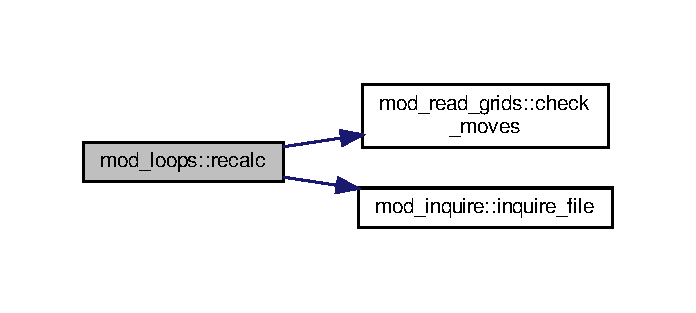
\includegraphics[width=330pt]{namespacemod__loops_a755c1c6e9232a99181d4ac9a7c0c5cff_cgraph}
\end{center}
\end{figure}




\subsection{Variable Documentation}
\index{mod\+\_\+loops@{mod\+\_\+loops}!atotal@{atotal}}
\index{atotal@{atotal}!mod\+\_\+loops@{mod\+\_\+loops}}
\subsubsection[{\texorpdfstring{atotal}{atotal}}]{\setlength{\rightskip}{0pt plus 5cm}real( kind = dp ) mod\+\_\+loops\+::atotal}\hypertarget{namespacemod__loops_a16597662d980828d74a9078f4b74e677}{}\label{namespacemod__loops_a16597662d980828d74a9078f4b74e677}


Definition at line 20 of file mod\+\_\+loops.\+f90.



Referenced by calc\+\_\+ztotal(), and mod\+\_\+resume\+::sort\+\_\+output().

\index{mod\+\_\+loops@{mod\+\_\+loops}!etotalavg@{etotalavg}}
\index{etotalavg@{etotalavg}!mod\+\_\+loops@{mod\+\_\+loops}}
\subsubsection[{\texorpdfstring{etotalavg}{etotalavg}}]{\setlength{\rightskip}{0pt plus 5cm}real( kind = dp ) mod\+\_\+loops\+::etotalavg}\hypertarget{namespacemod__loops_ad69a647146ed54f5c84b96e742396716}{}\label{namespacemod__loops_ad69a647146ed54f5c84b96e742396716}


Definition at line 20 of file mod\+\_\+loops.\+f90.



Referenced by calc\+\_\+ztotal(), and mod\+\_\+resume\+::sort\+\_\+output().

\index{mod\+\_\+loops@{mod\+\_\+loops}!kbt@{kbt}}
\index{kbt@{kbt}!mod\+\_\+loops@{mod\+\_\+loops}}
\subsubsection[{\texorpdfstring{kbt}{kbt}}]{\setlength{\rightskip}{0pt plus 5cm}real( kind = dp ) mod\+\_\+loops\+::kbt}\hypertarget{namespacemod__loops_a28f32cc48dca88b5eb914f3b51ff36c4}{}\label{namespacemod__loops_a28f32cc48dca88b5eb914f3b51ff36c4}


Definition at line 19 of file mod\+\_\+loops.\+f90.



Referenced by calc(), calc\+\_\+ztotal(), mod\+\_\+search\+::count\+\_\+structures(), recalc(), mod\+\_\+search\+::sort\+\_\+energy(), and mod\+\_\+resume\+::sort\+\_\+output().

\index{mod\+\_\+loops@{mod\+\_\+loops}!min\+\_\+ener@{min\+\_\+ener}}
\index{min\+\_\+ener@{min\+\_\+ener}!mod\+\_\+loops@{mod\+\_\+loops}}
\subsubsection[{\texorpdfstring{min\+\_\+ener}{min_ener}}]{\setlength{\rightskip}{0pt plus 5cm}real( kind = dp ) mod\+\_\+loops\+::min\+\_\+ener}\hypertarget{namespacemod__loops_a17eba688dba567d251d70c4c22d9a1cb}{}\label{namespacemod__loops_a17eba688dba567d251d70c4c22d9a1cb}


Definition at line 19 of file mod\+\_\+loops.\+f90.



Referenced by calc(), calc\+\_\+ztotal(), mod\+\_\+search\+::count\+\_\+structures(), mod\+\_\+resume\+::ending(), recalc(), mod\+\_\+search\+::sort\+\_\+energy(), and mod\+\_\+resume\+::sort\+\_\+output().

\index{mod\+\_\+loops@{mod\+\_\+loops}!min\+\_\+ener\+\_\+t@{min\+\_\+ener\+\_\+t}}
\index{min\+\_\+ener\+\_\+t@{min\+\_\+ener\+\_\+t}!mod\+\_\+loops@{mod\+\_\+loops}}
\subsubsection[{\texorpdfstring{min\+\_\+ener\+\_\+t}{min_ener_t}}]{\setlength{\rightskip}{0pt plus 5cm}real( kind = dp ), dimension(\+:), allocatable mod\+\_\+loops\+::min\+\_\+ener\+\_\+t}\hypertarget{namespacemod__loops_a285da08b33e0b132d883ee82f39f6ea2}{}\label{namespacemod__loops_a285da08b33e0b132d883ee82f39f6ea2}


Definition at line 22 of file mod\+\_\+loops.\+f90.



Referenced by calc(), calc\+\_\+ztotal(), mod\+\_\+deallocate\+\_\+all\+::deallocate\+\_\+arrays(), and recalc().

\index{mod\+\_\+loops@{mod\+\_\+loops}!mtstotal@{mtstotal}}
\index{mtstotal@{mtstotal}!mod\+\_\+loops@{mod\+\_\+loops}}
\subsubsection[{\texorpdfstring{mtstotal}{mtstotal}}]{\setlength{\rightskip}{0pt plus 5cm}real( kind = dp ) mod\+\_\+loops\+::mtstotal}\hypertarget{namespacemod__loops_ae00fd72d753b56050294575eca6b68b1}{}\label{namespacemod__loops_ae00fd72d753b56050294575eca6b68b1}


Definition at line 20 of file mod\+\_\+loops.\+f90.



Referenced by calc\+\_\+ztotal(), and mod\+\_\+resume\+::sort\+\_\+output().

\index{mod\+\_\+loops@{mod\+\_\+loops}!npre@{npre}}
\index{npre@{npre}!mod\+\_\+loops@{mod\+\_\+loops}}
\subsubsection[{\texorpdfstring{npre}{npre}}]{\setlength{\rightskip}{0pt plus 5cm}character( len = 3 ) mod\+\_\+loops\+::npre}\hypertarget{namespacemod__loops_a920fecb79f5e908fa035a810b4d549ea}{}\label{namespacemod__loops_a920fecb79f5e908fa035a810b4d549ea}


Definition at line 17 of file mod\+\_\+loops.\+f90.

\index{mod\+\_\+loops@{mod\+\_\+loops}!nrot@{nrot}}
\index{nrot@{nrot}!mod\+\_\+loops@{mod\+\_\+loops}}
\subsubsection[{\texorpdfstring{nrot}{nrot}}]{\setlength{\rightskip}{0pt plus 5cm}character( len = 3 ) mod\+\_\+loops\+::nrot}\hypertarget{namespacemod__loops_a66417533bb22418eb95ee7ebbff1f850}{}\label{namespacemod__loops_a66417533bb22418eb95ee7ebbff1f850}


Definition at line 17 of file mod\+\_\+loops.\+f90.

\index{mod\+\_\+loops@{mod\+\_\+loops}!ntra@{ntra}}
\index{ntra@{ntra}!mod\+\_\+loops@{mod\+\_\+loops}}
\subsubsection[{\texorpdfstring{ntra}{ntra}}]{\setlength{\rightskip}{0pt plus 5cm}character( len = 4 ) mod\+\_\+loops\+::ntra}\hypertarget{namespacemod__loops_a79e040eb372f8de350337242a159e2b7}{}\label{namespacemod__loops_a79e040eb372f8de350337242a159e2b7}


Definition at line 18 of file mod\+\_\+loops.\+f90.

\index{mod\+\_\+loops@{mod\+\_\+loops}!rate@{rate}}
\index{rate@{rate}!mod\+\_\+loops@{mod\+\_\+loops}}
\subsubsection[{\texorpdfstring{rate}{rate}}]{\setlength{\rightskip}{0pt plus 5cm}integer mod\+\_\+loops\+::rate}\hypertarget{namespacemod__loops_ab4cd7025ac3ba99baaa6d706f7c7cdb7}{}\label{namespacemod__loops_ab4cd7025ac3ba99baaa6d706f7c7cdb7}


Definition at line 23 of file mod\+\_\+loops.\+f90.



Referenced by calc().

\index{mod\+\_\+loops@{mod\+\_\+loops}!sumvexpvtrans@{sumvexpvtrans}}
\index{sumvexpvtrans@{sumvexpvtrans}!mod\+\_\+loops@{mod\+\_\+loops}}
\subsubsection[{\texorpdfstring{sumvexpvtrans}{sumvexpvtrans}}]{\setlength{\rightskip}{0pt plus 5cm}real( kind = dp ) mod\+\_\+loops\+::sumvexpvtrans}\hypertarget{namespacemod__loops_a7c4cc7b204cbf0459e4519befe2b1ef5}{}\label{namespacemod__loops_a7c4cc7b204cbf0459e4519befe2b1ef5}


Definition at line 21 of file mod\+\_\+loops.\+f90.



Referenced by calc\+\_\+ztotal().

\index{mod\+\_\+loops@{mod\+\_\+loops}!t0@{t0}}
\index{t0@{t0}!mod\+\_\+loops@{mod\+\_\+loops}}
\subsubsection[{\texorpdfstring{t0}{t0}}]{\setlength{\rightskip}{0pt plus 5cm}real( kind = dp ) mod\+\_\+loops\+::t0}\hypertarget{namespacemod__loops_ab6a118712ba0b676790e9cace45c35b5}{}\label{namespacemod__loops_ab6a118712ba0b676790e9cace45c35b5}


Definition at line 19 of file mod\+\_\+loops.\+f90.



Referenced by calc().

\index{mod\+\_\+loops@{mod\+\_\+loops}!tend@{tend}}
\index{tend@{tend}!mod\+\_\+loops@{mod\+\_\+loops}}
\subsubsection[{\texorpdfstring{tend}{tend}}]{\setlength{\rightskip}{0pt plus 5cm}integer mod\+\_\+loops\+::tend}\hypertarget{namespacemod__loops_a67ea99979384ac6268ae84f7bd2773ec}{}\label{namespacemod__loops_a67ea99979384ac6268ae84f7bd2773ec}


Definition at line 23 of file mod\+\_\+loops.\+f90.



Referenced by calc().

\index{mod\+\_\+loops@{mod\+\_\+loops}!time@{time}}
\index{time@{time}!mod\+\_\+loops@{mod\+\_\+loops}}
\subsubsection[{\texorpdfstring{time}{time}}]{\setlength{\rightskip}{0pt plus 5cm}real( kind = dp ) mod\+\_\+loops\+::time}\hypertarget{namespacemod__loops_acb345fb5782ee4c7fd3c419baff2c135}{}\label{namespacemod__loops_acb345fb5782ee4c7fd3c419baff2c135}


Definition at line 19 of file mod\+\_\+loops.\+f90.



Referenced by calc().

\index{mod\+\_\+loops@{mod\+\_\+loops}!tini@{tini}}
\index{tini@{tini}!mod\+\_\+loops@{mod\+\_\+loops}}
\subsubsection[{\texorpdfstring{tini}{tini}}]{\setlength{\rightskip}{0pt plus 5cm}integer mod\+\_\+loops\+::tini}\hypertarget{namespacemod__loops_adc96eb69b7265038868c81104240ee96}{}\label{namespacemod__loops_adc96eb69b7265038868c81104240ee96}


Definition at line 23 of file mod\+\_\+loops.\+f90.



Referenced by calc().

\index{mod\+\_\+loops@{mod\+\_\+loops}!ztrans@{ztrans}}
\index{ztrans@{ztrans}!mod\+\_\+loops@{mod\+\_\+loops}}
\subsubsection[{\texorpdfstring{ztrans}{ztrans}}]{\setlength{\rightskip}{0pt plus 5cm}real( kind = dp ) mod\+\_\+loops\+::ztrans}\hypertarget{namespacemod__loops_a6975a502e7bc56e3b95ee8ed8db8e658}{}\label{namespacemod__loops_a6975a502e7bc56e3b95ee8ed8db8e658}


Definition at line 21 of file mod\+\_\+loops.\+f90.



Referenced by calc\+\_\+ztotal(), mod\+\_\+search\+::sort\+\_\+energy(), and mod\+\_\+resume\+::sort\+\_\+output().


\hypertarget{namespacemod__pot__ljc}{}\section{mod\+\_\+pot\+\_\+ljc Module Reference}
\label{namespacemod__pot__ljc}\index{mod\+\_\+pot\+\_\+ljc@{mod\+\_\+pot\+\_\+ljc}}


This module performs LJ + coulombic potential calculations.  


\subsection*{Data Types}
\begin{DoxyCompactItemize}
\item 
type \hyperlink{structmod__pot__ljc_1_1dimer__ljc}{dimer\+\_\+ljc}
\item 
type \hyperlink{structmod__pot__ljc_1_1ljc__atom}{ljc\+\_\+atom}
\item 
type \hyperlink{structmod__pot__ljc_1_1ljc__mol}{ljc\+\_\+mol}
\end{DoxyCompactItemize}
\subsection*{Functions/\+Subroutines}
\begin{DoxyCompactItemize}
\item 
subroutine \hyperlink{namespacemod__pot__ljc_aba75dd17c928cdddf564bf03d18b3ee2}{read\+\_\+ljc\+\_\+params} (this, ljc\+\_\+filename, numat)
\begin{DoxyCompactList}\small\item\em This routine reads atom names, charges, sigma and epsilon values from parameter files. \end{DoxyCompactList}\item 
subroutine \hyperlink{namespacemod__pot__ljc_ae251ed7b35f9a6401200390d8684ea46}{check\+\_\+ljc\+\_\+params} (this, numat)
\begin{DoxyCompactList}\small\item\em This routine checks for inconsistent entries on parameter files. \end{DoxyCompactList}\item 
subroutine \hyperlink{namespacemod__pot__ljc_aea69edf70ec804ebb8075741c84ab50b}{calc\+\_\+ljc\+\_\+cross} (this)
\begin{DoxyCompactList}\small\item\em This routine calculates crossing values for LJ + coulomb potential before the loops. \end{DoxyCompactList}\item 
subroutine \hyperlink{namespacemod__pot__ljc_a13c36fde6ac0af7265630bc8105c23b6}{calc\+\_\+ljc\+\_\+energy} (this, p, r, t)
\begin{DoxyCompactList}\small\item\em This routine calculates LJ + coulomb energy for each valid configuration. \end{DoxyCompactList}\end{DoxyCompactItemize}
\subsection*{Variables}
\begin{DoxyCompactItemize}
\item 
type(\hyperlink{structmod__pot__ljc_1_1ljc__mol}{ljc\+\_\+mol}) \hyperlink{namespacemod__pot__ljc_a840c66fc49efca8db3e2c54932a77356}{mol1\+\_\+ljc}
\item 
type(\hyperlink{structmod__pot__ljc_1_1ljc__mol}{ljc\+\_\+mol}) \hyperlink{namespacemod__pot__ljc_a2b003eb4461125a250324cf11fdd50c7}{mol2\+\_\+ljc}
\item 
type(\hyperlink{structmod__pot__ljc_1_1dimer__ljc}{dimer\+\_\+ljc}) \hyperlink{namespacemod__pot__ljc_abbcaeaac6c53085e893805852918464d}{dimer}
\end{DoxyCompactItemize}


\subsection{Detailed Description}
This module performs LJ + coulombic potential calculations. 

\begin{DoxyAuthor}{Author}
Felippe M. Colombari
\begin{DoxyItemize}
\item Laboratório de Química Teórica, L\+QT -- U\+F\+S\+Car 
\end{DoxyItemize}
\end{DoxyAuthor}
\begin{DoxyDate}{Date}
-\/ Oct, 2017
\begin{DoxyItemize}
\item module created 
\end{DoxyItemize}
\end{DoxyDate}


\subsection{Function/\+Subroutine Documentation}
\index{mod\+\_\+pot\+\_\+ljc@{mod\+\_\+pot\+\_\+ljc}!calc\+\_\+ljc\+\_\+cross@{calc\+\_\+ljc\+\_\+cross}}
\index{calc\+\_\+ljc\+\_\+cross@{calc\+\_\+ljc\+\_\+cross}!mod\+\_\+pot\+\_\+ljc@{mod\+\_\+pot\+\_\+ljc}}
\subsubsection[{\texorpdfstring{calc\+\_\+ljc\+\_\+cross(this)}{calc_ljc_cross(this)}}]{\setlength{\rightskip}{0pt plus 5cm}subroutine mod\+\_\+pot\+\_\+ljc\+::calc\+\_\+ljc\+\_\+cross (
\begin{DoxyParamCaption}
\item[{class( {\bf dimer\+\_\+ljc} ), intent(inout)}]{this}
\end{DoxyParamCaption}
)}\hypertarget{namespacemod__pot__ljc_aea69edf70ec804ebb8075741c84ab50b}{}\label{namespacemod__pot__ljc_aea69edf70ec804ebb8075741c84ab50b}


This routine calculates crossing values for LJ + coulomb potential before the loops. 

\begin{DoxyAuthor}{Author}
Felippe M. Colombari 
\end{DoxyAuthor}


Definition at line 139 of file mod\+\_\+pot\+\_\+ljc.\+f90.



References mod\+\_\+read\+\_\+xyz\+::mol1, mol1\+\_\+ljc, mod\+\_\+read\+\_\+xyz\+::mol2, and mol2\+\_\+ljc.

\index{mod\+\_\+pot\+\_\+ljc@{mod\+\_\+pot\+\_\+ljc}!calc\+\_\+ljc\+\_\+energy@{calc\+\_\+ljc\+\_\+energy}}
\index{calc\+\_\+ljc\+\_\+energy@{calc\+\_\+ljc\+\_\+energy}!mod\+\_\+pot\+\_\+ljc@{mod\+\_\+pot\+\_\+ljc}}
\subsubsection[{\texorpdfstring{calc\+\_\+ljc\+\_\+energy(this, p, r, t)}{calc_ljc_energy(this, p, r, t)}}]{\setlength{\rightskip}{0pt plus 5cm}subroutine mod\+\_\+pot\+\_\+ljc\+::calc\+\_\+ljc\+\_\+energy (
\begin{DoxyParamCaption}
\item[{class( {\bf dimer\+\_\+ljc} ), intent(inout)}]{this, }
\item[{integer, intent(in)}]{p, }
\item[{integer, intent(in)}]{r, }
\item[{integer, intent(in)}]{t}
\end{DoxyParamCaption}
)}\hypertarget{namespacemod__pot__ljc_a13c36fde6ac0af7265630bc8105c23b6}{}\label{namespacemod__pot__ljc_a13c36fde6ac0af7265630bc8105c23b6}


This routine calculates LJ + coulomb energy for each valid configuration. 

\begin{DoxyAuthor}{Author}
Felippe M. Colombari 
\end{DoxyAuthor}


Definition at line 176 of file mod\+\_\+pot\+\_\+ljc.\+f90.



References mod\+\_\+constants\+::ccon, mod\+\_\+read\+\_\+xyz\+::mol1, mod\+\_\+read\+\_\+xyz\+::mol2, mod\+\_\+input\+\_\+read\+::rcut\+\_\+sqr, mod\+\_\+read\+\_\+grids\+::repulsion, and mod\+\_\+read\+\_\+grids\+::vtot.

\index{mod\+\_\+pot\+\_\+ljc@{mod\+\_\+pot\+\_\+ljc}!check\+\_\+ljc\+\_\+params@{check\+\_\+ljc\+\_\+params}}
\index{check\+\_\+ljc\+\_\+params@{check\+\_\+ljc\+\_\+params}!mod\+\_\+pot\+\_\+ljc@{mod\+\_\+pot\+\_\+ljc}}
\subsubsection[{\texorpdfstring{check\+\_\+ljc\+\_\+params(this, numat)}{check_ljc_params(this, numat)}}]{\setlength{\rightskip}{0pt plus 5cm}subroutine mod\+\_\+pot\+\_\+ljc\+::check\+\_\+ljc\+\_\+params (
\begin{DoxyParamCaption}
\item[{class( {\bf ljc\+\_\+mol} ), intent(inout)}]{this, }
\item[{integer, intent(in)}]{numat}
\end{DoxyParamCaption}
)}\hypertarget{namespacemod__pot__ljc_ae251ed7b35f9a6401200390d8684ea46}{}\label{namespacemod__pot__ljc_ae251ed7b35f9a6401200390d8684ea46}


This routine checks for inconsistent entries on parameter files. 

\begin{DoxyAuthor}{Author}
Felippe M. Colombari 
\end{DoxyAuthor}


Definition at line 96 of file mod\+\_\+pot\+\_\+ljc.\+f90.



References mod\+\_\+constants\+::dashline.

\index{mod\+\_\+pot\+\_\+ljc@{mod\+\_\+pot\+\_\+ljc}!read\+\_\+ljc\+\_\+params@{read\+\_\+ljc\+\_\+params}}
\index{read\+\_\+ljc\+\_\+params@{read\+\_\+ljc\+\_\+params}!mod\+\_\+pot\+\_\+ljc@{mod\+\_\+pot\+\_\+ljc}}
\subsubsection[{\texorpdfstring{read\+\_\+ljc\+\_\+params(this, ljc\+\_\+filename, numat)}{read_ljc_params(this, ljc_filename, numat)}}]{\setlength{\rightskip}{0pt plus 5cm}subroutine mod\+\_\+pot\+\_\+ljc\+::read\+\_\+ljc\+\_\+params (
\begin{DoxyParamCaption}
\item[{class( {\bf ljc\+\_\+mol} ), intent(inout)}]{this, }
\item[{character( len = $\ast$ ), intent(in)}]{ljc\+\_\+filename, }
\item[{integer, intent(in)}]{numat}
\end{DoxyParamCaption}
)}\hypertarget{namespacemod__pot__ljc_aba75dd17c928cdddf564bf03d18b3ee2}{}\label{namespacemod__pot__ljc_aba75dd17c928cdddf564bf03d18b3ee2}


This routine reads atom names, charges, sigma and epsilon values from parameter files. 

\begin{DoxyAuthor}{Author}
Felippe M. Colombari 
\end{DoxyAuthor}


Definition at line 48 of file mod\+\_\+pot\+\_\+ljc.\+f90.



References mod\+\_\+inquire\+::inquire\+\_\+check().



Here is the call graph for this function\+:\nopagebreak
\begin{figure}[H]
\begin{center}
\leavevmode
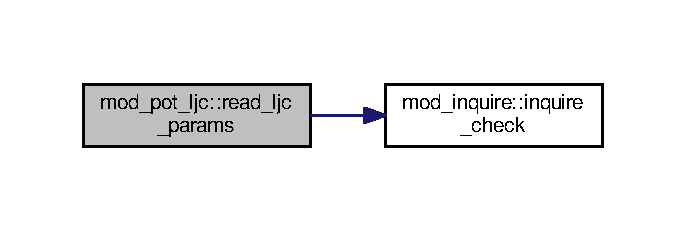
\includegraphics[width=329pt]{namespacemod__pot__ljc_aba75dd17c928cdddf564bf03d18b3ee2_cgraph}
\end{center}
\end{figure}




\subsection{Variable Documentation}
\index{mod\+\_\+pot\+\_\+ljc@{mod\+\_\+pot\+\_\+ljc}!dimer@{dimer}}
\index{dimer@{dimer}!mod\+\_\+pot\+\_\+ljc@{mod\+\_\+pot\+\_\+ljc}}
\subsubsection[{\texorpdfstring{dimer}{dimer}}]{\setlength{\rightskip}{0pt plus 5cm}type( {\bf dimer\+\_\+ljc} ) mod\+\_\+pot\+\_\+ljc\+::dimer}\hypertarget{namespacemod__pot__ljc_abbcaeaac6c53085e893805852918464d}{}\label{namespacemod__pot__ljc_abbcaeaac6c53085e893805852918464d}


Definition at line 39 of file mod\+\_\+pot\+\_\+ljc.\+f90.



Referenced by mod\+\_\+loops\+::calc(), and mod\+\_\+deallocate\+\_\+all\+::deallocate\+\_\+arrays().

\index{mod\+\_\+pot\+\_\+ljc@{mod\+\_\+pot\+\_\+ljc}!mol1\+\_\+ljc@{mol1\+\_\+ljc}}
\index{mol1\+\_\+ljc@{mol1\+\_\+ljc}!mod\+\_\+pot\+\_\+ljc@{mod\+\_\+pot\+\_\+ljc}}
\subsubsection[{\texorpdfstring{mol1\+\_\+ljc}{mol1_ljc}}]{\setlength{\rightskip}{0pt plus 5cm}type( {\bf ljc\+\_\+mol} ) mod\+\_\+pot\+\_\+ljc\+::mol1\+\_\+ljc}\hypertarget{namespacemod__pot__ljc_a840c66fc49efca8db3e2c54932a77356}{}\label{namespacemod__pot__ljc_a840c66fc49efca8db3e2c54932a77356}


Definition at line 29 of file mod\+\_\+pot\+\_\+ljc.\+f90.



Referenced by mod\+\_\+loops\+::calc(), calc\+\_\+ljc\+\_\+cross(), and mod\+\_\+deallocate\+\_\+all\+::deallocate\+\_\+arrays().

\index{mod\+\_\+pot\+\_\+ljc@{mod\+\_\+pot\+\_\+ljc}!mol2\+\_\+ljc@{mol2\+\_\+ljc}}
\index{mol2\+\_\+ljc@{mol2\+\_\+ljc}!mod\+\_\+pot\+\_\+ljc@{mod\+\_\+pot\+\_\+ljc}}
\subsubsection[{\texorpdfstring{mol2\+\_\+ljc}{mol2_ljc}}]{\setlength{\rightskip}{0pt plus 5cm}type( {\bf ljc\+\_\+mol} ) mod\+\_\+pot\+\_\+ljc\+::mol2\+\_\+ljc}\hypertarget{namespacemod__pot__ljc_a2b003eb4461125a250324cf11fdd50c7}{}\label{namespacemod__pot__ljc_a2b003eb4461125a250324cf11fdd50c7}


Definition at line 29 of file mod\+\_\+pot\+\_\+ljc.\+f90.



Referenced by mod\+\_\+loops\+::calc(), calc\+\_\+ljc\+\_\+cross(), and mod\+\_\+deallocate\+\_\+all\+::deallocate\+\_\+arrays().


\hypertarget{namespacemod__pot__none}{}\section{mod\+\_\+pot\+\_\+none Module Reference}
\label{namespacemod__pot__none}\index{mod\+\_\+pot\+\_\+none@{mod\+\_\+pot\+\_\+none}}


This module performs interatomic distance calculations when no potential is selected.  


\subsection*{Functions/\+Subroutines}
\begin{DoxyCompactItemize}
\item 
subroutine \hyperlink{namespacemod__pot__none_a696314c32ed889a4ff2b669fcacaf471}{check\+\_\+conf} (p, r, t)
\end{DoxyCompactItemize}


\subsection{Detailed Description}
This module performs interatomic distance calculations when no potential is selected. 

\begin{DoxyAuthor}{Author}
Felippe M. Colombari
\begin{DoxyItemize}
\item Laboratório de Química Teórica, L\+QT -- U\+F\+S\+Car 
\end{DoxyItemize}
\end{DoxyAuthor}
\begin{DoxyDate}{Date}
-\/ Jan, 2018
\begin{DoxyItemize}
\item module created and documented 
\end{DoxyItemize}
\end{DoxyDate}


\subsection{Function/\+Subroutine Documentation}
\index{mod\+\_\+pot\+\_\+none@{mod\+\_\+pot\+\_\+none}!check\+\_\+conf@{check\+\_\+conf}}
\index{check\+\_\+conf@{check\+\_\+conf}!mod\+\_\+pot\+\_\+none@{mod\+\_\+pot\+\_\+none}}
\subsubsection[{\texorpdfstring{check\+\_\+conf(p, r, t)}{check_conf(p, r, t)}}]{\setlength{\rightskip}{0pt plus 5cm}subroutine mod\+\_\+pot\+\_\+none\+::check\+\_\+conf (
\begin{DoxyParamCaption}
\item[{integer, intent(in)}]{p, }
\item[{integer, intent(in)}]{r, }
\item[{integer, intent(in)}]{t}
\end{DoxyParamCaption}
)}\hypertarget{namespacemod__pot__none_a696314c32ed889a4ff2b669fcacaf471}{}\label{namespacemod__pot__none_a696314c32ed889a4ff2b669fcacaf471}


Definition at line 24 of file mod\+\_\+pot\+\_\+none.\+f90.



References mod\+\_\+read\+\_\+xyz\+::mol1, mod\+\_\+read\+\_\+xyz\+::mol2, mod\+\_\+input\+\_\+read\+::rcut\+\_\+sqr, and mod\+\_\+read\+\_\+grids\+::repulsion.



Referenced by mod\+\_\+loops\+::calc().


\hypertarget{namespacemod__read__grids}{}\section{mod\+\_\+read\+\_\+grids Module Reference}
\label{namespacemod__read__grids}\index{mod\+\_\+read\+\_\+grids@{mod\+\_\+read\+\_\+grids}}


This module reads coordinate files for translation and rotation grids.  


\subsection*{Data Types}
\begin{DoxyCompactItemize}
\item 
type \hyperlink{structmod__read__grids_1_1grid}{grid}
\item 
type \hyperlink{structmod__read__grids_1_1point}{point}
\end{DoxyCompactItemize}
\subsection*{Functions/\+Subroutines}
\begin{DoxyCompactItemize}
\item 
subroutine \hyperlink{namespacemod__read__grids_af6cb0bee8e3eb7dfbaa4621275b29fa2}{read\+\_\+translation\+\_\+grid}
\begin{DoxyCompactList}\small\item\em This routine reads coordinates for user-\/defined translation grid. \end{DoxyCompactList}\item 
subroutine \hyperlink{namespacemod__read__grids_abba14a1f750b2c342d5c5a80be803310}{build\+\_\+translation\+\_\+sphere}
\item 
subroutine \hyperlink{namespacemod__read__grids_ae4fb4c515f1f9f5edd3785ca0f509ea4}{build\+\_\+rotation\+\_\+sphere}
\item 
subroutine \hyperlink{namespacemod__read__grids_a1e081c6668bb3ea97788ffe4a74f39db}{center\+\_\+translation\+\_\+grid}
\begin{DoxyCompactList}\small\item\em This routine centers user-\/defined translation grid altogether with mol1. \end{DoxyCompactList}\item 
subroutine \hyperlink{namespacemod__read__grids_a318177c120a409fe4cef7d1785b626ac}{check\+\_\+moves}
\begin{DoxyCompactList}\small\item\em This routine prints some checking information on screen. \end{DoxyCompactList}\end{DoxyCompactItemize}
\subsection*{Variables}
\begin{DoxyCompactItemize}
\item 
type(\hyperlink{structmod__read__grids_1_1grid}{grid}) \hyperlink{namespacemod__read__grids_ab09110371e13fa11f9a839bde8da8fc7}{grid\+\_\+trans}
\item 
type(\hyperlink{structmod__read__grids_1_1grid}{grid}) \hyperlink{namespacemod__read__grids_a0e370bf7268cf2484361751a7c2cbee5}{grid\+\_\+rot}
\item 
real(kind=dp), dimension(\+:), allocatable \hyperlink{namespacemod__read__grids_a1cd0dd1119fe3ce58917bf6aaf7abebf}{a}
\item 
real(kind=dp), dimension(\+:), allocatable \hyperlink{namespacemod__read__grids_af619057af0e7ce4717a95d4239422912}{mts}
\item 
real(kind=dp), dimension(\+:), allocatable \hyperlink{namespacemod__read__grids_af9747d65a3c7dd6876ab803f0a06e8e9}{eavg}
\item 
real(kind=dp), dimension(\+:), allocatable \hyperlink{namespacemod__read__grids_aa1dc0d4a91ccebc952bde4d1f380b174}{zrot}
\item 
real(kind=dp), dimension(\+:), allocatable \hyperlink{namespacemod__read__grids_aff025afae6b2b208286c65a85cd8f82a}{sumvexpvrot}
\item 
real(kind=dp), dimension(\+:), allocatable \hyperlink{namespacemod__read__grids_a019fc7a33467abb84318794f59bff9cd}{probt}
\item 
real(kind=dp), dimension(\+:), allocatable \hyperlink{namespacemod__read__grids_a668db35acd10bd5a0c686c3ea19da6c2}{rr}
\item 
real(kind=dp), dimension(\+:), allocatable \hyperlink{namespacemod__read__grids_a40918dc75ea77a2757ea8d8dd43beb9e}{thetar}
\item 
real(kind=dp), dimension(\+:), allocatable \hyperlink{namespacemod__read__grids_aa3da94e35a501dc0ed782d7019127514}{phir}
\item 
real(kind=dp), dimension(\+:,\+:,\+:), allocatable \hyperlink{namespacemod__read__grids_a1acebe9f23427d5bc54629463ab63378}{vtot}
\item 
logical, dimension(\+:,\+:,\+:), allocatable \hyperlink{namespacemod__read__grids_a78b7a722975e665430c061c6cca83ca0}{repulsion}
\item 
integer \hyperlink{namespacemod__read__grids_aa54b9eaa554b8519d41c5e616479d343}{ntotal}
\item 
integer \hyperlink{namespacemod__read__grids_aca954e32e5f53302912f372a99affe97}{rot\+\_\+total}
\end{DoxyCompactItemize}


\subsection{Detailed Description}
This module reads coordinate files for translation and rotation grids. 

\begin{DoxyAuthor}{Author}
Felippe M. Colombari
\begin{DoxyItemize}
\item Laboratório de Química Teórica, L\+QT -- U\+F\+S\+Car 
\end{DoxyItemize}
\end{DoxyAuthor}
\begin{DoxyDate}{Date}
-\/ Jan, 2018
\begin{DoxyItemize}
\item independent module created 
\end{DoxyItemize}

-\/ Jan, 2018
\begin{DoxyItemize}
\item documentation and support added 
\end{DoxyItemize}
\end{DoxyDate}
\begin{DoxyNote}{Note}

\begin{DoxyItemize}
\item grids are standard X\+YZ coordinate files. 
\end{DoxyItemize}
\end{DoxyNote}


\subsection{Function/\+Subroutine Documentation}
\index{mod\+\_\+read\+\_\+grids@{mod\+\_\+read\+\_\+grids}!build\+\_\+rotation\+\_\+sphere@{build\+\_\+rotation\+\_\+sphere}}
\index{build\+\_\+rotation\+\_\+sphere@{build\+\_\+rotation\+\_\+sphere}!mod\+\_\+read\+\_\+grids@{mod\+\_\+read\+\_\+grids}}
\subsubsection[{\texorpdfstring{build\+\_\+rotation\+\_\+sphere}{build_rotation_sphere}}]{\setlength{\rightskip}{0pt plus 5cm}subroutine mod\+\_\+read\+\_\+grids\+::build\+\_\+rotation\+\_\+sphere (
\begin{DoxyParamCaption}
{}
\end{DoxyParamCaption}
)}\hypertarget{namespacemod__read__grids_ae4fb4c515f1f9f5edd3785ca0f509ea4}{}\label{namespacemod__read__grids_ae4fb4c515f1f9f5edd3785ca0f509ea4}


Definition at line 150 of file mod\+\_\+read\+\_\+grids.\+f90.



References grid\+\_\+rot, phir, mod\+\_\+input\+\_\+read\+::rot\+\_\+factor, rr, mod\+\_\+spherical\+\_\+grids\+::sphere\+\_\+icos1\+\_\+points(), and thetar.



Referenced by themis().



Here is the call graph for this function\+:\nopagebreak
\begin{figure}[H]
\begin{center}
\leavevmode
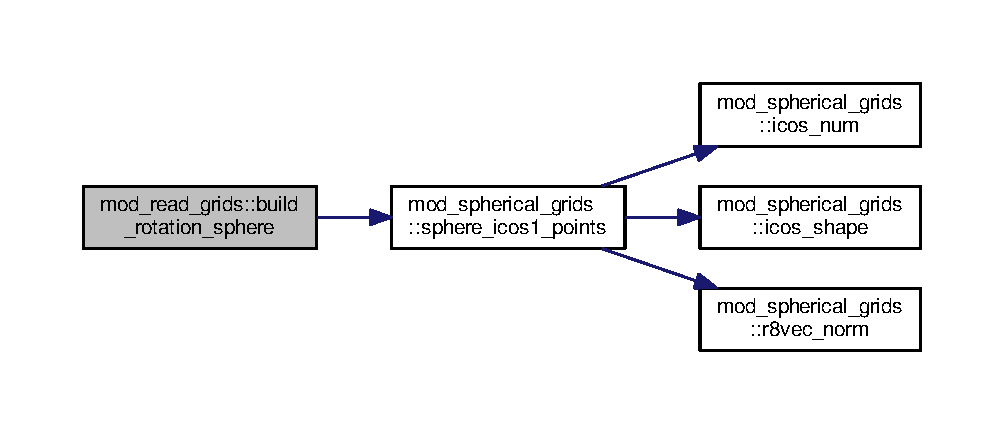
\includegraphics[width=350pt]{namespacemod__read__grids_ae4fb4c515f1f9f5edd3785ca0f509ea4_cgraph}
\end{center}
\end{figure}


\index{mod\+\_\+read\+\_\+grids@{mod\+\_\+read\+\_\+grids}!build\+\_\+translation\+\_\+sphere@{build\+\_\+translation\+\_\+sphere}}
\index{build\+\_\+translation\+\_\+sphere@{build\+\_\+translation\+\_\+sphere}!mod\+\_\+read\+\_\+grids@{mod\+\_\+read\+\_\+grids}}
\subsubsection[{\texorpdfstring{build\+\_\+translation\+\_\+sphere}{build_translation_sphere}}]{\setlength{\rightskip}{0pt plus 5cm}subroutine mod\+\_\+read\+\_\+grids\+::build\+\_\+translation\+\_\+sphere (
\begin{DoxyParamCaption}
{}
\end{DoxyParamCaption}
)}\hypertarget{namespacemod__read__grids_abba14a1f750b2c342d5c5a80be803310}{}\label{namespacemod__read__grids_abba14a1f750b2c342d5c5a80be803310}


Definition at line 118 of file mod\+\_\+read\+\_\+grids.\+f90.



References grid\+\_\+trans, mod\+\_\+cmd\+\_\+line\+::rad, mod\+\_\+spherical\+\_\+grids\+::sphere\+\_\+icos1\+\_\+points(), and mod\+\_\+input\+\_\+read\+::trans\+\_\+factor.



Referenced by themis().



Here is the call graph for this function\+:\nopagebreak
\begin{figure}[H]
\begin{center}
\leavevmode
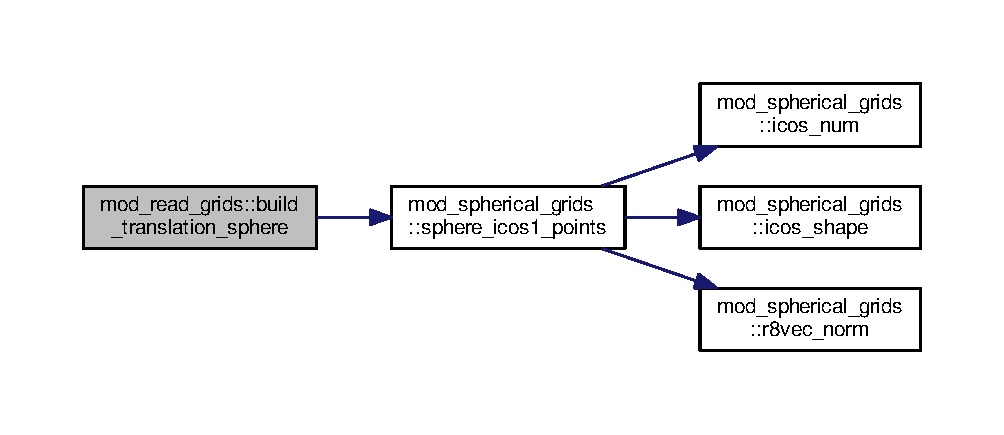
\includegraphics[width=350pt]{namespacemod__read__grids_abba14a1f750b2c342d5c5a80be803310_cgraph}
\end{center}
\end{figure}


\index{mod\+\_\+read\+\_\+grids@{mod\+\_\+read\+\_\+grids}!center\+\_\+translation\+\_\+grid@{center\+\_\+translation\+\_\+grid}}
\index{center\+\_\+translation\+\_\+grid@{center\+\_\+translation\+\_\+grid}!mod\+\_\+read\+\_\+grids@{mod\+\_\+read\+\_\+grids}}
\subsubsection[{\texorpdfstring{center\+\_\+translation\+\_\+grid}{center_translation_grid}}]{\setlength{\rightskip}{0pt plus 5cm}subroutine mod\+\_\+read\+\_\+grids\+::center\+\_\+translation\+\_\+grid (
\begin{DoxyParamCaption}
{}
\end{DoxyParamCaption}
)}\hypertarget{namespacemod__read__grids_a1e081c6668bb3ea97788ffe4a74f39db}{}\label{namespacemod__read__grids_a1e081c6668bb3ea97788ffe4a74f39db}


This routine centers user-\/defined translation grid altogether with mol1. 

\begin{DoxyAuthor}{Author}
Felippe M. Colombari
\begin{DoxyItemize}
\item Laboratório de Química Teórica, L\+QT -- U\+F\+S\+Car 
\end{DoxyItemize}
\end{DoxyAuthor}


Definition at line 226 of file mod\+\_\+read\+\_\+grids.\+f90.



References grid\+\_\+trans, mod\+\_\+read\+\_\+xyz\+::mol1, and mod\+\_\+input\+\_\+read\+::ref1.



Referenced by read\+\_\+translation\+\_\+grid().

\index{mod\+\_\+read\+\_\+grids@{mod\+\_\+read\+\_\+grids}!check\+\_\+moves@{check\+\_\+moves}}
\index{check\+\_\+moves@{check\+\_\+moves}!mod\+\_\+read\+\_\+grids@{mod\+\_\+read\+\_\+grids}}
\subsubsection[{\texorpdfstring{check\+\_\+moves}{check_moves}}]{\setlength{\rightskip}{0pt plus 5cm}subroutine mod\+\_\+read\+\_\+grids\+::check\+\_\+moves (
\begin{DoxyParamCaption}
{}
\end{DoxyParamCaption}
)}\hypertarget{namespacemod__read__grids_a318177c120a409fe4cef7d1785b626ac}{}\label{namespacemod__read__grids_a318177c120a409fe4cef7d1785b626ac}


This routine prints some checking information on screen. 

\begin{DoxyAuthor}{Author}
Felippe M. Colombari
\begin{DoxyItemize}
\item Laboratório de Química Teórica, L\+QT -- U\+F\+S\+Car 
\end{DoxyItemize}
\end{DoxyAuthor}
\begin{DoxyDate}{Date}
-\/ Dec, 2017
\begin{DoxyItemize}
\item subroutine created and documented 
\end{DoxyItemize}
\end{DoxyDate}


Definition at line 260 of file mod\+\_\+read\+\_\+grids.\+f90.



References mod\+\_\+constants\+::dashline, grid\+\_\+rot, grid\+\_\+trans, mod\+\_\+input\+\_\+read\+::maxp, mod\+\_\+input\+\_\+read\+::np, ntotal, and rot\+\_\+total.



Referenced by mod\+\_\+loops\+::calc(), and mod\+\_\+loops\+::recalc().

\index{mod\+\_\+read\+\_\+grids@{mod\+\_\+read\+\_\+grids}!read\+\_\+translation\+\_\+grid@{read\+\_\+translation\+\_\+grid}}
\index{read\+\_\+translation\+\_\+grid@{read\+\_\+translation\+\_\+grid}!mod\+\_\+read\+\_\+grids@{mod\+\_\+read\+\_\+grids}}
\subsubsection[{\texorpdfstring{read\+\_\+translation\+\_\+grid}{read_translation_grid}}]{\setlength{\rightskip}{0pt plus 5cm}subroutine mod\+\_\+read\+\_\+grids\+::read\+\_\+translation\+\_\+grid (
\begin{DoxyParamCaption}
{}
\end{DoxyParamCaption}
)}\hypertarget{namespacemod__read__grids_af6cb0bee8e3eb7dfbaa4621275b29fa2}{}\label{namespacemod__read__grids_af6cb0bee8e3eb7dfbaa4621275b29fa2}


This routine reads coordinates for user-\/defined translation grid. 

\begin{DoxyAuthor}{Author}
Felippe M. Colombari
\begin{DoxyItemize}
\item Laboratório de Química Teórica, L\+QT -- U\+F\+S\+Car 
\end{DoxyItemize}
\end{DoxyAuthor}
\begin{DoxyDate}{Date}
-\/ Jun, 2017
\begin{DoxyItemize}
\item first version 
\end{DoxyItemize}

-\/ Dec, 2017
\begin{DoxyItemize}
\item modular subroutine created 
\end{DoxyItemize}

-\/ Jan, 2018
\begin{DoxyItemize}
\item final version, documentation and support 
\end{DoxyItemize}
\end{DoxyDate}


Definition at line 55 of file mod\+\_\+read\+\_\+grids.\+f90.



References center\+\_\+translation\+\_\+grid(), grid\+\_\+trans, mod\+\_\+cmd\+\_\+line\+::grid\+\_\+transl, and mod\+\_\+inquire\+::inquire\+\_\+check().



Referenced by themis().



Here is the call graph for this function\+:\nopagebreak
\begin{figure}[H]
\begin{center}
\leavevmode
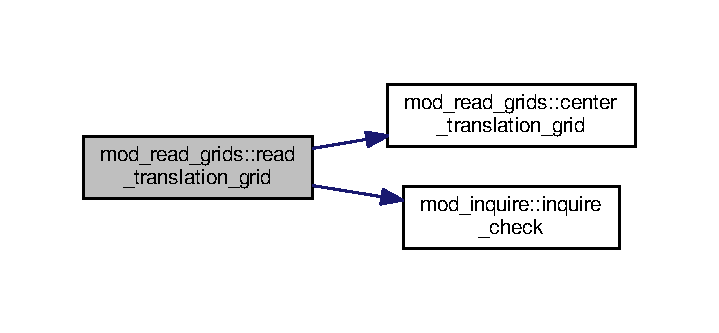
\includegraphics[width=345pt]{namespacemod__read__grids_af6cb0bee8e3eb7dfbaa4621275b29fa2_cgraph}
\end{center}
\end{figure}




\subsection{Variable Documentation}
\index{mod\+\_\+read\+\_\+grids@{mod\+\_\+read\+\_\+grids}!a@{a}}
\index{a@{a}!mod\+\_\+read\+\_\+grids@{mod\+\_\+read\+\_\+grids}}
\subsubsection[{\texorpdfstring{a}{a}}]{\setlength{\rightskip}{0pt plus 5cm}real( kind = dp ), dimension(\+:), allocatable mod\+\_\+read\+\_\+grids\+::a}\hypertarget{namespacemod__read__grids_a1cd0dd1119fe3ce58917bf6aaf7abebf}{}\label{namespacemod__read__grids_a1cd0dd1119fe3ce58917bf6aaf7abebf}


Definition at line 33 of file mod\+\_\+read\+\_\+grids.\+f90.



Referenced by mod\+\_\+loops\+::calc\+\_\+ztotal(), mod\+\_\+resume\+::ending(), mod\+\_\+resume\+::sort\+\_\+output(), and mod\+\_\+vmd\+::write\+\_\+vmd\+\_\+files().

\index{mod\+\_\+read\+\_\+grids@{mod\+\_\+read\+\_\+grids}!eavg@{eavg}}
\index{eavg@{eavg}!mod\+\_\+read\+\_\+grids@{mod\+\_\+read\+\_\+grids}}
\subsubsection[{\texorpdfstring{eavg}{eavg}}]{\setlength{\rightskip}{0pt plus 5cm}real( kind = dp ), dimension(\+:), allocatable mod\+\_\+read\+\_\+grids\+::eavg}\hypertarget{namespacemod__read__grids_af9747d65a3c7dd6876ab803f0a06e8e9}{}\label{namespacemod__read__grids_af9747d65a3c7dd6876ab803f0a06e8e9}


Definition at line 33 of file mod\+\_\+read\+\_\+grids.\+f90.



Referenced by mod\+\_\+loops\+::calc\+\_\+ztotal(), mod\+\_\+resume\+::sort\+\_\+output(), and mod\+\_\+vmd\+::write\+\_\+vmd\+\_\+files().

\index{mod\+\_\+read\+\_\+grids@{mod\+\_\+read\+\_\+grids}!grid\+\_\+rot@{grid\+\_\+rot}}
\index{grid\+\_\+rot@{grid\+\_\+rot}!mod\+\_\+read\+\_\+grids@{mod\+\_\+read\+\_\+grids}}
\subsubsection[{\texorpdfstring{grid\+\_\+rot}{grid_rot}}]{\setlength{\rightskip}{0pt plus 5cm}type( {\bf grid} ) mod\+\_\+read\+\_\+grids\+::grid\+\_\+rot}\hypertarget{namespacemod__read__grids_a0e370bf7268cf2484361751a7c2cbee5}{}\label{namespacemod__read__grids_a0e370bf7268cf2484361751a7c2cbee5}


Definition at line 31 of file mod\+\_\+read\+\_\+grids.\+f90.



Referenced by build\+\_\+rotation\+\_\+sphere(), mod\+\_\+loops\+::calc(), mod\+\_\+loops\+::calc\+\_\+ztotal(), check\+\_\+moves(), mod\+\_\+search\+::count\+\_\+structures(), mod\+\_\+deallocate\+\_\+all\+::deallocate\+\_\+arrays(), mod\+\_\+loops\+::recalc(), and mod\+\_\+search\+::search\+\_\+structures().

\index{mod\+\_\+read\+\_\+grids@{mod\+\_\+read\+\_\+grids}!grid\+\_\+trans@{grid\+\_\+trans}}
\index{grid\+\_\+trans@{grid\+\_\+trans}!mod\+\_\+read\+\_\+grids@{mod\+\_\+read\+\_\+grids}}
\subsubsection[{\texorpdfstring{grid\+\_\+trans}{grid_trans}}]{\setlength{\rightskip}{0pt plus 5cm}type( {\bf grid} ) mod\+\_\+read\+\_\+grids\+::grid\+\_\+trans}\hypertarget{namespacemod__read__grids_ab09110371e13fa11f9a839bde8da8fc7}{}\label{namespacemod__read__grids_ab09110371e13fa11f9a839bde8da8fc7}


Definition at line 31 of file mod\+\_\+read\+\_\+grids.\+f90.



Referenced by build\+\_\+translation\+\_\+sphere(), mod\+\_\+loops\+::calc(), mod\+\_\+loops\+::calc\+\_\+ztotal(), center\+\_\+translation\+\_\+grid(), check\+\_\+moves(), mod\+\_\+search\+::count\+\_\+structures(), mod\+\_\+deallocate\+\_\+all\+::deallocate\+\_\+arrays(), read\+\_\+translation\+\_\+grid(), mod\+\_\+loops\+::recalc(), mod\+\_\+search\+::search\+\_\+structures(), and mod\+\_\+resume\+::sort\+\_\+output().

\index{mod\+\_\+read\+\_\+grids@{mod\+\_\+read\+\_\+grids}!mts@{mts}}
\index{mts@{mts}!mod\+\_\+read\+\_\+grids@{mod\+\_\+read\+\_\+grids}}
\subsubsection[{\texorpdfstring{mts}{mts}}]{\setlength{\rightskip}{0pt plus 5cm}real( kind = dp ), dimension(\+:), allocatable mod\+\_\+read\+\_\+grids\+::mts}\hypertarget{namespacemod__read__grids_af619057af0e7ce4717a95d4239422912}{}\label{namespacemod__read__grids_af619057af0e7ce4717a95d4239422912}


Definition at line 33 of file mod\+\_\+read\+\_\+grids.\+f90.



Referenced by mod\+\_\+loops\+::calc\+\_\+ztotal(), mod\+\_\+resume\+::sort\+\_\+output(), and mod\+\_\+vmd\+::write\+\_\+vmd\+\_\+files().

\index{mod\+\_\+read\+\_\+grids@{mod\+\_\+read\+\_\+grids}!ntotal@{ntotal}}
\index{ntotal@{ntotal}!mod\+\_\+read\+\_\+grids@{mod\+\_\+read\+\_\+grids}}
\subsubsection[{\texorpdfstring{ntotal}{ntotal}}]{\setlength{\rightskip}{0pt plus 5cm}integer mod\+\_\+read\+\_\+grids\+::ntotal}\hypertarget{namespacemod__read__grids_aa54b9eaa554b8519d41c5e616479d343}{}\label{namespacemod__read__grids_aa54b9eaa554b8519d41c5e616479d343}


Definition at line 38 of file mod\+\_\+read\+\_\+grids.\+f90.



Referenced by check\+\_\+moves().

\index{mod\+\_\+read\+\_\+grids@{mod\+\_\+read\+\_\+grids}!phir@{phir}}
\index{phir@{phir}!mod\+\_\+read\+\_\+grids@{mod\+\_\+read\+\_\+grids}}
\subsubsection[{\texorpdfstring{phir}{phir}}]{\setlength{\rightskip}{0pt plus 5cm}real( kind = dp ), dimension(\+:), allocatable mod\+\_\+read\+\_\+grids\+::phir}\hypertarget{namespacemod__read__grids_aa3da94e35a501dc0ed782d7019127514}{}\label{namespacemod__read__grids_aa3da94e35a501dc0ed782d7019127514}


Definition at line 35 of file mod\+\_\+read\+\_\+grids.\+f90.



Referenced by build\+\_\+rotation\+\_\+sphere(), mod\+\_\+loops\+::calc(), mod\+\_\+deallocate\+\_\+all\+::deallocate\+\_\+arrays(), and mod\+\_\+search\+::search\+\_\+structures().

\index{mod\+\_\+read\+\_\+grids@{mod\+\_\+read\+\_\+grids}!probt@{probt}}
\index{probt@{probt}!mod\+\_\+read\+\_\+grids@{mod\+\_\+read\+\_\+grids}}
\subsubsection[{\texorpdfstring{probt}{probt}}]{\setlength{\rightskip}{0pt plus 5cm}real( kind = dp ), dimension(\+:), allocatable mod\+\_\+read\+\_\+grids\+::probt}\hypertarget{namespacemod__read__grids_a019fc7a33467abb84318794f59bff9cd}{}\label{namespacemod__read__grids_a019fc7a33467abb84318794f59bff9cd}


Definition at line 34 of file mod\+\_\+read\+\_\+grids.\+f90.



Referenced by mod\+\_\+loops\+::calc\+\_\+ztotal(), mod\+\_\+deallocate\+\_\+all\+::deallocate\+\_\+arrays(), and mod\+\_\+resume\+::sort\+\_\+output().

\index{mod\+\_\+read\+\_\+grids@{mod\+\_\+read\+\_\+grids}!repulsion@{repulsion}}
\index{repulsion@{repulsion}!mod\+\_\+read\+\_\+grids@{mod\+\_\+read\+\_\+grids}}
\subsubsection[{\texorpdfstring{repulsion}{repulsion}}]{\setlength{\rightskip}{0pt plus 5cm}logical, dimension(\+:,\+:,\+:), allocatable mod\+\_\+read\+\_\+grids\+::repulsion}\hypertarget{namespacemod__read__grids_a78b7a722975e665430c061c6cca83ca0}{}\label{namespacemod__read__grids_a78b7a722975e665430c061c6cca83ca0}


Definition at line 37 of file mod\+\_\+read\+\_\+grids.\+f90.



Referenced by mod\+\_\+loops\+::calc(), mod\+\_\+pot\+\_\+ljc\+::calc\+\_\+ljc\+\_\+energy(), mod\+\_\+pot\+\_\+none\+::check\+\_\+conf(), mod\+\_\+deallocate\+\_\+all\+::deallocate\+\_\+arrays(), mod\+\_\+resume\+::ending(), and mod\+\_\+loops\+::recalc().

\index{mod\+\_\+read\+\_\+grids@{mod\+\_\+read\+\_\+grids}!rot\+\_\+total@{rot\+\_\+total}}
\index{rot\+\_\+total@{rot\+\_\+total}!mod\+\_\+read\+\_\+grids@{mod\+\_\+read\+\_\+grids}}
\subsubsection[{\texorpdfstring{rot\+\_\+total}{rot_total}}]{\setlength{\rightskip}{0pt plus 5cm}integer mod\+\_\+read\+\_\+grids\+::rot\+\_\+total}\hypertarget{namespacemod__read__grids_aca954e32e5f53302912f372a99affe97}{}\label{namespacemod__read__grids_aca954e32e5f53302912f372a99affe97}


Definition at line 38 of file mod\+\_\+read\+\_\+grids.\+f90.



Referenced by mod\+\_\+loops\+::calc(), and check\+\_\+moves().

\index{mod\+\_\+read\+\_\+grids@{mod\+\_\+read\+\_\+grids}!rr@{rr}}
\index{rr@{rr}!mod\+\_\+read\+\_\+grids@{mod\+\_\+read\+\_\+grids}}
\subsubsection[{\texorpdfstring{rr}{rr}}]{\setlength{\rightskip}{0pt plus 5cm}real( kind = dp ), dimension(\+:), allocatable mod\+\_\+read\+\_\+grids\+::rr}\hypertarget{namespacemod__read__grids_a668db35acd10bd5a0c686c3ea19da6c2}{}\label{namespacemod__read__grids_a668db35acd10bd5a0c686c3ea19da6c2}


Definition at line 35 of file mod\+\_\+read\+\_\+grids.\+f90.



Referenced by build\+\_\+rotation\+\_\+sphere(), and mod\+\_\+deallocate\+\_\+all\+::deallocate\+\_\+arrays().

\index{mod\+\_\+read\+\_\+grids@{mod\+\_\+read\+\_\+grids}!sumvexpvrot@{sumvexpvrot}}
\index{sumvexpvrot@{sumvexpvrot}!mod\+\_\+read\+\_\+grids@{mod\+\_\+read\+\_\+grids}}
\subsubsection[{\texorpdfstring{sumvexpvrot}{sumvexpvrot}}]{\setlength{\rightskip}{0pt plus 5cm}real( kind = dp ), dimension(\+:), allocatable mod\+\_\+read\+\_\+grids\+::sumvexpvrot}\hypertarget{namespacemod__read__grids_aff025afae6b2b208286c65a85cd8f82a}{}\label{namespacemod__read__grids_aff025afae6b2b208286c65a85cd8f82a}


Definition at line 34 of file mod\+\_\+read\+\_\+grids.\+f90.



Referenced by mod\+\_\+loops\+::calc(), mod\+\_\+loops\+::calc\+\_\+ztotal(), mod\+\_\+deallocate\+\_\+all\+::deallocate\+\_\+arrays(), and mod\+\_\+loops\+::recalc().

\index{mod\+\_\+read\+\_\+grids@{mod\+\_\+read\+\_\+grids}!thetar@{thetar}}
\index{thetar@{thetar}!mod\+\_\+read\+\_\+grids@{mod\+\_\+read\+\_\+grids}}
\subsubsection[{\texorpdfstring{thetar}{thetar}}]{\setlength{\rightskip}{0pt plus 5cm}real( kind = dp ), dimension(\+:), allocatable mod\+\_\+read\+\_\+grids\+::thetar}\hypertarget{namespacemod__read__grids_a40918dc75ea77a2757ea8d8dd43beb9e}{}\label{namespacemod__read__grids_a40918dc75ea77a2757ea8d8dd43beb9e}


Definition at line 35 of file mod\+\_\+read\+\_\+grids.\+f90.



Referenced by build\+\_\+rotation\+\_\+sphere(), mod\+\_\+loops\+::calc(), mod\+\_\+deallocate\+\_\+all\+::deallocate\+\_\+arrays(), and mod\+\_\+search\+::search\+\_\+structures().

\index{mod\+\_\+read\+\_\+grids@{mod\+\_\+read\+\_\+grids}!vtot@{vtot}}
\index{vtot@{vtot}!mod\+\_\+read\+\_\+grids@{mod\+\_\+read\+\_\+grids}}
\subsubsection[{\texorpdfstring{vtot}{vtot}}]{\setlength{\rightskip}{0pt plus 5cm}real( kind = dp ), dimension(\+:,\+:,\+:), allocatable mod\+\_\+read\+\_\+grids\+::vtot}\hypertarget{namespacemod__read__grids_a1acebe9f23427d5bc54629463ab63378}{}\label{namespacemod__read__grids_a1acebe9f23427d5bc54629463ab63378}


Definition at line 36 of file mod\+\_\+read\+\_\+grids.\+f90.



Referenced by mod\+\_\+loops\+::calc(), mod\+\_\+pot\+\_\+ljc\+::calc\+\_\+ljc\+\_\+energy(), mod\+\_\+loops\+::calc\+\_\+ztotal(), mod\+\_\+search\+::count\+\_\+structures(), mod\+\_\+deallocate\+\_\+all\+::deallocate\+\_\+arrays(), mod\+\_\+loops\+::recalc(), and mod\+\_\+search\+::sort\+\_\+energy().

\index{mod\+\_\+read\+\_\+grids@{mod\+\_\+read\+\_\+grids}!zrot@{zrot}}
\index{zrot@{zrot}!mod\+\_\+read\+\_\+grids@{mod\+\_\+read\+\_\+grids}}
\subsubsection[{\texorpdfstring{zrot}{zrot}}]{\setlength{\rightskip}{0pt plus 5cm}real( kind = dp ), dimension(\+:), allocatable mod\+\_\+read\+\_\+grids\+::zrot}\hypertarget{namespacemod__read__grids_aa1dc0d4a91ccebc952bde4d1f380b174}{}\label{namespacemod__read__grids_aa1dc0d4a91ccebc952bde4d1f380b174}


Definition at line 34 of file mod\+\_\+read\+\_\+grids.\+f90.



Referenced by mod\+\_\+loops\+::calc(), mod\+\_\+loops\+::calc\+\_\+ztotal(), mod\+\_\+deallocate\+\_\+all\+::deallocate\+\_\+arrays(), and mod\+\_\+loops\+::recalc().


\hypertarget{namespacemod__read__xyz}{}\section{mod\+\_\+read\+\_\+xyz Module Reference}
\label{namespacemod__read__xyz}\index{mod\+\_\+read\+\_\+xyz@{mod\+\_\+read\+\_\+xyz}}


This module reads coordinate files for xyz\+\_\+files 1 and 2.  


\subsection*{Data Types}
\begin{DoxyCompactItemize}
\item 
type \hyperlink{structmod__read__xyz_1_1point}{point}
\item 
type \hyperlink{structmod__read__xyz_1_1xyz__dimer}{xyz\+\_\+dimer}
\item 
type \hyperlink{structmod__read__xyz_1_1xyz__file}{xyz\+\_\+file}
\end{DoxyCompactItemize}
\subsection*{Functions/\+Subroutines}
\begin{DoxyCompactItemize}
\item 
subroutine \hyperlink{namespacemod__read__xyz_aab6d00fb6cfd2cad4e18f8cb69deb456}{read\+\_\+xyz} (this, xyz\+\_\+filename)
\begin{DoxyCompactList}\small\item\em This routine reads coordinates for xyz\+\_\+files 1 and 2. \end{DoxyCompactList}\item 
subroutine \hyperlink{namespacemod__read__xyz_a28a0648307ac1a30adc5bf4571709a58}{translate\+\_\+xyz} (this, reference)
\begin{DoxyCompactList}\small\item\em This routine places \hyperlink{structmod__read__xyz_1_1xyz__file}{xyz\+\_\+file} 1 reference site at origin. \end{DoxyCompactList}\item 
subroutine \hyperlink{namespacemod__read__xyz_a6f62f86e40973634abc710a8c5b9db23}{align\+\_\+xyz} (this, vector, reference)
\begin{DoxyCompactList}\small\item\em This routine alings the molecule rotation vector along Z axis. \end{DoxyCompactList}\item 
subroutine \hyperlink{namespacemod__read__xyz_ab1b3f67fa055b9311858ca333970405e}{rotate\+\_\+xyz} (this, precession)
\begin{DoxyCompactList}\small\item\em This routine performs rotations of mol2 around mol1. \end{DoxyCompactList}\item 
subroutine \hyperlink{namespacemod__read__xyz_ab27344d0596837a5864730e51a5826af}{build\+\_\+dimer} (this)
\item 
subroutine \hyperlink{namespacemod__read__xyz_a86235488f0f7fd76cccfa75734903206}{write\+\_\+xyz} (this, lowest)
\end{DoxyCompactItemize}
\subsection*{Variables}
\begin{DoxyCompactItemize}
\item 
type(\hyperlink{structmod__read__xyz_1_1xyz__file}{xyz\+\_\+file}) \hyperlink{namespacemod__read__xyz_a4f9bfbc2e65fbc70f98f0dd5482a86f0}{mol1}
\item 
type(\hyperlink{structmod__read__xyz_1_1xyz__file}{xyz\+\_\+file}) \hyperlink{namespacemod__read__xyz_ad6455b07e3bcbb980fd81f7a6a61d835}{mol2}
\item 
type(\hyperlink{structmod__read__xyz_1_1xyz__dimer}{xyz\+\_\+dimer}) \hyperlink{namespacemod__read__xyz_aa013f111078e556f2e4eee9018cd605a}{dimers}
\item 
real(kind=dp) \hyperlink{namespacemod__read__xyz_a12174845302ad3f92b147b671045e952}{dtheta}
\item 
real(kind=dp) \hyperlink{namespacemod__read__xyz_a7d29c731d6db9ccacae5b6e2fb25f4c5}{dphi}
\item 
real(kind=dp) \hyperlink{namespacemod__read__xyz_a41a3fdae2ca35a3a22c0ed3bce4ab65f}{dalpha}
\item 
real(kind=dp) \hyperlink{namespacemod__read__xyz_a9ce51beca027f9eeb6aa61284b343add}{cosphi}
\item 
real(kind=dp) \hyperlink{namespacemod__read__xyz_a183d28b4e8d41fd8eefe9239450cb5f7}{sinphi}
\item 
real(kind=dp) \hyperlink{namespacemod__read__xyz_ae522e26e0e7e87987ca7018f36b43903}{costheta}
\item 
real(kind=dp) \hyperlink{namespacemod__read__xyz_af660cbed16517234379cfffe0132378f}{sintheta}
\item 
real(kind=dp) \hyperlink{namespacemod__read__xyz_a932bb57fc8636b50b040311a48f5f5ff}{cosalpha}
\item 
real(kind=dp) \hyperlink{namespacemod__read__xyz_a97d484f8583bf1d60e6d02230e28feb3}{sinalpha}
\item 
real(kind=dp) \hyperlink{namespacemod__read__xyz_a41be340f1c832ab4905f7e17f6ebe4ff}{cosphir}
\item 
real(kind=dp) \hyperlink{namespacemod__read__xyz_a446fc19de6fe61df592b2f68c8a86ca3}{sinphir}
\item 
real(kind=dp) \hyperlink{namespacemod__read__xyz_a4fe5cc70aa62a1a36598156d04828c90}{costhetar}
\item 
real(kind=dp) \hyperlink{namespacemod__read__xyz_ad3f08d13679d5f31c776b74f1abe0da5}{sinthetar}
\end{DoxyCompactItemize}


\subsection{Detailed Description}
This module reads coordinate files for xyz\+\_\+files 1 and 2. 

\begin{DoxyAuthor}{Author}
Felippe M. Colombari Laboratório de Química Teórica, L\+QT -- U\+F\+S\+Car 
\end{DoxyAuthor}
\begin{DoxyNote}{Note}
Revision history 
\end{DoxyNote}
\begin{DoxyDate}{Date}
Jan 2018\+: module created 
\end{DoxyDate}


\subsection{Function/\+Subroutine Documentation}
\index{mod\+\_\+read\+\_\+xyz@{mod\+\_\+read\+\_\+xyz}!align\+\_\+xyz@{align\+\_\+xyz}}
\index{align\+\_\+xyz@{align\+\_\+xyz}!mod\+\_\+read\+\_\+xyz@{mod\+\_\+read\+\_\+xyz}}
\subsubsection[{\texorpdfstring{align\+\_\+xyz(this, vector, reference)}{align_xyz(this, vector, reference)}}]{\setlength{\rightskip}{0pt plus 5cm}subroutine mod\+\_\+read\+\_\+xyz\+::align\+\_\+xyz (
\begin{DoxyParamCaption}
\item[{class( {\bf xyz\+\_\+file} ), intent(inout)}]{this, }
\item[{integer, intent(in)}]{vector, }
\item[{integer, intent(in)}]{reference}
\end{DoxyParamCaption}
)}\hypertarget{namespacemod__read__xyz_a6f62f86e40973634abc710a8c5b9db23}{}\label{namespacemod__read__xyz_a6f62f86e40973634abc710a8c5b9db23}


This routine alings the molecule rotation vector along Z axis. 

\begin{DoxyAuthor}{Author}
Felippe M. Colombari Laboratório de Química Teórica, L\+QT -- U\+F\+S\+Car 
\end{DoxyAuthor}


Definition at line 128 of file mod\+\_\+read\+\_\+xyz.\+f90.



References cosphi, costheta, dphi, dtheta, mod\+\_\+constants\+::pi, sinphi, and sintheta.

\index{mod\+\_\+read\+\_\+xyz@{mod\+\_\+read\+\_\+xyz}!build\+\_\+dimer@{build\+\_\+dimer}}
\index{build\+\_\+dimer@{build\+\_\+dimer}!mod\+\_\+read\+\_\+xyz@{mod\+\_\+read\+\_\+xyz}}
\subsubsection[{\texorpdfstring{build\+\_\+dimer(this)}{build_dimer(this)}}]{\setlength{\rightskip}{0pt plus 5cm}subroutine mod\+\_\+read\+\_\+xyz\+::build\+\_\+dimer (
\begin{DoxyParamCaption}
\item[{class( {\bf xyz\+\_\+dimer} ), intent(inout)}]{this}
\end{DoxyParamCaption}
)}\hypertarget{namespacemod__read__xyz_ab27344d0596837a5864730e51a5826af}{}\label{namespacemod__read__xyz_ab27344d0596837a5864730e51a5826af}


Definition at line 228 of file mod\+\_\+read\+\_\+xyz.\+f90.



References mol1, and mol2.

\index{mod\+\_\+read\+\_\+xyz@{mod\+\_\+read\+\_\+xyz}!read\+\_\+xyz@{read\+\_\+xyz}}
\index{read\+\_\+xyz@{read\+\_\+xyz}!mod\+\_\+read\+\_\+xyz@{mod\+\_\+read\+\_\+xyz}}
\subsubsection[{\texorpdfstring{read\+\_\+xyz(this, xyz\+\_\+filename)}{read_xyz(this, xyz_filename)}}]{\setlength{\rightskip}{0pt plus 5cm}subroutine mod\+\_\+read\+\_\+xyz\+::read\+\_\+xyz (
\begin{DoxyParamCaption}
\item[{class( {\bf xyz\+\_\+file} ), intent(inout)}]{this, }
\item[{character( len = $\ast$ ), intent(in)}]{xyz\+\_\+filename}
\end{DoxyParamCaption}
)}\hypertarget{namespacemod__read__xyz_aab6d00fb6cfd2cad4e18f8cb69deb456}{}\label{namespacemod__read__xyz_aab6d00fb6cfd2cad4e18f8cb69deb456}


This routine reads coordinates for xyz\+\_\+files 1 and 2. 

\begin{DoxyAuthor}{Author}
Felippe M. Colombari Laboratório de Química Teórica, L\+QT -- U\+F\+S\+Car 
\end{DoxyAuthor}
\begin{DoxyNote}{Note}
Revision history 
\end{DoxyNote}
\begin{DoxyDate}{Date}
Jun 2017\+: first version 

Oct 2017\+: modular routine 
\end{DoxyDate}


Definition at line 60 of file mod\+\_\+read\+\_\+xyz.\+f90.



References mod\+\_\+inquire\+::inquire\+\_\+check().



Here is the call graph for this function\+:\nopagebreak
\begin{figure}[H]
\begin{center}
\leavevmode
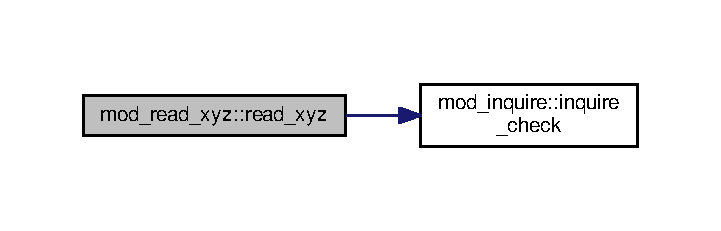
\includegraphics[width=346pt]{namespacemod__read__xyz_aab6d00fb6cfd2cad4e18f8cb69deb456_cgraph}
\end{center}
\end{figure}


\index{mod\+\_\+read\+\_\+xyz@{mod\+\_\+read\+\_\+xyz}!rotate\+\_\+xyz@{rotate\+\_\+xyz}}
\index{rotate\+\_\+xyz@{rotate\+\_\+xyz}!mod\+\_\+read\+\_\+xyz@{mod\+\_\+read\+\_\+xyz}}
\subsubsection[{\texorpdfstring{rotate\+\_\+xyz(this, precession)}{rotate_xyz(this, precession)}}]{\setlength{\rightskip}{0pt plus 5cm}subroutine mod\+\_\+read\+\_\+xyz\+::rotate\+\_\+xyz (
\begin{DoxyParamCaption}
\item[{class( {\bf xyz\+\_\+file} ), intent(inout)}]{this, }
\item[{integer, intent(in)}]{precession}
\end{DoxyParamCaption}
)}\hypertarget{namespacemod__read__xyz_ab1b3f67fa055b9311858ca333970405e}{}\label{namespacemod__read__xyz_ab1b3f67fa055b9311858ca333970405e}


This routine performs rotations of mol2 around mol1. 

\begin{DoxyAuthor}{Author}
Felippe M. Colombari Laboratório de Química Teórica, L\+QT -- U\+F\+S\+Car 
\end{DoxyAuthor}


Definition at line 174 of file mod\+\_\+read\+\_\+xyz.\+f90.



References cosalpha, cosphir, costheta, costhetar, dalpha, mod\+\_\+constants\+::deg2rad, mod\+\_\+input\+\_\+read\+::maxp, mod\+\_\+input\+\_\+read\+::np, sinalpha, sinphir, sintheta, and sinthetar.

\index{mod\+\_\+read\+\_\+xyz@{mod\+\_\+read\+\_\+xyz}!translate\+\_\+xyz@{translate\+\_\+xyz}}
\index{translate\+\_\+xyz@{translate\+\_\+xyz}!mod\+\_\+read\+\_\+xyz@{mod\+\_\+read\+\_\+xyz}}
\subsubsection[{\texorpdfstring{translate\+\_\+xyz(this, reference)}{translate_xyz(this, reference)}}]{\setlength{\rightskip}{0pt plus 5cm}subroutine mod\+\_\+read\+\_\+xyz\+::translate\+\_\+xyz (
\begin{DoxyParamCaption}
\item[{class( {\bf xyz\+\_\+file} ), intent(inout)}]{this, }
\item[{integer, intent(in)}]{reference}
\end{DoxyParamCaption}
)}\hypertarget{namespacemod__read__xyz_a28a0648307ac1a30adc5bf4571709a58}{}\label{namespacemod__read__xyz_a28a0648307ac1a30adc5bf4571709a58}


This routine places \hyperlink{structmod__read__xyz_1_1xyz__file}{xyz\+\_\+file} 1 reference site at origin. 

\begin{DoxyAuthor}{Author}
Felippe M. Colombari Laboratório de Química Teórica, L\+QT -- U\+F\+S\+Car 
\end{DoxyAuthor}


Definition at line 103 of file mod\+\_\+read\+\_\+xyz.\+f90.

\index{mod\+\_\+read\+\_\+xyz@{mod\+\_\+read\+\_\+xyz}!write\+\_\+xyz@{write\+\_\+xyz}}
\index{write\+\_\+xyz@{write\+\_\+xyz}!mod\+\_\+read\+\_\+xyz@{mod\+\_\+read\+\_\+xyz}}
\subsubsection[{\texorpdfstring{write\+\_\+xyz(this, lowest)}{write_xyz(this, lowest)}}]{\setlength{\rightskip}{0pt plus 5cm}subroutine mod\+\_\+read\+\_\+xyz\+::write\+\_\+xyz (
\begin{DoxyParamCaption}
\item[{class( {\bf xyz\+\_\+dimer} ), intent(inout)}]{this, }
\item[{real( kind = dp ), intent(in)}]{lowest}
\end{DoxyParamCaption}
)}\hypertarget{namespacemod__read__xyz_a86235488f0f7fd76cccfa75734903206}{}\label{namespacemod__read__xyz_a86235488f0f7fd76cccfa75734903206}


Definition at line 255 of file mod\+\_\+read\+\_\+xyz.\+f90.



References mol1, and mol2.



\subsection{Variable Documentation}
\index{mod\+\_\+read\+\_\+xyz@{mod\+\_\+read\+\_\+xyz}!cosalpha@{cosalpha}}
\index{cosalpha@{cosalpha}!mod\+\_\+read\+\_\+xyz@{mod\+\_\+read\+\_\+xyz}}
\subsubsection[{\texorpdfstring{cosalpha}{cosalpha}}]{\setlength{\rightskip}{0pt plus 5cm}real( kind = dp ) mod\+\_\+read\+\_\+xyz\+::cosalpha}\hypertarget{namespacemod__read__xyz_a932bb57fc8636b50b040311a48f5f5ff}{}\label{namespacemod__read__xyz_a932bb57fc8636b50b040311a48f5f5ff}


Definition at line 45 of file mod\+\_\+read\+\_\+xyz.\+f90.



Referenced by rotate\+\_\+xyz().

\index{mod\+\_\+read\+\_\+xyz@{mod\+\_\+read\+\_\+xyz}!cosphi@{cosphi}}
\index{cosphi@{cosphi}!mod\+\_\+read\+\_\+xyz@{mod\+\_\+read\+\_\+xyz}}
\subsubsection[{\texorpdfstring{cosphi}{cosphi}}]{\setlength{\rightskip}{0pt plus 5cm}real( kind = dp ) mod\+\_\+read\+\_\+xyz\+::cosphi}\hypertarget{namespacemod__read__xyz_a9ce51beca027f9eeb6aa61284b343add}{}\label{namespacemod__read__xyz_a9ce51beca027f9eeb6aa61284b343add}


Definition at line 45 of file mod\+\_\+read\+\_\+xyz.\+f90.



Referenced by align\+\_\+xyz().

\index{mod\+\_\+read\+\_\+xyz@{mod\+\_\+read\+\_\+xyz}!cosphir@{cosphir}}
\index{cosphir@{cosphir}!mod\+\_\+read\+\_\+xyz@{mod\+\_\+read\+\_\+xyz}}
\subsubsection[{\texorpdfstring{cosphir}{cosphir}}]{\setlength{\rightskip}{0pt plus 5cm}real( kind = dp ) mod\+\_\+read\+\_\+xyz\+::cosphir}\hypertarget{namespacemod__read__xyz_a41be340f1c832ab4905f7e17f6ebe4ff}{}\label{namespacemod__read__xyz_a41be340f1c832ab4905f7e17f6ebe4ff}


Definition at line 46 of file mod\+\_\+read\+\_\+xyz.\+f90.



Referenced by mod\+\_\+loops\+::calc(), rotate\+\_\+xyz(), and mod\+\_\+search\+::search\+\_\+structures().

\index{mod\+\_\+read\+\_\+xyz@{mod\+\_\+read\+\_\+xyz}!costheta@{costheta}}
\index{costheta@{costheta}!mod\+\_\+read\+\_\+xyz@{mod\+\_\+read\+\_\+xyz}}
\subsubsection[{\texorpdfstring{costheta}{costheta}}]{\setlength{\rightskip}{0pt plus 5cm}real( kind = dp ) mod\+\_\+read\+\_\+xyz\+::costheta}\hypertarget{namespacemod__read__xyz_ae522e26e0e7e87987ca7018f36b43903}{}\label{namespacemod__read__xyz_ae522e26e0e7e87987ca7018f36b43903}


Definition at line 45 of file mod\+\_\+read\+\_\+xyz.\+f90.



Referenced by align\+\_\+xyz(), and rotate\+\_\+xyz().

\index{mod\+\_\+read\+\_\+xyz@{mod\+\_\+read\+\_\+xyz}!costhetar@{costhetar}}
\index{costhetar@{costhetar}!mod\+\_\+read\+\_\+xyz@{mod\+\_\+read\+\_\+xyz}}
\subsubsection[{\texorpdfstring{costhetar}{costhetar}}]{\setlength{\rightskip}{0pt plus 5cm}real( kind = dp ) mod\+\_\+read\+\_\+xyz\+::costhetar}\hypertarget{namespacemod__read__xyz_a4fe5cc70aa62a1a36598156d04828c90}{}\label{namespacemod__read__xyz_a4fe5cc70aa62a1a36598156d04828c90}


Definition at line 46 of file mod\+\_\+read\+\_\+xyz.\+f90.



Referenced by mod\+\_\+loops\+::calc(), rotate\+\_\+xyz(), and mod\+\_\+search\+::search\+\_\+structures().

\index{mod\+\_\+read\+\_\+xyz@{mod\+\_\+read\+\_\+xyz}!dalpha@{dalpha}}
\index{dalpha@{dalpha}!mod\+\_\+read\+\_\+xyz@{mod\+\_\+read\+\_\+xyz}}
\subsubsection[{\texorpdfstring{dalpha}{dalpha}}]{\setlength{\rightskip}{0pt plus 5cm}real( kind = dp ) mod\+\_\+read\+\_\+xyz\+::dalpha}\hypertarget{namespacemod__read__xyz_a41a3fdae2ca35a3a22c0ed3bce4ab65f}{}\label{namespacemod__read__xyz_a41a3fdae2ca35a3a22c0ed3bce4ab65f}


Definition at line 44 of file mod\+\_\+read\+\_\+xyz.\+f90.



Referenced by rotate\+\_\+xyz().

\index{mod\+\_\+read\+\_\+xyz@{mod\+\_\+read\+\_\+xyz}!dimers@{dimers}}
\index{dimers@{dimers}!mod\+\_\+read\+\_\+xyz@{mod\+\_\+read\+\_\+xyz}}
\subsubsection[{\texorpdfstring{dimers}{dimers}}]{\setlength{\rightskip}{0pt plus 5cm}type( {\bf xyz\+\_\+dimer} ) mod\+\_\+read\+\_\+xyz\+::dimers}\hypertarget{namespacemod__read__xyz_aa013f111078e556f2e4eee9018cd605a}{}\label{namespacemod__read__xyz_aa013f111078e556f2e4eee9018cd605a}


Definition at line 42 of file mod\+\_\+read\+\_\+xyz.\+f90.



Referenced by mod\+\_\+loops\+::calc(), and mod\+\_\+search\+::search\+\_\+structures().

\index{mod\+\_\+read\+\_\+xyz@{mod\+\_\+read\+\_\+xyz}!dphi@{dphi}}
\index{dphi@{dphi}!mod\+\_\+read\+\_\+xyz@{mod\+\_\+read\+\_\+xyz}}
\subsubsection[{\texorpdfstring{dphi}{dphi}}]{\setlength{\rightskip}{0pt plus 5cm}real( kind = dp ) mod\+\_\+read\+\_\+xyz\+::dphi}\hypertarget{namespacemod__read__xyz_a7d29c731d6db9ccacae5b6e2fb25f4c5}{}\label{namespacemod__read__xyz_a7d29c731d6db9ccacae5b6e2fb25f4c5}


Definition at line 44 of file mod\+\_\+read\+\_\+xyz.\+f90.



Referenced by align\+\_\+xyz().

\index{mod\+\_\+read\+\_\+xyz@{mod\+\_\+read\+\_\+xyz}!dtheta@{dtheta}}
\index{dtheta@{dtheta}!mod\+\_\+read\+\_\+xyz@{mod\+\_\+read\+\_\+xyz}}
\subsubsection[{\texorpdfstring{dtheta}{dtheta}}]{\setlength{\rightskip}{0pt plus 5cm}real( kind = dp ) mod\+\_\+read\+\_\+xyz\+::dtheta}\hypertarget{namespacemod__read__xyz_a12174845302ad3f92b147b671045e952}{}\label{namespacemod__read__xyz_a12174845302ad3f92b147b671045e952}


Definition at line 44 of file mod\+\_\+read\+\_\+xyz.\+f90.



Referenced by align\+\_\+xyz().

\index{mod\+\_\+read\+\_\+xyz@{mod\+\_\+read\+\_\+xyz}!mol1@{mol1}}
\index{mol1@{mol1}!mod\+\_\+read\+\_\+xyz@{mod\+\_\+read\+\_\+xyz}}
\subsubsection[{\texorpdfstring{mol1}{mol1}}]{\setlength{\rightskip}{0pt plus 5cm}type( {\bf xyz\+\_\+file} ) mod\+\_\+read\+\_\+xyz\+::mol1}\hypertarget{namespacemod__read__xyz_a4f9bfbc2e65fbc70f98f0dd5482a86f0}{}\label{namespacemod__read__xyz_a4f9bfbc2e65fbc70f98f0dd5482a86f0}


Definition at line 33 of file mod\+\_\+read\+\_\+xyz.\+f90.



Referenced by build\+\_\+dimer(), mod\+\_\+loops\+::calc(), mod\+\_\+pot\+\_\+ljc\+::calc\+\_\+ljc\+\_\+cross(), mod\+\_\+pot\+\_\+ljc\+::calc\+\_\+ljc\+\_\+energy(), mod\+\_\+read\+\_\+grids\+::center\+\_\+translation\+\_\+grid(), mod\+\_\+pot\+\_\+none\+::check\+\_\+conf(), mod\+\_\+deallocate\+\_\+all\+::deallocate\+\_\+arrays(), mod\+\_\+search\+::search\+\_\+structures(), themis(), and write\+\_\+xyz().

\index{mod\+\_\+read\+\_\+xyz@{mod\+\_\+read\+\_\+xyz}!mol2@{mol2}}
\index{mol2@{mol2}!mod\+\_\+read\+\_\+xyz@{mod\+\_\+read\+\_\+xyz}}
\subsubsection[{\texorpdfstring{mol2}{mol2}}]{\setlength{\rightskip}{0pt plus 5cm}type( {\bf xyz\+\_\+file} ) mod\+\_\+read\+\_\+xyz\+::mol2}\hypertarget{namespacemod__read__xyz_ad6455b07e3bcbb980fd81f7a6a61d835}{}\label{namespacemod__read__xyz_ad6455b07e3bcbb980fd81f7a6a61d835}


Definition at line 33 of file mod\+\_\+read\+\_\+xyz.\+f90.



Referenced by build\+\_\+dimer(), mod\+\_\+loops\+::calc(), mod\+\_\+pot\+\_\+ljc\+::calc\+\_\+ljc\+\_\+cross(), mod\+\_\+pot\+\_\+ljc\+::calc\+\_\+ljc\+\_\+energy(), mod\+\_\+pot\+\_\+none\+::check\+\_\+conf(), mod\+\_\+deallocate\+\_\+all\+::deallocate\+\_\+arrays(), mod\+\_\+search\+::search\+\_\+structures(), themis(), and write\+\_\+xyz().

\index{mod\+\_\+read\+\_\+xyz@{mod\+\_\+read\+\_\+xyz}!sinalpha@{sinalpha}}
\index{sinalpha@{sinalpha}!mod\+\_\+read\+\_\+xyz@{mod\+\_\+read\+\_\+xyz}}
\subsubsection[{\texorpdfstring{sinalpha}{sinalpha}}]{\setlength{\rightskip}{0pt plus 5cm}real( kind = dp ) mod\+\_\+read\+\_\+xyz\+::sinalpha}\hypertarget{namespacemod__read__xyz_a97d484f8583bf1d60e6d02230e28feb3}{}\label{namespacemod__read__xyz_a97d484f8583bf1d60e6d02230e28feb3}


Definition at line 45 of file mod\+\_\+read\+\_\+xyz.\+f90.



Referenced by rotate\+\_\+xyz().

\index{mod\+\_\+read\+\_\+xyz@{mod\+\_\+read\+\_\+xyz}!sinphi@{sinphi}}
\index{sinphi@{sinphi}!mod\+\_\+read\+\_\+xyz@{mod\+\_\+read\+\_\+xyz}}
\subsubsection[{\texorpdfstring{sinphi}{sinphi}}]{\setlength{\rightskip}{0pt plus 5cm}real( kind = dp ) mod\+\_\+read\+\_\+xyz\+::sinphi}\hypertarget{namespacemod__read__xyz_a183d28b4e8d41fd8eefe9239450cb5f7}{}\label{namespacemod__read__xyz_a183d28b4e8d41fd8eefe9239450cb5f7}


Definition at line 45 of file mod\+\_\+read\+\_\+xyz.\+f90.



Referenced by align\+\_\+xyz().

\index{mod\+\_\+read\+\_\+xyz@{mod\+\_\+read\+\_\+xyz}!sinphir@{sinphir}}
\index{sinphir@{sinphir}!mod\+\_\+read\+\_\+xyz@{mod\+\_\+read\+\_\+xyz}}
\subsubsection[{\texorpdfstring{sinphir}{sinphir}}]{\setlength{\rightskip}{0pt plus 5cm}real( kind = dp ) mod\+\_\+read\+\_\+xyz\+::sinphir}\hypertarget{namespacemod__read__xyz_a446fc19de6fe61df592b2f68c8a86ca3}{}\label{namespacemod__read__xyz_a446fc19de6fe61df592b2f68c8a86ca3}


Definition at line 46 of file mod\+\_\+read\+\_\+xyz.\+f90.



Referenced by mod\+\_\+loops\+::calc(), rotate\+\_\+xyz(), and mod\+\_\+search\+::search\+\_\+structures().

\index{mod\+\_\+read\+\_\+xyz@{mod\+\_\+read\+\_\+xyz}!sintheta@{sintheta}}
\index{sintheta@{sintheta}!mod\+\_\+read\+\_\+xyz@{mod\+\_\+read\+\_\+xyz}}
\subsubsection[{\texorpdfstring{sintheta}{sintheta}}]{\setlength{\rightskip}{0pt plus 5cm}real( kind = dp ) mod\+\_\+read\+\_\+xyz\+::sintheta}\hypertarget{namespacemod__read__xyz_af660cbed16517234379cfffe0132378f}{}\label{namespacemod__read__xyz_af660cbed16517234379cfffe0132378f}


Definition at line 45 of file mod\+\_\+read\+\_\+xyz.\+f90.



Referenced by align\+\_\+xyz(), and rotate\+\_\+xyz().

\index{mod\+\_\+read\+\_\+xyz@{mod\+\_\+read\+\_\+xyz}!sinthetar@{sinthetar}}
\index{sinthetar@{sinthetar}!mod\+\_\+read\+\_\+xyz@{mod\+\_\+read\+\_\+xyz}}
\subsubsection[{\texorpdfstring{sinthetar}{sinthetar}}]{\setlength{\rightskip}{0pt plus 5cm}real( kind = dp ) mod\+\_\+read\+\_\+xyz\+::sinthetar}\hypertarget{namespacemod__read__xyz_ad3f08d13679d5f31c776b74f1abe0da5}{}\label{namespacemod__read__xyz_ad3f08d13679d5f31c776b74f1abe0da5}


Definition at line 46 of file mod\+\_\+read\+\_\+xyz.\+f90.



Referenced by mod\+\_\+loops\+::calc(), rotate\+\_\+xyz(), and mod\+\_\+search\+::search\+\_\+structures().


\hypertarget{namespacemod__resume}{}\section{mod\+\_\+resume Module Reference}
\label{namespacemod__resume}\index{mod\+\_\+resume@{mod\+\_\+resume}}


This module contains routines that resume the run.  


\subsection*{Functions/\+Subroutines}
\begin{DoxyCompactItemize}
\item 
subroutine \hyperlink{namespacemod__resume_a74e0ed44fafff381d91477160c6d8a74}{ending} (timet)
\begin{DoxyCompactList}\small\item\em This routine writes details of the calculation on screen. \end{DoxyCompactList}\item 
subroutine \hyperlink{namespacemod__resume_a36133bfde88e19b38e5d5245c89843fe}{sort\+\_\+output}
\begin{DoxyCompactList}\small\item\em This routine sorts central grid points according to their free energy values. \end{DoxyCompactList}\end{DoxyCompactItemize}
\subsection*{Variables}
\begin{DoxyCompactItemize}
\item 
real(kind=dp), dimension(\+:), allocatable \hyperlink{namespacemod__resume_ad3cf0f0162ccc00d0efebb0348fe6ae5}{a\+\_\+min}
\item 
integer, dimension(1) \hyperlink{namespacemod__resume_a2861e2f353be05850b4ad384446859c6}{pos\+\_\+a\+\_\+min}
\end{DoxyCompactItemize}


\subsection{Detailed Description}
This module contains routines that resume the run. 

\begin{DoxyAuthor}{Author}
Felippe M. Colombari
\begin{DoxyItemize}
\item Laboratório de Química Teórica, L\+QT -- U\+F\+S\+Car 
\end{DoxyItemize}
\end{DoxyAuthor}
\begin{DoxyDate}{Date}
-\/ Jun, 2017
\begin{DoxyItemize}
\item independent module created 
\end{DoxyItemize}
\end{DoxyDate}


\subsection{Function/\+Subroutine Documentation}
\mbox{\Hypertarget{namespacemod__resume_a74e0ed44fafff381d91477160c6d8a74}\label{namespacemod__resume_a74e0ed44fafff381d91477160c6d8a74}} 
\index{mod\+\_\+resume@{mod\+\_\+resume}!ending@{ending}}
\index{ending@{ending}!mod\+\_\+resume@{mod\+\_\+resume}}
\subsubsection{\texorpdfstring{ending()}{ending()}}
{\footnotesize\ttfamily subroutine mod\+\_\+resume\+::ending (\begin{DoxyParamCaption}\item[{real( kind = dp ), intent(in)}]{timet }\end{DoxyParamCaption})}



This routine writes details of the calculation on screen. 

\begin{DoxyAuthor}{Author}
Felippe M. Colombari
\begin{DoxyItemize}
\item Laboratório de Química Teórica, L\+QT -- U\+F\+S\+Car 
\end{DoxyItemize}
\end{DoxyAuthor}
\begin{DoxyDate}{Date}
-\/ Jun, 2017
\begin{DoxyItemize}
\item subroutine created 
\end{DoxyItemize}
\end{DoxyDate}


Definition at line 33 of file mod\+\_\+resume.\+f90.



References mod\+\_\+read\+\_\+grids\+::a, mod\+\_\+input\+\_\+read\+::atom\+\_\+overlap, mod\+\_\+constants\+::dashline, mod\+\_\+cmd\+\_\+line\+::grid\+\_\+type, mod\+\_\+cmd\+\_\+line\+::irun, mod\+\_\+loops\+::min\+\_\+ener, mod\+\_\+search\+::n, mod\+\_\+input\+\_\+read\+::potential, and mod\+\_\+cmd\+\_\+line\+::rad.



Referenced by themis().

\mbox{\Hypertarget{namespacemod__resume_a36133bfde88e19b38e5d5245c89843fe}\label{namespacemod__resume_a36133bfde88e19b38e5d5245c89843fe}} 
\index{mod\+\_\+resume@{mod\+\_\+resume}!sort\+\_\+output@{sort\+\_\+output}}
\index{sort\+\_\+output@{sort\+\_\+output}!mod\+\_\+resume@{mod\+\_\+resume}}
\subsubsection{\texorpdfstring{sort\+\_\+output()}{sort\_output()}}
{\footnotesize\ttfamily subroutine mod\+\_\+resume\+::sort\+\_\+output (\begin{DoxyParamCaption}{ }\end{DoxyParamCaption})}



This routine sorts central grid points according to their free energy values. 

\begin{DoxyAuthor}{Author}
Felippe M. Colombari
\begin{DoxyItemize}
\item Laboratório de Química Teórica, L\+QT -- U\+F\+S\+Car 
\end{DoxyItemize}
\end{DoxyAuthor}
\begin{DoxyDate}{Date}
-\/ Aug, 2017
\begin{DoxyItemize}
\item subroutine created 
\end{DoxyItemize}
\end{DoxyDate}
\begin{DoxyNote}{Note}
~\newline

\begin{DoxyItemize}
\item The method used to sort the free energy array is non-\/standard, but is much more easier to implement and faster to run\+: ~\newline
 i) The lowest free energy value is found on array A and saved at first position of array B; ii) In array A, such position is replaced by I\+N\+F\+I\+N\+I\+TY; ~\newline
 iii) Now the lowest free energy value from array A will be the second value from array B and so on... 
\end{DoxyItemize}
\end{DoxyNote}


Definition at line 106 of file mod\+\_\+resume.\+f90.



References mod\+\_\+read\+\_\+grids\+::a, a\+\_\+min, mod\+\_\+loops\+::atotal, mod\+\_\+constants\+::dashline, mod\+\_\+read\+\_\+grids\+::eavg, mod\+\_\+loops\+::etotalavg, mod\+\_\+constants\+::fpinf, mod\+\_\+read\+\_\+grids\+::grid\+\_\+trans, mod\+\_\+loops\+::kbt, mod\+\_\+loops\+::min\+\_\+ener, mod\+\_\+read\+\_\+grids\+::mts, mod\+\_\+loops\+::mtstotal, pos\+\_\+a\+\_\+min, mod\+\_\+read\+\_\+grids\+::probt, and mod\+\_\+loops\+::ztrans.



Referenced by themis().



\subsection{Variable Documentation}
\mbox{\Hypertarget{namespacemod__resume_ad3cf0f0162ccc00d0efebb0348fe6ae5}\label{namespacemod__resume_ad3cf0f0162ccc00d0efebb0348fe6ae5}} 
\index{mod\+\_\+resume@{mod\+\_\+resume}!a\+\_\+min@{a\+\_\+min}}
\index{a\+\_\+min@{a\+\_\+min}!mod\+\_\+resume@{mod\+\_\+resume}}
\subsubsection{\texorpdfstring{a\+\_\+min}{a\_min}}
{\footnotesize\ttfamily real( kind = dp ), dimension(\+:), allocatable mod\+\_\+resume\+::a\+\_\+min}



Definition at line 19 of file mod\+\_\+resume.\+f90.



Referenced by sort\+\_\+output().

\mbox{\Hypertarget{namespacemod__resume_a2861e2f353be05850b4ad384446859c6}\label{namespacemod__resume_a2861e2f353be05850b4ad384446859c6}} 
\index{mod\+\_\+resume@{mod\+\_\+resume}!pos\+\_\+a\+\_\+min@{pos\+\_\+a\+\_\+min}}
\index{pos\+\_\+a\+\_\+min@{pos\+\_\+a\+\_\+min}!mod\+\_\+resume@{mod\+\_\+resume}}
\subsubsection{\texorpdfstring{pos\+\_\+a\+\_\+min}{pos\_a\_min}}
{\footnotesize\ttfamily integer, dimension(1) mod\+\_\+resume\+::pos\+\_\+a\+\_\+min}



Definition at line 20 of file mod\+\_\+resume.\+f90.



Referenced by sort\+\_\+output().


\hypertarget{namespacemod__search}{}\section{mod\+\_\+search Module Reference}
\label{namespacemod__search}\index{mod\+\_\+search@{mod\+\_\+search}}


This module contains routines to search and write the lowest energy structures for the run.  


\subsection*{Functions/\+Subroutines}
\begin{DoxyCompactItemize}
\item 
subroutine \hyperlink{namespacemod__search_a5026804a4e265b1a450eebc86cd81575}{count\+\_\+structures}
\begin{DoxyCompactList}\small\item\em This routine counts the number of structures with energy closer (within 0.\+5 $\ast$ k\+BT) to the most stable one. \end{DoxyCompactList}\item 
subroutine \hyperlink{namespacemod__search_a55e1f850472fe6cef190a6838ae61e51}{sort\+\_\+energy}
\begin{DoxyCompactList}\small\item\em This routine sorts the energy array and write its first n values to energy-\/sort.\+log. \end{DoxyCompactList}\item 
subroutine \hyperlink{namespacemod__search_ac11978e9ebdb6b101a09555f4742a4c9}{search\+\_\+structures}
\begin{DoxyCompactList}\small\item\em This routine generates the configurations for structures written at energy-\/sort.\+log. \end{DoxyCompactList}\end{DoxyCompactItemize}
\subsection*{Variables}
\begin{DoxyCompactItemize}
\item 
real(kind=dp) \hyperlink{namespacemod__search_a014567a8f5474b311cedf2f9b1dbda1a}{lowest}
\item 
integer, dimension(3) \hyperlink{namespacemod__search_a018a3c64ea9e25b0dfc15ebe763920cf}{pos\+\_\+min\+\_\+energy}
\item 
integer \hyperlink{namespacemod__search_a0c7388c12d8e6a95b8c3f9fd86321687}{n}
\item 
real(kind=dp), dimension(\+:), allocatable \hyperlink{namespacemod__search_a8ce72764a5658f7958ed5c473dd77706}{energy\+\_\+ordered}
\end{DoxyCompactItemize}


\subsection{Detailed Description}
This module contains routines to search and write the lowest energy structures for the run. 

\begin{DoxyAuthor}{Author}
Felippe M. Colombari
\begin{DoxyItemize}
\item Laboratório de Química Teórica, L\+QT -- U\+F\+S\+Car 
\end{DoxyItemize}
\end{DoxyAuthor}
\begin{DoxyDate}{Date}
-\/ Sep, 2017
\begin{DoxyItemize}
\item independent module created 
\end{DoxyItemize}

-\/ Jan, 2018
\begin{DoxyItemize}
\item documentation and support added 
\end{DoxyItemize}
\end{DoxyDate}


\subsection{Function/\+Subroutine Documentation}
\index{mod\+\_\+search@{mod\+\_\+search}!count\+\_\+structures@{count\+\_\+structures}}
\index{count\+\_\+structures@{count\+\_\+structures}!mod\+\_\+search@{mod\+\_\+search}}
\subsubsection[{\texorpdfstring{count\+\_\+structures}{count_structures}}]{\setlength{\rightskip}{0pt plus 5cm}subroutine mod\+\_\+search\+::count\+\_\+structures (
\begin{DoxyParamCaption}
{}
\end{DoxyParamCaption}
)}\hypertarget{namespacemod__search_a5026804a4e265b1a450eebc86cd81575}{}\label{namespacemod__search_a5026804a4e265b1a450eebc86cd81575}


This routine counts the number of structures with energy closer (within 0.\+5 $\ast$ k\+BT) to the most stable one. 

\begin{DoxyAuthor}{Author}
Felippe M. Colombari Laboratório de Química Teórica, L\+QT -- U\+F\+S\+Car 
\end{DoxyAuthor}


Definition at line 36 of file mod\+\_\+search.\+f90.



References mod\+\_\+read\+\_\+grids\+::grid\+\_\+rot, mod\+\_\+read\+\_\+grids\+::grid\+\_\+trans, mod\+\_\+loops\+::kbt, mod\+\_\+loops\+::min\+\_\+ener, n, mod\+\_\+input\+\_\+read\+::np, and mod\+\_\+read\+\_\+grids\+::vtot.



Referenced by themis().

\index{mod\+\_\+search@{mod\+\_\+search}!search\+\_\+structures@{search\+\_\+structures}}
\index{search\+\_\+structures@{search\+\_\+structures}!mod\+\_\+search@{mod\+\_\+search}}
\subsubsection[{\texorpdfstring{search\+\_\+structures}{search_structures}}]{\setlength{\rightskip}{0pt plus 5cm}subroutine mod\+\_\+search\+::search\+\_\+structures (
\begin{DoxyParamCaption}
{}
\end{DoxyParamCaption}
)}\hypertarget{namespacemod__search_ac11978e9ebdb6b101a09555f4742a4c9}{}\label{namespacemod__search_ac11978e9ebdb6b101a09555f4742a4c9}


This routine generates the configurations for structures written at energy-\/sort.\+log. 

\begin{DoxyAuthor}{Author}
Felippe M. Colombari
\begin{DoxyItemize}
\item Laboratório de Química Teórica, L\+QT -- U\+F\+S\+Car 
\end{DoxyItemize}
\end{DoxyAuthor}
\begin{DoxyDate}{Date}
-\/ Sep, 2017
\begin{DoxyItemize}
\item subroutine created 
\end{DoxyItemize}
\end{DoxyDate}


Definition at line 146 of file mod\+\_\+search.\+f90.



References mod\+\_\+read\+\_\+xyz\+::cosphir, mod\+\_\+read\+\_\+xyz\+::costhetar, mod\+\_\+read\+\_\+xyz\+::dimers, energy\+\_\+ordered, mod\+\_\+read\+\_\+grids\+::grid\+\_\+rot, mod\+\_\+read\+\_\+grids\+::grid\+\_\+trans, mod\+\_\+inquire\+::inquire\+\_\+check(), lowest, mod\+\_\+read\+\_\+xyz\+::mol1, mod\+\_\+read\+\_\+xyz\+::mol2, mod\+\_\+input\+\_\+read\+::nstruc, mod\+\_\+read\+\_\+grids\+::phir, mod\+\_\+input\+\_\+read\+::ref1, mod\+\_\+input\+\_\+read\+::ref2, mod\+\_\+read\+\_\+xyz\+::sinphir, mod\+\_\+read\+\_\+xyz\+::sinthetar, mod\+\_\+read\+\_\+grids\+::thetar, mod\+\_\+input\+\_\+read\+::vector1, and mod\+\_\+input\+\_\+read\+::vector2.



Referenced by themis().



Here is the call graph for this function\+:\nopagebreak
\begin{figure}[H]
\begin{center}
\leavevmode
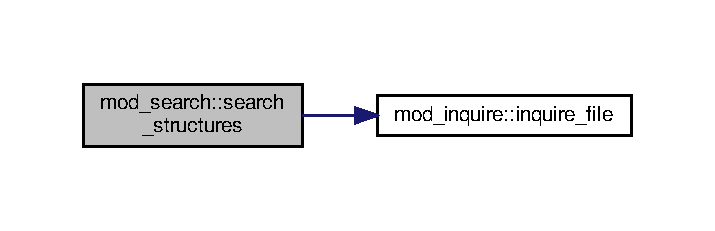
\includegraphics[width=325pt]{namespacemod__search_ac11978e9ebdb6b101a09555f4742a4c9_cgraph}
\end{center}
\end{figure}


\index{mod\+\_\+search@{mod\+\_\+search}!sort\+\_\+energy@{sort\+\_\+energy}}
\index{sort\+\_\+energy@{sort\+\_\+energy}!mod\+\_\+search@{mod\+\_\+search}}
\subsubsection[{\texorpdfstring{sort\+\_\+energy}{sort_energy}}]{\setlength{\rightskip}{0pt plus 5cm}subroutine mod\+\_\+search\+::sort\+\_\+energy (
\begin{DoxyParamCaption}
{}
\end{DoxyParamCaption}
)}\hypertarget{namespacemod__search_a55e1f850472fe6cef190a6838ae61e51}{}\label{namespacemod__search_a55e1f850472fe6cef190a6838ae61e51}


This routine sorts the energy array and write its first n values to energy-\/sort.\+log. 

\begin{DoxyAuthor}{Author}
Felippe M. Colombari
\begin{DoxyItemize}
\item Laboratório de Química Teórica, L\+QT -- U\+F\+S\+Car 
\end{DoxyItemize}
\end{DoxyAuthor}
\begin{DoxyDate}{Date}
-\/ Sep, 2017
\begin{DoxyItemize}
\item subroutine created 
\end{DoxyItemize}
\end{DoxyDate}
\begin{DoxyNote}{Note}
~\newline

\begin{DoxyItemize}
\item The method used to sort the energy array is non-\/standard, but is much more easier to implement and faster to run\+: ~\newline
 i) The lowest energy value is found on array A and saved at first position of array B; ii) In array A, such position is replaced by I\+N\+F\+I\+N\+I\+TY; ~\newline
 iii) Now the lowest energy value from array A will be the second value from array B and so on... 
\end{DoxyItemize}
\end{DoxyNote}


Definition at line 87 of file mod\+\_\+search.\+f90.



References energy\+\_\+ordered, mod\+\_\+constants\+::fpinf, mod\+\_\+loops\+::kbt, mod\+\_\+loops\+::min\+\_\+ener, mod\+\_\+input\+\_\+read\+::nstruc, pos\+\_\+min\+\_\+energy, mod\+\_\+read\+\_\+grids\+::vtot, and mod\+\_\+loops\+::ztrans.



Referenced by themis().



\subsection{Variable Documentation}
\index{mod\+\_\+search@{mod\+\_\+search}!energy\+\_\+ordered@{energy\+\_\+ordered}}
\index{energy\+\_\+ordered@{energy\+\_\+ordered}!mod\+\_\+search@{mod\+\_\+search}}
\subsubsection[{\texorpdfstring{energy\+\_\+ordered}{energy_ordered}}]{\setlength{\rightskip}{0pt plus 5cm}real( kind = dp ), dimension(\+:), allocatable mod\+\_\+search\+::energy\+\_\+ordered}\hypertarget{namespacemod__search_a8ce72764a5658f7958ed5c473dd77706}{}\label{namespacemod__search_a8ce72764a5658f7958ed5c473dd77706}


Definition at line 24 of file mod\+\_\+search.\+f90.



Referenced by search\+\_\+structures(), and sort\+\_\+energy().

\index{mod\+\_\+search@{mod\+\_\+search}!lowest@{lowest}}
\index{lowest@{lowest}!mod\+\_\+search@{mod\+\_\+search}}
\subsubsection[{\texorpdfstring{lowest}{lowest}}]{\setlength{\rightskip}{0pt plus 5cm}real( kind = dp ) mod\+\_\+search\+::lowest}\hypertarget{namespacemod__search_a014567a8f5474b311cedf2f9b1dbda1a}{}\label{namespacemod__search_a014567a8f5474b311cedf2f9b1dbda1a}


Definition at line 22 of file mod\+\_\+search.\+f90.



Referenced by search\+\_\+structures().

\index{mod\+\_\+search@{mod\+\_\+search}!n@{n}}
\index{n@{n}!mod\+\_\+search@{mod\+\_\+search}}
\subsubsection[{\texorpdfstring{n}{n}}]{\setlength{\rightskip}{0pt plus 5cm}integer mod\+\_\+search\+::n}\hypertarget{namespacemod__search_a0c7388c12d8e6a95b8c3f9fd86321687}{}\label{namespacemod__search_a0c7388c12d8e6a95b8c3f9fd86321687}


Definition at line 23 of file mod\+\_\+search.\+f90.



Referenced by count\+\_\+structures(), and mod\+\_\+resume\+::ending().

\index{mod\+\_\+search@{mod\+\_\+search}!pos\+\_\+min\+\_\+energy@{pos\+\_\+min\+\_\+energy}}
\index{pos\+\_\+min\+\_\+energy@{pos\+\_\+min\+\_\+energy}!mod\+\_\+search@{mod\+\_\+search}}
\subsubsection[{\texorpdfstring{pos\+\_\+min\+\_\+energy}{pos_min_energy}}]{\setlength{\rightskip}{0pt plus 5cm}integer, dimension(3) mod\+\_\+search\+::pos\+\_\+min\+\_\+energy}\hypertarget{namespacemod__search_a018a3c64ea9e25b0dfc15ebe763920cf}{}\label{namespacemod__search_a018a3c64ea9e25b0dfc15ebe763920cf}


Definition at line 23 of file mod\+\_\+search.\+f90.



Referenced by sort\+\_\+energy().


\hypertarget{namespacemod__spherical__grids}{}\section{mod\+\_\+spherical\+\_\+grids Module Reference}
\label{namespacemod__spherical__grids}\index{mod\+\_\+spherical\+\_\+grids@{mod\+\_\+spherical\+\_\+grids}}
\subsection*{Functions/\+Subroutines}
\begin{DoxyCompactItemize}
\item 
subroutine \hyperlink{namespacemod__spherical__grids_ac770a39945e60a262069f9f186819614}{icos\+\_\+shape} (point\+\_\+num, edge\+\_\+num, face\+\_\+num, face\+\_\+order\+\_\+max, point\+\_\+coord, edge\+\_\+point, face\+\_\+order, face\+\_\+point)
\item 
subroutine \hyperlink{namespacemod__spherical__grids_a98d8c41d6d666f6c3fe1dbadcf0dba89}{icos\+\_\+num} (point\+\_\+num, edge\+\_\+num, face\+\_\+num, face\+\_\+order\+\_\+max)
\item 
real(kind=dp) function \hyperlink{namespacemod__spherical__grids_adbe3eff686f6254a50a5afd75255c2c8}{r8vec\+\_\+norm} (n, a)
\item 
subroutine \hyperlink{namespacemod__spherical__grids_a58af853045eb54cbf3a8515e0f48b23b}{sphere\+\_\+icos1\+\_\+points} (factor, node\+\_\+num, node\+\_\+xyz)
\end{DoxyCompactItemize}


\subsection{Detailed Description}
\begin{DoxyNote}{Note}
added error handling 
\end{DoxyNote}
\begin{DoxyDate}{Date}
-\/ Nov 2019 
\end{DoxyDate}


\subsection{Function/\+Subroutine Documentation}
\mbox{\Hypertarget{namespacemod__spherical__grids_a98d8c41d6d666f6c3fe1dbadcf0dba89}\label{namespacemod__spherical__grids_a98d8c41d6d666f6c3fe1dbadcf0dba89}} 
\index{mod\+\_\+spherical\+\_\+grids@{mod\+\_\+spherical\+\_\+grids}!icos\+\_\+num@{icos\+\_\+num}}
\index{icos\+\_\+num@{icos\+\_\+num}!mod\+\_\+spherical\+\_\+grids@{mod\+\_\+spherical\+\_\+grids}}
\subsubsection{\texorpdfstring{icos\+\_\+num()}{icos\_num()}}
{\footnotesize\ttfamily subroutine mod\+\_\+spherical\+\_\+grids\+::icos\+\_\+num (\begin{DoxyParamCaption}\item[{integer(kind=4)}]{point\+\_\+num,  }\item[{integer(kind=4)}]{edge\+\_\+num,  }\item[{integer(kind=4)}]{face\+\_\+num,  }\item[{integer(kind=4)}]{face\+\_\+order\+\_\+max }\end{DoxyParamCaption})}



Definition at line 181 of file mod\+\_\+spherical\+\_\+grids.\+f90.



Referenced by sphere\+\_\+icos1\+\_\+points().

\mbox{\Hypertarget{namespacemod__spherical__grids_ac770a39945e60a262069f9f186819614}\label{namespacemod__spherical__grids_ac770a39945e60a262069f9f186819614}} 
\index{mod\+\_\+spherical\+\_\+grids@{mod\+\_\+spherical\+\_\+grids}!icos\+\_\+shape@{icos\+\_\+shape}}
\index{icos\+\_\+shape@{icos\+\_\+shape}!mod\+\_\+spherical\+\_\+grids@{mod\+\_\+spherical\+\_\+grids}}
\subsubsection{\texorpdfstring{icos\+\_\+shape()}{icos\_shape()}}
{\footnotesize\ttfamily subroutine mod\+\_\+spherical\+\_\+grids\+::icos\+\_\+shape (\begin{DoxyParamCaption}\item[{integer(kind=4)}]{point\+\_\+num,  }\item[{integer(kind=4)}]{edge\+\_\+num,  }\item[{integer(kind=4)}]{face\+\_\+num,  }\item[{integer(kind=4)}]{face\+\_\+order\+\_\+max,  }\item[{real(kind=dp), dimension(3,point\+\_\+num)}]{point\+\_\+coord,  }\item[{integer(kind=4), dimension(edge\+\_\+order,edge\+\_\+num)}]{edge\+\_\+point,  }\item[{integer(kind=4), dimension(face\+\_\+num)}]{face\+\_\+order,  }\item[{integer(kind=4), dimension(face\+\_\+order\+\_\+max,face\+\_\+num)}]{face\+\_\+point }\end{DoxyParamCaption})}



Definition at line 14 of file mod\+\_\+spherical\+\_\+grids.\+f90.



Referenced by sphere\+\_\+icos1\+\_\+points().

\mbox{\Hypertarget{namespacemod__spherical__grids_adbe3eff686f6254a50a5afd75255c2c8}\label{namespacemod__spherical__grids_adbe3eff686f6254a50a5afd75255c2c8}} 
\index{mod\+\_\+spherical\+\_\+grids@{mod\+\_\+spherical\+\_\+grids}!r8vec\+\_\+norm@{r8vec\+\_\+norm}}
\index{r8vec\+\_\+norm@{r8vec\+\_\+norm}!mod\+\_\+spherical\+\_\+grids@{mod\+\_\+spherical\+\_\+grids}}
\subsubsection{\texorpdfstring{r8vec\+\_\+norm()}{r8vec\_norm()}}
{\footnotesize\ttfamily real(kind=dp) function mod\+\_\+spherical\+\_\+grids\+::r8vec\+\_\+norm (\begin{DoxyParamCaption}\item[{integer(kind=4)}]{n,  }\item[{real(kind=dp), dimension(n)}]{a }\end{DoxyParamCaption})}



Definition at line 226 of file mod\+\_\+spherical\+\_\+grids.\+f90.



Referenced by sphere\+\_\+icos1\+\_\+points().

\mbox{\Hypertarget{namespacemod__spherical__grids_a58af853045eb54cbf3a8515e0f48b23b}\label{namespacemod__spherical__grids_a58af853045eb54cbf3a8515e0f48b23b}} 
\index{mod\+\_\+spherical\+\_\+grids@{mod\+\_\+spherical\+\_\+grids}!sphere\+\_\+icos1\+\_\+points@{sphere\+\_\+icos1\+\_\+points}}
\index{sphere\+\_\+icos1\+\_\+points@{sphere\+\_\+icos1\+\_\+points}!mod\+\_\+spherical\+\_\+grids@{mod\+\_\+spherical\+\_\+grids}}
\subsubsection{\texorpdfstring{sphere\+\_\+icos1\+\_\+points()}{sphere\_icos1\_points()}}
{\footnotesize\ttfamily subroutine mod\+\_\+spherical\+\_\+grids\+::sphere\+\_\+icos1\+\_\+points (\begin{DoxyParamCaption}\item[{integer(kind=4)}]{factor,  }\item[{integer(kind=4)}]{node\+\_\+num,  }\item[{real(kind=dp), dimension(3,node\+\_\+num)}]{node\+\_\+xyz }\end{DoxyParamCaption})}



Definition at line 274 of file mod\+\_\+spherical\+\_\+grids.\+f90.



References icos\+\_\+num(), icos\+\_\+shape(), and r8vec\+\_\+norm().



Referenced by mod\+\_\+read\+\_\+grids\+::build\+\_\+reorientation\+\_\+sphere(), and mod\+\_\+read\+\_\+grids\+::build\+\_\+translation\+\_\+sphere().

Here is the call graph for this function\+:
\nopagebreak
\begin{figure}[H]
\begin{center}
\leavevmode
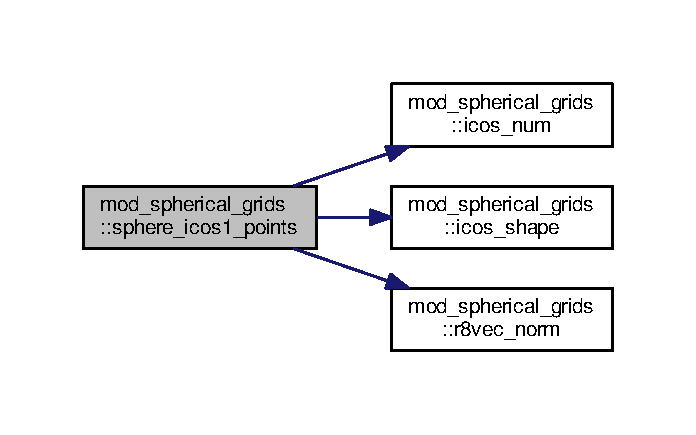
\includegraphics[width=334pt]{namespacemod__spherical__grids_a58af853045eb54cbf3a8515e0f48b23b_cgraph}
\end{center}
\end{figure}

\hypertarget{namespacemod__vmd}{}\section{mod\+\_\+vmd Module Reference}
\label{namespacemod__vmd}\index{mod\+\_\+vmd@{mod\+\_\+vmd}}


This module contains instructions to write V\+MD scripts for visualization of properties around central grid.  


\subsection*{Functions/\+Subroutines}
\begin{DoxyCompactItemize}
\item 
subroutine \hyperlink{namespacemod__vmd_a22ecc122e04e73317480e5b7d6ba38ce}{write\+\_\+vmd\+\_\+files}
\begin{DoxyCompactList}\small\item\em This routine generates .vmd script files to visualize A, E and -\/\+TS along central grid. \end{DoxyCompactList}\end{DoxyCompactItemize}


\subsection{Detailed Description}
This module contains instructions to write V\+MD scripts for visualization of properties around central grid. 

\begin{DoxyAuthor}{Author}
Felippe M. Colombari
\begin{DoxyItemize}
\item Laboratório de Química Teórica, L\+QT -- U\+F\+S\+Car 
\end{DoxyItemize}
\end{DoxyAuthor}
\begin{DoxyDate}{Date}
-\/ Oct, 2017
\begin{DoxyItemize}
\item module created 
\end{DoxyItemize}
\end{DoxyDate}


\subsection{Function/\+Subroutine Documentation}
\index{mod\+\_\+vmd@{mod\+\_\+vmd}!write\+\_\+vmd\+\_\+files@{write\+\_\+vmd\+\_\+files}}
\index{write\+\_\+vmd\+\_\+files@{write\+\_\+vmd\+\_\+files}!mod\+\_\+vmd@{mod\+\_\+vmd}}
\subsubsection[{\texorpdfstring{write\+\_\+vmd\+\_\+files}{write_vmd_files}}]{\setlength{\rightskip}{0pt plus 5cm}subroutine mod\+\_\+vmd\+::write\+\_\+vmd\+\_\+files (
\begin{DoxyParamCaption}
{}
\end{DoxyParamCaption}
)}\hypertarget{namespacemod__vmd_a22ecc122e04e73317480e5b7d6ba38ce}{}\label{namespacemod__vmd_a22ecc122e04e73317480e5b7d6ba38ce}


This routine generates .vmd script files to visualize A, E and -\/\+TS along central grid. 

\begin{DoxyAuthor}{Author}
Felippe M. Colombari
\begin{DoxyItemize}
\item Laboratório de Química Teórica, L\+QT -- U\+F\+S\+Car 
\end{DoxyItemize}
\end{DoxyAuthor}
\begin{DoxyDate}{Date}
-\/ Jun, 2017
\begin{DoxyItemize}
\item subroutine created 
\end{DoxyItemize}

-\/ Dec, 2018
\begin{DoxyItemize}
\item no P\+DB files needed.... / 
\end{DoxyItemize}
\end{DoxyDate}


Definition at line 31 of file mod\+\_\+vmd.\+f90.



References mod\+\_\+read\+\_\+grids\+::a, mod\+\_\+constants\+::dp, mod\+\_\+read\+\_\+grids\+::eavg, and mod\+\_\+read\+\_\+grids\+::mts.



Referenced by themis().


\hypertarget{namespacexdr}{}\section{xdr Module Reference}
\label{namespacexdr}\index{xdr@{xdr}}


X\+DR Fortran Interface with Wrappers.  


\subsection*{Data Types}
\begin{DoxyCompactItemize}
\item 
type \hyperlink{structxdr_1_1xtcfile}{xtcfile}
\end{DoxyCompactItemize}


\subsection{Detailed Description}
X\+DR Fortran Interface with Wrappers. 

\begin{DoxyAuthor}{Author}
James W. Barnett \href{mailto:jbarnet4@tulane.edu}{\tt jbarnet4@tulane.\+edu} \href{https://github.com/wesbarnett/}{\tt https\+://github.\+com/wesbarnett/} 
\end{DoxyAuthor}
\begin{DoxyNote}{Note}
Modified by Kai-\/\+Min Tu (2014) Based on Barnett\textquotesingle{}s work, the interface for T\+RR file is incorporated \href{https://github.com/kmtu/}{\tt https\+://github.\+com/kmtu/} 
\end{DoxyNote}
\begin{DoxyDate}{Date}
2014 
\end{DoxyDate}

\chapter{Class Documentation}
\hypertarget{structmod__pot__ljc_1_1dimer__ljc}{}\section{mod\+\_\+pot\+\_\+ljc\+:\+:dimer\+\_\+ljc Type Reference}
\label{structmod__pot__ljc_1_1dimer__ljc}\index{mod\+\_\+pot\+\_\+ljc\+::dimer\+\_\+ljc@{mod\+\_\+pot\+\_\+ljc\+::dimer\+\_\+ljc}}
\subsection*{Public Member Functions}
\begin{DoxyCompactItemize}
\item 
procedure \hyperlink{structmod__pot__ljc_1_1dimer__ljc_a72bbaa1bb85f42ccaf1907a3b7078d6e}{calc\+\_\+ljc\+\_\+cross}
\item 
procedure \hyperlink{structmod__pot__ljc_1_1dimer__ljc_a38cbfad004776de1ca29fa902aa5e26b}{calc\+\_\+ljc\+\_\+energy}
\end{DoxyCompactItemize}
\subsection*{Public Attributes}
\begin{DoxyCompactItemize}
\item 
real(kind=dp) \hyperlink{structmod__pot__ljc_1_1dimer__ljc_aebc58106f2ca84012cc909153736ade3}{pot\+\_\+lj}
\item 
real(kind=dp) \hyperlink{structmod__pot__ljc_1_1dimer__ljc_ae8cfe31b601f19d7fec86f87c79669b1}{pot\+\_\+coul}
\item 
real(kind=dp), dimension(\+:,\+:), allocatable \hyperlink{structmod__pot__ljc_1_1dimer__ljc_a0b8a2e1fcfdad2b20d94cf2ff7bf403b}{eps\+\_\+ij}
\item 
real(kind=dp), dimension(\+:,\+:), allocatable \hyperlink{structmod__pot__ljc_1_1dimer__ljc_acfee344761569c6861c21cb329e7a312}{sig\+\_\+ij}
\item 
real(kind=dp), dimension(\+:,\+:), allocatable \hyperlink{structmod__pot__ljc_1_1dimer__ljc_a92979f65abc0895fcaa532667db38fb6}{q\+\_\+ij}
\item 
real(kind=dp), dimension(\+:,\+:), allocatable \hyperlink{structmod__pot__ljc_1_1dimer__ljc_aeecdcee92d0a969cf85874052a81872d}{sig\+\_\+eps\+\_\+ij}
\end{DoxyCompactItemize}


\subsection{Detailed Description}


Definition at line 31 of file mod\+\_\+pot\+\_\+ljc.\+f90.



\subsection{Member Function/\+Subroutine Documentation}
\index{mod\+\_\+pot\+\_\+ljc\+::dimer\+\_\+ljc@{mod\+\_\+pot\+\_\+ljc\+::dimer\+\_\+ljc}!calc\+\_\+ljc\+\_\+cross@{calc\+\_\+ljc\+\_\+cross}}
\index{calc\+\_\+ljc\+\_\+cross@{calc\+\_\+ljc\+\_\+cross}!mod\+\_\+pot\+\_\+ljc\+::dimer\+\_\+ljc@{mod\+\_\+pot\+\_\+ljc\+::dimer\+\_\+ljc}}
\subsubsection[{\texorpdfstring{calc\+\_\+ljc\+\_\+cross}{calc_ljc_cross}}]{\setlength{\rightskip}{0pt plus 5cm}procedure mod\+\_\+pot\+\_\+ljc\+::dimer\+\_\+ljc\+::calc\+\_\+ljc\+\_\+cross (
\begin{DoxyParamCaption}
{}
\end{DoxyParamCaption}
)}\hypertarget{structmod__pot__ljc_1_1dimer__ljc_a72bbaa1bb85f42ccaf1907a3b7078d6e}{}\label{structmod__pot__ljc_1_1dimer__ljc_a72bbaa1bb85f42ccaf1907a3b7078d6e}


Definition at line 35 of file mod\+\_\+pot\+\_\+ljc.\+f90.

\index{mod\+\_\+pot\+\_\+ljc\+::dimer\+\_\+ljc@{mod\+\_\+pot\+\_\+ljc\+::dimer\+\_\+ljc}!calc\+\_\+ljc\+\_\+energy@{calc\+\_\+ljc\+\_\+energy}}
\index{calc\+\_\+ljc\+\_\+energy@{calc\+\_\+ljc\+\_\+energy}!mod\+\_\+pot\+\_\+ljc\+::dimer\+\_\+ljc@{mod\+\_\+pot\+\_\+ljc\+::dimer\+\_\+ljc}}
\subsubsection[{\texorpdfstring{calc\+\_\+ljc\+\_\+energy}{calc_ljc_energy}}]{\setlength{\rightskip}{0pt plus 5cm}procedure mod\+\_\+pot\+\_\+ljc\+::dimer\+\_\+ljc\+::calc\+\_\+ljc\+\_\+energy (
\begin{DoxyParamCaption}
{}
\end{DoxyParamCaption}
)}\hypertarget{structmod__pot__ljc_1_1dimer__ljc_a38cbfad004776de1ca29fa902aa5e26b}{}\label{structmod__pot__ljc_1_1dimer__ljc_a38cbfad004776de1ca29fa902aa5e26b}


Definition at line 36 of file mod\+\_\+pot\+\_\+ljc.\+f90.



\subsection{Member Data Documentation}
\index{mod\+\_\+pot\+\_\+ljc\+::dimer\+\_\+ljc@{mod\+\_\+pot\+\_\+ljc\+::dimer\+\_\+ljc}!eps\+\_\+ij@{eps\+\_\+ij}}
\index{eps\+\_\+ij@{eps\+\_\+ij}!mod\+\_\+pot\+\_\+ljc\+::dimer\+\_\+ljc@{mod\+\_\+pot\+\_\+ljc\+::dimer\+\_\+ljc}}
\subsubsection[{\texorpdfstring{eps\+\_\+ij}{eps_ij}}]{\setlength{\rightskip}{0pt plus 5cm}real( kind = dp ), dimension(\+:,\+:), allocatable mod\+\_\+pot\+\_\+ljc\+::dimer\+\_\+ljc\+::eps\+\_\+ij}\hypertarget{structmod__pot__ljc_1_1dimer__ljc_a0b8a2e1fcfdad2b20d94cf2ff7bf403b}{}\label{structmod__pot__ljc_1_1dimer__ljc_a0b8a2e1fcfdad2b20d94cf2ff7bf403b}


Definition at line 33 of file mod\+\_\+pot\+\_\+ljc.\+f90.

\index{mod\+\_\+pot\+\_\+ljc\+::dimer\+\_\+ljc@{mod\+\_\+pot\+\_\+ljc\+::dimer\+\_\+ljc}!pot\+\_\+coul@{pot\+\_\+coul}}
\index{pot\+\_\+coul@{pot\+\_\+coul}!mod\+\_\+pot\+\_\+ljc\+::dimer\+\_\+ljc@{mod\+\_\+pot\+\_\+ljc\+::dimer\+\_\+ljc}}
\subsubsection[{\texorpdfstring{pot\+\_\+coul}{pot_coul}}]{\setlength{\rightskip}{0pt plus 5cm}real( kind = dp ) mod\+\_\+pot\+\_\+ljc\+::dimer\+\_\+ljc\+::pot\+\_\+coul}\hypertarget{structmod__pot__ljc_1_1dimer__ljc_ae8cfe31b601f19d7fec86f87c79669b1}{}\label{structmod__pot__ljc_1_1dimer__ljc_ae8cfe31b601f19d7fec86f87c79669b1}


Definition at line 32 of file mod\+\_\+pot\+\_\+ljc.\+f90.

\index{mod\+\_\+pot\+\_\+ljc\+::dimer\+\_\+ljc@{mod\+\_\+pot\+\_\+ljc\+::dimer\+\_\+ljc}!pot\+\_\+lj@{pot\+\_\+lj}}
\index{pot\+\_\+lj@{pot\+\_\+lj}!mod\+\_\+pot\+\_\+ljc\+::dimer\+\_\+ljc@{mod\+\_\+pot\+\_\+ljc\+::dimer\+\_\+ljc}}
\subsubsection[{\texorpdfstring{pot\+\_\+lj}{pot_lj}}]{\setlength{\rightskip}{0pt plus 5cm}real( kind = dp ) mod\+\_\+pot\+\_\+ljc\+::dimer\+\_\+ljc\+::pot\+\_\+lj}\hypertarget{structmod__pot__ljc_1_1dimer__ljc_aebc58106f2ca84012cc909153736ade3}{}\label{structmod__pot__ljc_1_1dimer__ljc_aebc58106f2ca84012cc909153736ade3}


Definition at line 32 of file mod\+\_\+pot\+\_\+ljc.\+f90.

\index{mod\+\_\+pot\+\_\+ljc\+::dimer\+\_\+ljc@{mod\+\_\+pot\+\_\+ljc\+::dimer\+\_\+ljc}!q\+\_\+ij@{q\+\_\+ij}}
\index{q\+\_\+ij@{q\+\_\+ij}!mod\+\_\+pot\+\_\+ljc\+::dimer\+\_\+ljc@{mod\+\_\+pot\+\_\+ljc\+::dimer\+\_\+ljc}}
\subsubsection[{\texorpdfstring{q\+\_\+ij}{q_ij}}]{\setlength{\rightskip}{0pt plus 5cm}real( kind = dp ), dimension(\+:,\+:), allocatable mod\+\_\+pot\+\_\+ljc\+::dimer\+\_\+ljc\+::q\+\_\+ij}\hypertarget{structmod__pot__ljc_1_1dimer__ljc_a92979f65abc0895fcaa532667db38fb6}{}\label{structmod__pot__ljc_1_1dimer__ljc_a92979f65abc0895fcaa532667db38fb6}


Definition at line 33 of file mod\+\_\+pot\+\_\+ljc.\+f90.

\index{mod\+\_\+pot\+\_\+ljc\+::dimer\+\_\+ljc@{mod\+\_\+pot\+\_\+ljc\+::dimer\+\_\+ljc}!sig\+\_\+eps\+\_\+ij@{sig\+\_\+eps\+\_\+ij}}
\index{sig\+\_\+eps\+\_\+ij@{sig\+\_\+eps\+\_\+ij}!mod\+\_\+pot\+\_\+ljc\+::dimer\+\_\+ljc@{mod\+\_\+pot\+\_\+ljc\+::dimer\+\_\+ljc}}
\subsubsection[{\texorpdfstring{sig\+\_\+eps\+\_\+ij}{sig_eps_ij}}]{\setlength{\rightskip}{0pt plus 5cm}real( kind = dp ), dimension(\+:,\+:), allocatable mod\+\_\+pot\+\_\+ljc\+::dimer\+\_\+ljc\+::sig\+\_\+eps\+\_\+ij}\hypertarget{structmod__pot__ljc_1_1dimer__ljc_aeecdcee92d0a969cf85874052a81872d}{}\label{structmod__pot__ljc_1_1dimer__ljc_aeecdcee92d0a969cf85874052a81872d}


Definition at line 33 of file mod\+\_\+pot\+\_\+ljc.\+f90.

\index{mod\+\_\+pot\+\_\+ljc\+::dimer\+\_\+ljc@{mod\+\_\+pot\+\_\+ljc\+::dimer\+\_\+ljc}!sig\+\_\+ij@{sig\+\_\+ij}}
\index{sig\+\_\+ij@{sig\+\_\+ij}!mod\+\_\+pot\+\_\+ljc\+::dimer\+\_\+ljc@{mod\+\_\+pot\+\_\+ljc\+::dimer\+\_\+ljc}}
\subsubsection[{\texorpdfstring{sig\+\_\+ij}{sig_ij}}]{\setlength{\rightskip}{0pt plus 5cm}real( kind = dp ), dimension(\+:,\+:), allocatable mod\+\_\+pot\+\_\+ljc\+::dimer\+\_\+ljc\+::sig\+\_\+ij}\hypertarget{structmod__pot__ljc_1_1dimer__ljc_acfee344761569c6861c21cb329e7a312}{}\label{structmod__pot__ljc_1_1dimer__ljc_acfee344761569c6861c21cb329e7a312}


Definition at line 33 of file mod\+\_\+pot\+\_\+ljc.\+f90.



The documentation for this type was generated from the following file\+:\begin{DoxyCompactItemize}
\item 
/home/alozada/\+T\+H\+E\+M\+I\+S-\/\+D\+E\+V/themis-\/dev/code/src/\hyperlink{mod__pot__ljc_8f90}{mod\+\_\+pot\+\_\+ljc.\+f90}\end{DoxyCompactItemize}

\hypertarget{structmod__read__grids_1_1grid}{}\section{mod\+\_\+read\+\_\+grids\+:\+:grid Type Reference}
\label{structmod__read__grids_1_1grid}\index{mod\+\_\+read\+\_\+grids\+::grid@{mod\+\_\+read\+\_\+grids\+::grid}}


Collaboration diagram for mod\+\_\+read\+\_\+grids\+:\+:grid\+:\nopagebreak
\begin{figure}[H]
\begin{center}
\leavevmode
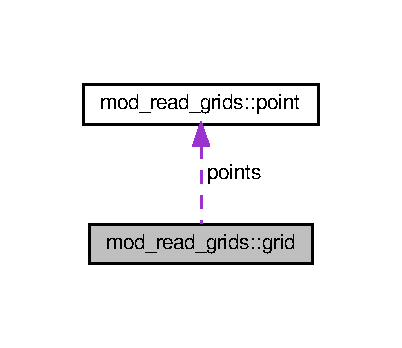
\includegraphics[width=193pt]{structmod__read__grids_1_1grid__coll__graph}
\end{center}
\end{figure}
\subsection*{Public Attributes}
\begin{DoxyCompactItemize}
\item 
type(\hyperlink{structmod__read__grids_1_1point}{point}), dimension(\+:), allocatable \hyperlink{structmod__read__grids_1_1grid_aa276c61a9bfda811d98102170e4bfeaf}{points}
\item 
integer \hyperlink{structmod__read__grids_1_1grid_a71e57f105913758d04222ff4a0a33c5e}{numpoint}
\end{DoxyCompactItemize}


\subsection{Detailed Description}


Definition at line 26 of file mod\+\_\+read\+\_\+grids.\+f90.



\subsection{Member Data Documentation}
\index{mod\+\_\+read\+\_\+grids\+::grid@{mod\+\_\+read\+\_\+grids\+::grid}!numpoint@{numpoint}}
\index{numpoint@{numpoint}!mod\+\_\+read\+\_\+grids\+::grid@{mod\+\_\+read\+\_\+grids\+::grid}}
\subsubsection[{\texorpdfstring{numpoint}{numpoint}}]{\setlength{\rightskip}{0pt plus 5cm}integer mod\+\_\+read\+\_\+grids\+::grid\+::numpoint}\hypertarget{structmod__read__grids_1_1grid_a71e57f105913758d04222ff4a0a33c5e}{}\label{structmod__read__grids_1_1grid_a71e57f105913758d04222ff4a0a33c5e}


Definition at line 28 of file mod\+\_\+read\+\_\+grids.\+f90.

\index{mod\+\_\+read\+\_\+grids\+::grid@{mod\+\_\+read\+\_\+grids\+::grid}!points@{points}}
\index{points@{points}!mod\+\_\+read\+\_\+grids\+::grid@{mod\+\_\+read\+\_\+grids\+::grid}}
\subsubsection[{\texorpdfstring{points}{points}}]{\setlength{\rightskip}{0pt plus 5cm}type( {\bf point} ), dimension(\+:), allocatable mod\+\_\+read\+\_\+grids\+::grid\+::points}\hypertarget{structmod__read__grids_1_1grid_aa276c61a9bfda811d98102170e4bfeaf}{}\label{structmod__read__grids_1_1grid_aa276c61a9bfda811d98102170e4bfeaf}


Definition at line 27 of file mod\+\_\+read\+\_\+grids.\+f90.



The documentation for this type was generated from the following file\+:\begin{DoxyCompactItemize}
\item 
/home/alozada/\+T\+H\+E\+M\+I\+S-\/\+D\+E\+V/themis-\/dev/code/src/\hyperlink{mod__read__grids_8f90}{mod\+\_\+read\+\_\+grids.\+f90}\end{DoxyCompactItemize}

\hypertarget{structmod__pot__ljc_1_1ljc__atom}{}\section{mod\+\_\+pot\+\_\+ljc\+:\+:ljc\+\_\+atom Type Reference}
\label{structmod__pot__ljc_1_1ljc__atom}\index{mod\+\_\+pot\+\_\+ljc\+::ljc\+\_\+atom@{mod\+\_\+pot\+\_\+ljc\+::ljc\+\_\+atom}}


Inheritance diagram for mod\+\_\+pot\+\_\+ljc\+:\+:ljc\+\_\+atom\+:\nopagebreak
\begin{figure}[H]
\begin{center}
\leavevmode
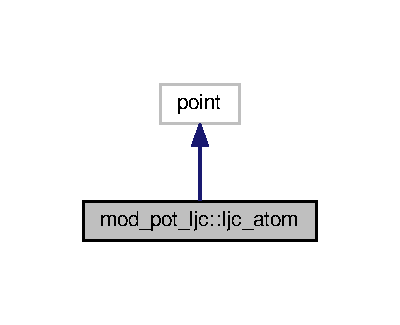
\includegraphics[width=192pt]{structmod__pot__ljc_1_1ljc__atom__inherit__graph}
\end{center}
\end{figure}


Collaboration diagram for mod\+\_\+pot\+\_\+ljc\+:\+:ljc\+\_\+atom\+:\nopagebreak
\begin{figure}[H]
\begin{center}
\leavevmode
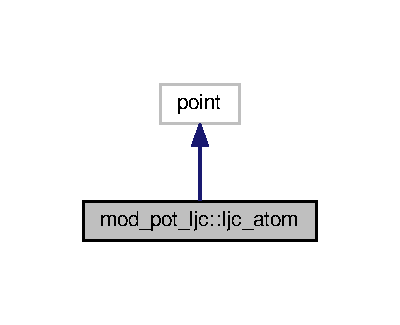
\includegraphics[width=192pt]{structmod__pot__ljc_1_1ljc__atom__coll__graph}
\end{center}
\end{figure}
\subsection*{Public Attributes}
\begin{DoxyCompactItemize}
\item 
real(kind=dp) \hyperlink{structmod__pot__ljc_1_1ljc__atom_a94e32d61122a45a46b7f0d82c0e13c40}{q}
\item 
real(kind=dp) \hyperlink{structmod__pot__ljc_1_1ljc__atom_a2213de956be81f40a4c158a873058040}{sig}
\item 
real(kind=dp) \hyperlink{structmod__pot__ljc_1_1ljc__atom_a9c100db84a17fb8ba3e048b0f7c5fcce}{eps}
\end{DoxyCompactItemize}


\subsection{Detailed Description}


Definition at line 18 of file mod\+\_\+pot\+\_\+ljc.\+f90.



\subsection{Member Data Documentation}
\index{mod\+\_\+pot\+\_\+ljc\+::ljc\+\_\+atom@{mod\+\_\+pot\+\_\+ljc\+::ljc\+\_\+atom}!eps@{eps}}
\index{eps@{eps}!mod\+\_\+pot\+\_\+ljc\+::ljc\+\_\+atom@{mod\+\_\+pot\+\_\+ljc\+::ljc\+\_\+atom}}
\subsubsection[{\texorpdfstring{eps}{eps}}]{\setlength{\rightskip}{0pt plus 5cm}real( kind = dp ) mod\+\_\+pot\+\_\+ljc\+::ljc\+\_\+atom\+::eps}\hypertarget{structmod__pot__ljc_1_1ljc__atom_a9c100db84a17fb8ba3e048b0f7c5fcce}{}\label{structmod__pot__ljc_1_1ljc__atom_a9c100db84a17fb8ba3e048b0f7c5fcce}


Definition at line 19 of file mod\+\_\+pot\+\_\+ljc.\+f90.

\index{mod\+\_\+pot\+\_\+ljc\+::ljc\+\_\+atom@{mod\+\_\+pot\+\_\+ljc\+::ljc\+\_\+atom}!q@{q}}
\index{q@{q}!mod\+\_\+pot\+\_\+ljc\+::ljc\+\_\+atom@{mod\+\_\+pot\+\_\+ljc\+::ljc\+\_\+atom}}
\subsubsection[{\texorpdfstring{q}{q}}]{\setlength{\rightskip}{0pt plus 5cm}real( kind = dp ) mod\+\_\+pot\+\_\+ljc\+::ljc\+\_\+atom\+::q}\hypertarget{structmod__pot__ljc_1_1ljc__atom_a94e32d61122a45a46b7f0d82c0e13c40}{}\label{structmod__pot__ljc_1_1ljc__atom_a94e32d61122a45a46b7f0d82c0e13c40}


Definition at line 19 of file mod\+\_\+pot\+\_\+ljc.\+f90.

\index{mod\+\_\+pot\+\_\+ljc\+::ljc\+\_\+atom@{mod\+\_\+pot\+\_\+ljc\+::ljc\+\_\+atom}!sig@{sig}}
\index{sig@{sig}!mod\+\_\+pot\+\_\+ljc\+::ljc\+\_\+atom@{mod\+\_\+pot\+\_\+ljc\+::ljc\+\_\+atom}}
\subsubsection[{\texorpdfstring{sig}{sig}}]{\setlength{\rightskip}{0pt plus 5cm}real( kind = dp ) mod\+\_\+pot\+\_\+ljc\+::ljc\+\_\+atom\+::sig}\hypertarget{structmod__pot__ljc_1_1ljc__atom_a2213de956be81f40a4c158a873058040}{}\label{structmod__pot__ljc_1_1ljc__atom_a2213de956be81f40a4c158a873058040}


Definition at line 19 of file mod\+\_\+pot\+\_\+ljc.\+f90.



The documentation for this type was generated from the following file\+:\begin{DoxyCompactItemize}
\item 
/home/alozada/\+T\+H\+E\+M\+I\+S-\/\+D\+E\+V/themis-\/dev/code/src/\hyperlink{mod__pot__ljc_8f90}{mod\+\_\+pot\+\_\+ljc.\+f90}\end{DoxyCompactItemize}

\hypertarget{structmod__pot__ljc_1_1ljc__mol}{}\section{mod\+\_\+pot\+\_\+ljc\+:\+:ljc\+\_\+mol Type Reference}
\label{structmod__pot__ljc_1_1ljc__mol}\index{mod\+\_\+pot\+\_\+ljc\+::ljc\+\_\+mol@{mod\+\_\+pot\+\_\+ljc\+::ljc\+\_\+mol}}


Inheritance diagram for mod\+\_\+pot\+\_\+ljc\+:\+:ljc\+\_\+mol\+:\nopagebreak
\begin{figure}[H]
\begin{center}
\leavevmode
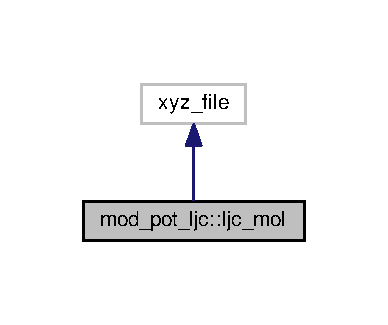
\includegraphics[width=186pt]{structmod__pot__ljc_1_1ljc__mol__inherit__graph}
\end{center}
\end{figure}


Collaboration diagram for mod\+\_\+pot\+\_\+ljc\+:\+:ljc\+\_\+mol\+:\nopagebreak
\begin{figure}[H]
\begin{center}
\leavevmode
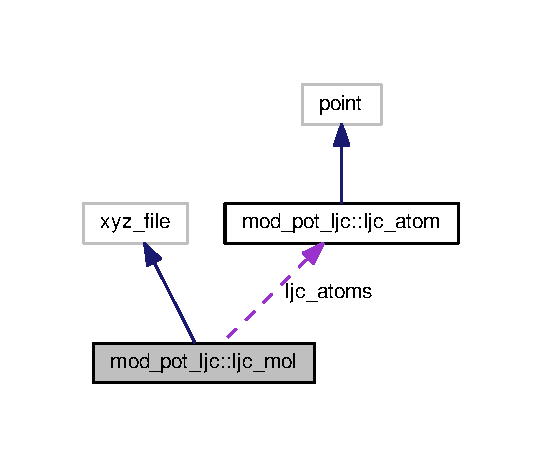
\includegraphics[width=260pt]{structmod__pot__ljc_1_1ljc__mol__coll__graph}
\end{center}
\end{figure}
\subsection*{Public Member Functions}
\begin{DoxyCompactItemize}
\item 
procedure \hyperlink{structmod__pot__ljc_1_1ljc__mol_ace8e9826de989061f30b31cc0e72c248}{read\+\_\+ljc\+\_\+params}
\item 
procedure \hyperlink{structmod__pot__ljc_1_1ljc__mol_af2b424674b36a1beea7d81374e3d3890}{check\+\_\+ljc\+\_\+params}
\end{DoxyCompactItemize}
\subsection*{Public Attributes}
\begin{DoxyCompactItemize}
\item 
type(\hyperlink{structmod__pot__ljc_1_1ljc__atom}{ljc\+\_\+atom}), dimension(\+:), allocatable \hyperlink{structmod__pot__ljc_1_1ljc__mol_a65026a4645ff0576b8a7189649b47512}{ljc\+\_\+atoms}
\end{DoxyCompactItemize}


\subsection{Detailed Description}


Definition at line 22 of file mod\+\_\+pot\+\_\+ljc.\+f90.



\subsection{Member Function/\+Subroutine Documentation}
\index{mod\+\_\+pot\+\_\+ljc\+::ljc\+\_\+mol@{mod\+\_\+pot\+\_\+ljc\+::ljc\+\_\+mol}!check\+\_\+ljc\+\_\+params@{check\+\_\+ljc\+\_\+params}}
\index{check\+\_\+ljc\+\_\+params@{check\+\_\+ljc\+\_\+params}!mod\+\_\+pot\+\_\+ljc\+::ljc\+\_\+mol@{mod\+\_\+pot\+\_\+ljc\+::ljc\+\_\+mol}}
\subsubsection[{\texorpdfstring{check\+\_\+ljc\+\_\+params}{check_ljc_params}}]{\setlength{\rightskip}{0pt plus 5cm}procedure mod\+\_\+pot\+\_\+ljc\+::ljc\+\_\+mol\+::check\+\_\+ljc\+\_\+params (
\begin{DoxyParamCaption}
{}
\end{DoxyParamCaption}
)}\hypertarget{structmod__pot__ljc_1_1ljc__mol_af2b424674b36a1beea7d81374e3d3890}{}\label{structmod__pot__ljc_1_1ljc__mol_af2b424674b36a1beea7d81374e3d3890}


Definition at line 26 of file mod\+\_\+pot\+\_\+ljc.\+f90.

\index{mod\+\_\+pot\+\_\+ljc\+::ljc\+\_\+mol@{mod\+\_\+pot\+\_\+ljc\+::ljc\+\_\+mol}!read\+\_\+ljc\+\_\+params@{read\+\_\+ljc\+\_\+params}}
\index{read\+\_\+ljc\+\_\+params@{read\+\_\+ljc\+\_\+params}!mod\+\_\+pot\+\_\+ljc\+::ljc\+\_\+mol@{mod\+\_\+pot\+\_\+ljc\+::ljc\+\_\+mol}}
\subsubsection[{\texorpdfstring{read\+\_\+ljc\+\_\+params}{read_ljc_params}}]{\setlength{\rightskip}{0pt plus 5cm}procedure mod\+\_\+pot\+\_\+ljc\+::ljc\+\_\+mol\+::read\+\_\+ljc\+\_\+params (
\begin{DoxyParamCaption}
{}
\end{DoxyParamCaption}
)}\hypertarget{structmod__pot__ljc_1_1ljc__mol_ace8e9826de989061f30b31cc0e72c248}{}\label{structmod__pot__ljc_1_1ljc__mol_ace8e9826de989061f30b31cc0e72c248}


Definition at line 25 of file mod\+\_\+pot\+\_\+ljc.\+f90.



\subsection{Member Data Documentation}
\index{mod\+\_\+pot\+\_\+ljc\+::ljc\+\_\+mol@{mod\+\_\+pot\+\_\+ljc\+::ljc\+\_\+mol}!ljc\+\_\+atoms@{ljc\+\_\+atoms}}
\index{ljc\+\_\+atoms@{ljc\+\_\+atoms}!mod\+\_\+pot\+\_\+ljc\+::ljc\+\_\+mol@{mod\+\_\+pot\+\_\+ljc\+::ljc\+\_\+mol}}
\subsubsection[{\texorpdfstring{ljc\+\_\+atoms}{ljc_atoms}}]{\setlength{\rightskip}{0pt plus 5cm}type( {\bf ljc\+\_\+atom} ), dimension(\+:), allocatable mod\+\_\+pot\+\_\+ljc\+::ljc\+\_\+mol\+::ljc\+\_\+atoms}\hypertarget{structmod__pot__ljc_1_1ljc__mol_a65026a4645ff0576b8a7189649b47512}{}\label{structmod__pot__ljc_1_1ljc__mol_a65026a4645ff0576b8a7189649b47512}


Definition at line 23 of file mod\+\_\+pot\+\_\+ljc.\+f90.



The documentation for this type was generated from the following file\+:\begin{DoxyCompactItemize}
\item 
/home/alozada/\+T\+H\+E\+M\+I\+S-\/\+D\+E\+V/themis-\/dev/code/src/\hyperlink{mod__pot__ljc_8f90}{mod\+\_\+pot\+\_\+ljc.\+f90}\end{DoxyCompactItemize}

\hypertarget{structmod__read__grids_1_1point}{}\section{mod\+\_\+read\+\_\+grids\+:\+:point Type Reference}
\label{structmod__read__grids_1_1point}\index{mod\+\_\+read\+\_\+grids\+::point@{mod\+\_\+read\+\_\+grids\+::point}}
\subsection*{Public Attributes}
\begin{DoxyCompactItemize}
\item 
real(kind=dp), dimension(3) \hyperlink{structmod__read__grids_1_1point_a44e07983c85907248f16a1d5409902a8}{grid\+\_\+xyz}
\item 
real(kind=dp), dimension(3) \hyperlink{structmod__read__grids_1_1point_a010b9b432e70f8114e6ba80806abc995}{grid\+\_\+xyz\+\_\+old}
\item 
real(kind=dp), dimension(3) \hyperlink{structmod__read__grids_1_1point_ab0f3d5d60468a83f53e8f09bda7b17b3}{grid\+\_\+xyz\+\_\+rot}
\item 
character(len=3) \hyperlink{structmod__read__grids_1_1point_a4eddf2d1dd9848de549cb9e5a54aa333}{grid\+\_\+symbol}
\end{DoxyCompactItemize}


\subsection{Detailed Description}


Definition at line 24 of file mod\+\_\+read\+\_\+grids.\+f90.



\subsection{Member Data Documentation}
\mbox{\Hypertarget{structmod__read__grids_1_1point_a4eddf2d1dd9848de549cb9e5a54aa333}\label{structmod__read__grids_1_1point_a4eddf2d1dd9848de549cb9e5a54aa333}} 
\index{mod\+\_\+read\+\_\+grids\+::point@{mod\+\_\+read\+\_\+grids\+::point}!grid\+\_\+symbol@{grid\+\_\+symbol}}
\index{grid\+\_\+symbol@{grid\+\_\+symbol}!mod\+\_\+read\+\_\+grids\+::point@{mod\+\_\+read\+\_\+grids\+::point}}
\subsubsection{\texorpdfstring{grid\+\_\+symbol}{grid\_symbol}}
{\footnotesize\ttfamily character( len = 3 ) mod\+\_\+read\+\_\+grids\+::point\+::grid\+\_\+symbol}



Definition at line 26 of file mod\+\_\+read\+\_\+grids.\+f90.

\mbox{\Hypertarget{structmod__read__grids_1_1point_a44e07983c85907248f16a1d5409902a8}\label{structmod__read__grids_1_1point_a44e07983c85907248f16a1d5409902a8}} 
\index{mod\+\_\+read\+\_\+grids\+::point@{mod\+\_\+read\+\_\+grids\+::point}!grid\+\_\+xyz@{grid\+\_\+xyz}}
\index{grid\+\_\+xyz@{grid\+\_\+xyz}!mod\+\_\+read\+\_\+grids\+::point@{mod\+\_\+read\+\_\+grids\+::point}}
\subsubsection{\texorpdfstring{grid\+\_\+xyz}{grid\_xyz}}
{\footnotesize\ttfamily real( kind = dp ), dimension(3) mod\+\_\+read\+\_\+grids\+::point\+::grid\+\_\+xyz}



Definition at line 25 of file mod\+\_\+read\+\_\+grids.\+f90.

\mbox{\Hypertarget{structmod__read__grids_1_1point_a010b9b432e70f8114e6ba80806abc995}\label{structmod__read__grids_1_1point_a010b9b432e70f8114e6ba80806abc995}} 
\index{mod\+\_\+read\+\_\+grids\+::point@{mod\+\_\+read\+\_\+grids\+::point}!grid\+\_\+xyz\+\_\+old@{grid\+\_\+xyz\+\_\+old}}
\index{grid\+\_\+xyz\+\_\+old@{grid\+\_\+xyz\+\_\+old}!mod\+\_\+read\+\_\+grids\+::point@{mod\+\_\+read\+\_\+grids\+::point}}
\subsubsection{\texorpdfstring{grid\+\_\+xyz\+\_\+old}{grid\_xyz\_old}}
{\footnotesize\ttfamily real( kind = dp ), dimension(3) mod\+\_\+read\+\_\+grids\+::point\+::grid\+\_\+xyz\+\_\+old}



Definition at line 25 of file mod\+\_\+read\+\_\+grids.\+f90.

\mbox{\Hypertarget{structmod__read__grids_1_1point_ab0f3d5d60468a83f53e8f09bda7b17b3}\label{structmod__read__grids_1_1point_ab0f3d5d60468a83f53e8f09bda7b17b3}} 
\index{mod\+\_\+read\+\_\+grids\+::point@{mod\+\_\+read\+\_\+grids\+::point}!grid\+\_\+xyz\+\_\+rot@{grid\+\_\+xyz\+\_\+rot}}
\index{grid\+\_\+xyz\+\_\+rot@{grid\+\_\+xyz\+\_\+rot}!mod\+\_\+read\+\_\+grids\+::point@{mod\+\_\+read\+\_\+grids\+::point}}
\subsubsection{\texorpdfstring{grid\+\_\+xyz\+\_\+rot}{grid\_xyz\_rot}}
{\footnotesize\ttfamily real( kind = dp ), dimension(3) mod\+\_\+read\+\_\+grids\+::point\+::grid\+\_\+xyz\+\_\+rot}



Definition at line 25 of file mod\+\_\+read\+\_\+grids.\+f90.



The documentation for this type was generated from the following file\+:\begin{DoxyCompactItemize}
\item 
/home/alozada/\+T\+H\+E\+M\+I\+S\+\_\+\+D\+E\+C\+E\+M\+B\+E\+R/themis-\/dev\+\_\+december/code/src/\hyperlink{mod__read__grids_8f90}{mod\+\_\+read\+\_\+grids.\+f90}\end{DoxyCompactItemize}

\hypertarget{structmod__read__xyz_1_1point}{}\section{mod\+\_\+read\+\_\+xyz\+:\+:point Type Reference}
\label{structmod__read__xyz_1_1point}\index{mod\+\_\+read\+\_\+xyz\+::point@{mod\+\_\+read\+\_\+xyz\+::point}}
\subsection*{Public Attributes}
\begin{DoxyCompactItemize}
\item 
real(kind=dp), dimension(3) \hyperlink{structmod__read__xyz_1_1point_a0f0abb4553673dd53beed006d23e8044}{xyz}
\item 
real(kind=dp), dimension(3) \hyperlink{structmod__read__xyz_1_1point_a850b0992c9c67aa0ab7f0cc5ce6e06a4}{xyz\+\_\+old}
\item 
real(kind=dp), dimension(3) \hyperlink{structmod__read__xyz_1_1point_a8065dc01a4172608ef691b470ad6b781}{xyz\+\_\+rot}
\item 
character(len=3) \hyperlink{structmod__read__xyz_1_1point_a95b7d7fa3c68486c2ea9537fdfd74fb7}{symbol}
\end{DoxyCompactItemize}


\subsection{Detailed Description}


Definition at line 17 of file mod\+\_\+read\+\_\+xyz.\+f90.



\subsection{Member Data Documentation}
\index{mod\+\_\+read\+\_\+xyz\+::point@{mod\+\_\+read\+\_\+xyz\+::point}!symbol@{symbol}}
\index{symbol@{symbol}!mod\+\_\+read\+\_\+xyz\+::point@{mod\+\_\+read\+\_\+xyz\+::point}}
\subsubsection[{\texorpdfstring{symbol}{symbol}}]{\setlength{\rightskip}{0pt plus 5cm}character( len = 3 ) mod\+\_\+read\+\_\+xyz\+::point\+::symbol}\hypertarget{structmod__read__xyz_1_1point_a95b7d7fa3c68486c2ea9537fdfd74fb7}{}\label{structmod__read__xyz_1_1point_a95b7d7fa3c68486c2ea9537fdfd74fb7}


Definition at line 19 of file mod\+\_\+read\+\_\+xyz.\+f90.

\index{mod\+\_\+read\+\_\+xyz\+::point@{mod\+\_\+read\+\_\+xyz\+::point}!xyz@{xyz}}
\index{xyz@{xyz}!mod\+\_\+read\+\_\+xyz\+::point@{mod\+\_\+read\+\_\+xyz\+::point}}
\subsubsection[{\texorpdfstring{xyz}{xyz}}]{\setlength{\rightskip}{0pt plus 5cm}real( kind = dp ), dimension(3) mod\+\_\+read\+\_\+xyz\+::point\+::xyz}\hypertarget{structmod__read__xyz_1_1point_a0f0abb4553673dd53beed006d23e8044}{}\label{structmod__read__xyz_1_1point_a0f0abb4553673dd53beed006d23e8044}


Definition at line 18 of file mod\+\_\+read\+\_\+xyz.\+f90.

\index{mod\+\_\+read\+\_\+xyz\+::point@{mod\+\_\+read\+\_\+xyz\+::point}!xyz\+\_\+old@{xyz\+\_\+old}}
\index{xyz\+\_\+old@{xyz\+\_\+old}!mod\+\_\+read\+\_\+xyz\+::point@{mod\+\_\+read\+\_\+xyz\+::point}}
\subsubsection[{\texorpdfstring{xyz\+\_\+old}{xyz_old}}]{\setlength{\rightskip}{0pt plus 5cm}real( kind = dp ), dimension(3) mod\+\_\+read\+\_\+xyz\+::point\+::xyz\+\_\+old}\hypertarget{structmod__read__xyz_1_1point_a850b0992c9c67aa0ab7f0cc5ce6e06a4}{}\label{structmod__read__xyz_1_1point_a850b0992c9c67aa0ab7f0cc5ce6e06a4}


Definition at line 18 of file mod\+\_\+read\+\_\+xyz.\+f90.

\index{mod\+\_\+read\+\_\+xyz\+::point@{mod\+\_\+read\+\_\+xyz\+::point}!xyz\+\_\+rot@{xyz\+\_\+rot}}
\index{xyz\+\_\+rot@{xyz\+\_\+rot}!mod\+\_\+read\+\_\+xyz\+::point@{mod\+\_\+read\+\_\+xyz\+::point}}
\subsubsection[{\texorpdfstring{xyz\+\_\+rot}{xyz_rot}}]{\setlength{\rightskip}{0pt plus 5cm}real( kind = dp ), dimension(3) mod\+\_\+read\+\_\+xyz\+::point\+::xyz\+\_\+rot}\hypertarget{structmod__read__xyz_1_1point_a8065dc01a4172608ef691b470ad6b781}{}\label{structmod__read__xyz_1_1point_a8065dc01a4172608ef691b470ad6b781}


Definition at line 18 of file mod\+\_\+read\+\_\+xyz.\+f90.



The documentation for this type was generated from the following file\+:\begin{DoxyCompactItemize}
\item 
/home/alozada/\+T\+H\+E\+M\+I\+S-\/\+D\+E\+V/themis-\/dev/code/src/\hyperlink{mod__read__xyz_8f90}{mod\+\_\+read\+\_\+xyz.\+f90}\end{DoxyCompactItemize}

\hypertarget{structxdr_1_1xtcfile}{}\section{xdr\+:\+:xtcfile Type Reference}
\label{structxdr_1_1xtcfile}\index{xdr\+::xtcfile@{xdr\+::xtcfile}}


Inheritance diagram for xdr\+:\+:xtcfile\+:\nopagebreak
\begin{figure}[H]
\begin{center}
\leavevmode
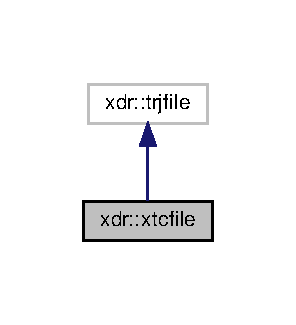
\includegraphics[width=142pt]{structxdr_1_1xtcfile__inherit__graph}
\end{center}
\end{figure}


Collaboration diagram for xdr\+:\+:xtcfile\+:\nopagebreak
\begin{figure}[H]
\begin{center}
\leavevmode
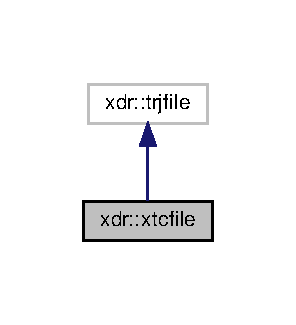
\includegraphics[width=142pt]{structxdr_1_1xtcfile__coll__graph}
\end{center}
\end{figure}
\subsection*{Public Member Functions}
\begin{DoxyCompactItemize}
\item 
procedure \hyperlink{structxdr_1_1xtcfile_ac2af78519ced579714c7ffe4f15f5d46}{write} =$>$ write\+\_\+xtcfile
\end{DoxyCompactItemize}
\subsection*{Public Attributes}
\begin{DoxyCompactItemize}
\item 
real(c\+\_\+float), dimension(3, 3) \hyperlink{structxdr_1_1xtcfile_a7472d3a09f388bc3f95b74a289b994ad}{box}
\item 
real(c\+\_\+float) \hyperlink{structxdr_1_1xtcfile_a8bbfbd475a67d143c56584ec6adc5851}{time}
\item 
real(c\+\_\+float), dimension(\+:,\+:), allocatable \hyperlink{structxdr_1_1xtcfile_abda2627be95e0de9df18e915d53a988a}{pos}
\item 
real(c\+\_\+float) \hyperlink{structxdr_1_1xtcfile_aac421da0ff0c236f762eb81f1b726c2f}{prec}
\end{DoxyCompactItemize}


\subsection{Detailed Description}


Definition at line 50 of file xdr.\+f90.



\subsection{Member Function/\+Subroutine Documentation}
\index{xdr\+::xtcfile@{xdr\+::xtcfile}!write@{write}}
\index{write@{write}!xdr\+::xtcfile@{xdr\+::xtcfile}}
\subsubsection[{\texorpdfstring{write=$>$ write\+\_\+xtcfile}{write=> write_xtcfile}}]{\setlength{\rightskip}{0pt plus 5cm}procedure xdr\+::xtcfile\+::write (
\begin{DoxyParamCaption}
{}
\end{DoxyParamCaption}
)}\hypertarget{structxdr_1_1xtcfile_ac2af78519ced579714c7ffe4f15f5d46}{}\label{structxdr_1_1xtcfile_ac2af78519ced579714c7ffe4f15f5d46}


Definition at line 55 of file xdr.\+f90.



\subsection{Member Data Documentation}
\index{xdr\+::xtcfile@{xdr\+::xtcfile}!box@{box}}
\index{box@{box}!xdr\+::xtcfile@{xdr\+::xtcfile}}
\subsubsection[{\texorpdfstring{box}{box}}]{\setlength{\rightskip}{0pt plus 5cm}real(c\+\_\+float), dimension(3, 3) xdr\+::xtcfile\+::box}\hypertarget{structxdr_1_1xtcfile_a7472d3a09f388bc3f95b74a289b994ad}{}\label{structxdr_1_1xtcfile_a7472d3a09f388bc3f95b74a289b994ad}


Definition at line 51 of file xdr.\+f90.

\index{xdr\+::xtcfile@{xdr\+::xtcfile}!pos@{pos}}
\index{pos@{pos}!xdr\+::xtcfile@{xdr\+::xtcfile}}
\subsubsection[{\texorpdfstring{pos}{pos}}]{\setlength{\rightskip}{0pt plus 5cm}real(c\+\_\+float), dimension(\+:, \+:), allocatable xdr\+::xtcfile\+::pos}\hypertarget{structxdr_1_1xtcfile_abda2627be95e0de9df18e915d53a988a}{}\label{structxdr_1_1xtcfile_abda2627be95e0de9df18e915d53a988a}


Definition at line 52 of file xdr.\+f90.

\index{xdr\+::xtcfile@{xdr\+::xtcfile}!prec@{prec}}
\index{prec@{prec}!xdr\+::xtcfile@{xdr\+::xtcfile}}
\subsubsection[{\texorpdfstring{prec}{prec}}]{\setlength{\rightskip}{0pt plus 5cm}real(c\+\_\+float) xdr\+::xtcfile\+::prec}\hypertarget{structxdr_1_1xtcfile_aac421da0ff0c236f762eb81f1b726c2f}{}\label{structxdr_1_1xtcfile_aac421da0ff0c236f762eb81f1b726c2f}


Definition at line 53 of file xdr.\+f90.

\index{xdr\+::xtcfile@{xdr\+::xtcfile}!time@{time}}
\index{time@{time}!xdr\+::xtcfile@{xdr\+::xtcfile}}
\subsubsection[{\texorpdfstring{time}{time}}]{\setlength{\rightskip}{0pt plus 5cm}real(c\+\_\+float) xdr\+::xtcfile\+::time}\hypertarget{structxdr_1_1xtcfile_a8bbfbd475a67d143c56584ec6adc5851}{}\label{structxdr_1_1xtcfile_a8bbfbd475a67d143c56584ec6adc5851}


Definition at line 51 of file xdr.\+f90.



The documentation for this type was generated from the following file\+:\begin{DoxyCompactItemize}
\item 
/home/alozada/\+T\+H\+E\+M\+I\+S-\/\+D\+E\+V/themis-\/dev/code/src/\hyperlink{xdr_8f90}{xdr.\+f90}\end{DoxyCompactItemize}

\hypertarget{structmod__read__xyz_1_1xyz__dimer}{}\section{mod\+\_\+read\+\_\+xyz\+:\+:xyz\+\_\+dimer Type Reference}
\label{structmod__read__xyz_1_1xyz__dimer}\index{mod\+\_\+read\+\_\+xyz\+::xyz\+\_\+dimer@{mod\+\_\+read\+\_\+xyz\+::xyz\+\_\+dimer}}


Collaboration diagram for mod\+\_\+read\+\_\+xyz\+:\+:xyz\+\_\+dimer\+:\nopagebreak
\begin{figure}[H]
\begin{center}
\leavevmode
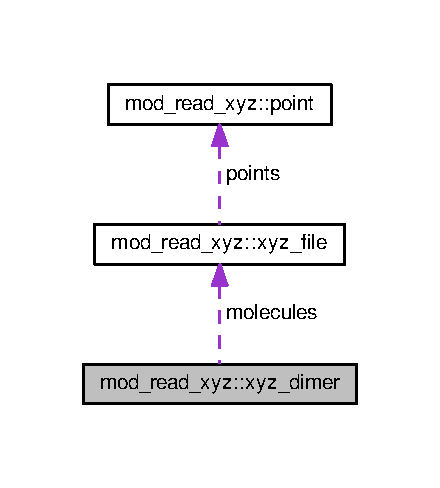
\includegraphics[width=211pt]{structmod__read__xyz_1_1xyz__dimer__coll__graph}
\end{center}
\end{figure}
\subsection*{Public Member Functions}
\begin{DoxyCompactItemize}
\item 
procedure, pass \hyperlink{structmod__read__xyz_1_1xyz__dimer_ad0dbe3dddad53d4031df233102327f8c}{build\+\_\+dimer}
\item 
procedure, pass \hyperlink{structmod__read__xyz_1_1xyz__dimer_a452b6927d8e712dd73467dd57b9141d8}{write\+\_\+xyz}
\end{DoxyCompactItemize}
\subsection*{Public Attributes}
\begin{DoxyCompactItemize}
\item 
type(\hyperlink{structmod__read__xyz_1_1xyz__file}{xyz\+\_\+file}), dimension(2) \hyperlink{structmod__read__xyz_1_1xyz__dimer_af7e03e5b57bc4a39e4905ff0aecbf6b6}{molecules}
\end{DoxyCompactItemize}


\subsection{Detailed Description}


Definition at line 35 of file mod\+\_\+read\+\_\+xyz.\+f90.



\subsection{Member Function/\+Subroutine Documentation}
\index{mod\+\_\+read\+\_\+xyz\+::xyz\+\_\+dimer@{mod\+\_\+read\+\_\+xyz\+::xyz\+\_\+dimer}!build\+\_\+dimer@{build\+\_\+dimer}}
\index{build\+\_\+dimer@{build\+\_\+dimer}!mod\+\_\+read\+\_\+xyz\+::xyz\+\_\+dimer@{mod\+\_\+read\+\_\+xyz\+::xyz\+\_\+dimer}}
\subsubsection[{\texorpdfstring{build\+\_\+dimer}{build_dimer}}]{\setlength{\rightskip}{0pt plus 5cm}procedure, pass mod\+\_\+read\+\_\+xyz\+::xyz\+\_\+dimer\+::build\+\_\+dimer (
\begin{DoxyParamCaption}
{}
\end{DoxyParamCaption}
)}\hypertarget{structmod__read__xyz_1_1xyz__dimer_ad0dbe3dddad53d4031df233102327f8c}{}\label{structmod__read__xyz_1_1xyz__dimer_ad0dbe3dddad53d4031df233102327f8c}


Definition at line 38 of file mod\+\_\+read\+\_\+xyz.\+f90.

\index{mod\+\_\+read\+\_\+xyz\+::xyz\+\_\+dimer@{mod\+\_\+read\+\_\+xyz\+::xyz\+\_\+dimer}!write\+\_\+xyz@{write\+\_\+xyz}}
\index{write\+\_\+xyz@{write\+\_\+xyz}!mod\+\_\+read\+\_\+xyz\+::xyz\+\_\+dimer@{mod\+\_\+read\+\_\+xyz\+::xyz\+\_\+dimer}}
\subsubsection[{\texorpdfstring{write\+\_\+xyz}{write_xyz}}]{\setlength{\rightskip}{0pt plus 5cm}procedure, pass mod\+\_\+read\+\_\+xyz\+::xyz\+\_\+dimer\+::write\+\_\+xyz (
\begin{DoxyParamCaption}
{}
\end{DoxyParamCaption}
)}\hypertarget{structmod__read__xyz_1_1xyz__dimer_a452b6927d8e712dd73467dd57b9141d8}{}\label{structmod__read__xyz_1_1xyz__dimer_a452b6927d8e712dd73467dd57b9141d8}


Definition at line 39 of file mod\+\_\+read\+\_\+xyz.\+f90.



\subsection{Member Data Documentation}
\index{mod\+\_\+read\+\_\+xyz\+::xyz\+\_\+dimer@{mod\+\_\+read\+\_\+xyz\+::xyz\+\_\+dimer}!molecules@{molecules}}
\index{molecules@{molecules}!mod\+\_\+read\+\_\+xyz\+::xyz\+\_\+dimer@{mod\+\_\+read\+\_\+xyz\+::xyz\+\_\+dimer}}
\subsubsection[{\texorpdfstring{molecules}{molecules}}]{\setlength{\rightskip}{0pt plus 5cm}type( {\bf xyz\+\_\+file} ), dimension(2) mod\+\_\+read\+\_\+xyz\+::xyz\+\_\+dimer\+::molecules}\hypertarget{structmod__read__xyz_1_1xyz__dimer_af7e03e5b57bc4a39e4905ff0aecbf6b6}{}\label{structmod__read__xyz_1_1xyz__dimer_af7e03e5b57bc4a39e4905ff0aecbf6b6}


Definition at line 36 of file mod\+\_\+read\+\_\+xyz.\+f90.



The documentation for this type was generated from the following file\+:\begin{DoxyCompactItemize}
\item 
/home/alozada/\+T\+H\+E\+M\+I\+S-\/\+D\+E\+V/themis-\/dev/code/src/\hyperlink{mod__read__xyz_8f90}{mod\+\_\+read\+\_\+xyz.\+f90}\end{DoxyCompactItemize}

\hypertarget{structmod__read__xyz_1_1xyz__file}{}\section{mod\+\_\+read\+\_\+xyz\+:\+:xyz\+\_\+file Type Reference}
\label{structmod__read__xyz_1_1xyz__file}\index{mod\+\_\+read\+\_\+xyz\+::xyz\+\_\+file@{mod\+\_\+read\+\_\+xyz\+::xyz\+\_\+file}}


Collaboration diagram for mod\+\_\+read\+\_\+xyz\+:\+:xyz\+\_\+file\+:\nopagebreak
\begin{figure}[H]
\begin{center}
\leavevmode
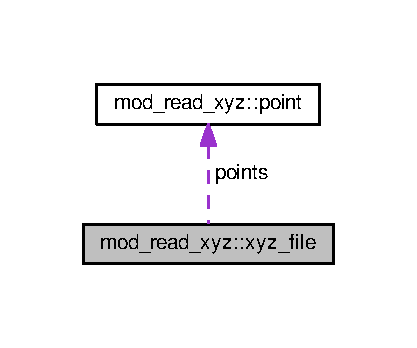
\includegraphics[width=200pt]{structmod__read__xyz_1_1xyz__file__coll__graph}
\end{center}
\end{figure}
\subsection*{Public Member Functions}
\begin{DoxyCompactItemize}
\item 
procedure, pass \hyperlink{structmod__read__xyz_1_1xyz__file_aa11ebdf72bd3cefbb34be37cf4e7d7c3}{read\+\_\+xyz}
\item 
procedure, pass \hyperlink{structmod__read__xyz_1_1xyz__file_a5b5040936c65ef3bffa575589d3832e1}{translate\+\_\+xyz}
\item 
procedure, pass \hyperlink{structmod__read__xyz_1_1xyz__file_ad6d787ad066497b2f341190475842597}{align\+\_\+xyz}
\item 
procedure, pass \hyperlink{structmod__read__xyz_1_1xyz__file_a21ba9b56ce2408f5a61646e39cbcf285}{rotate\+\_\+xyz}
\end{DoxyCompactItemize}
\subsection*{Public Attributes}
\begin{DoxyCompactItemize}
\item 
type(\hyperlink{structmod__read__xyz_1_1point}{point}), dimension(\+:), allocatable \hyperlink{structmod__read__xyz_1_1xyz__file_a918bc6a941d85d90419f1d2c6585224e}{points}
\item 
real(kind=dp), dimension(3) \hyperlink{structmod__read__xyz_1_1xyz__file_a3fc6d7b23f156adb7d7ffa9aa3f3913f}{points\+\_\+center}
\item 
real(kind=dp), dimension(3) \hyperlink{structmod__read__xyz_1_1xyz__file_a333fe3200ebdabc41ff195c6b0a91932}{points\+\_\+vector}
\item 
real(kind=dp) \hyperlink{structmod__read__xyz_1_1xyz__file_ab662f528be048fc7efd32495633a246b}{rot\+\_\+vector}
\item 
integer \hyperlink{structmod__read__xyz_1_1xyz__file_aa338247cd4ff55ae9fe9a2143fe28cdf}{num\+\_\+points}
\end{DoxyCompactItemize}


\subsection{Detailed Description}


Definition at line 22 of file mod\+\_\+read\+\_\+xyz.\+f90.



\subsection{Member Function/\+Subroutine Documentation}
\index{mod\+\_\+read\+\_\+xyz\+::xyz\+\_\+file@{mod\+\_\+read\+\_\+xyz\+::xyz\+\_\+file}!align\+\_\+xyz@{align\+\_\+xyz}}
\index{align\+\_\+xyz@{align\+\_\+xyz}!mod\+\_\+read\+\_\+xyz\+::xyz\+\_\+file@{mod\+\_\+read\+\_\+xyz\+::xyz\+\_\+file}}
\subsubsection[{\texorpdfstring{align\+\_\+xyz}{align_xyz}}]{\setlength{\rightskip}{0pt plus 5cm}procedure, pass mod\+\_\+read\+\_\+xyz\+::xyz\+\_\+file\+::align\+\_\+xyz (
\begin{DoxyParamCaption}
{}
\end{DoxyParamCaption}
)}\hypertarget{structmod__read__xyz_1_1xyz__file_ad6d787ad066497b2f341190475842597}{}\label{structmod__read__xyz_1_1xyz__file_ad6d787ad066497b2f341190475842597}


Definition at line 29 of file mod\+\_\+read\+\_\+xyz.\+f90.

\index{mod\+\_\+read\+\_\+xyz\+::xyz\+\_\+file@{mod\+\_\+read\+\_\+xyz\+::xyz\+\_\+file}!read\+\_\+xyz@{read\+\_\+xyz}}
\index{read\+\_\+xyz@{read\+\_\+xyz}!mod\+\_\+read\+\_\+xyz\+::xyz\+\_\+file@{mod\+\_\+read\+\_\+xyz\+::xyz\+\_\+file}}
\subsubsection[{\texorpdfstring{read\+\_\+xyz}{read_xyz}}]{\setlength{\rightskip}{0pt plus 5cm}procedure, pass mod\+\_\+read\+\_\+xyz\+::xyz\+\_\+file\+::read\+\_\+xyz (
\begin{DoxyParamCaption}
{}
\end{DoxyParamCaption}
)}\hypertarget{structmod__read__xyz_1_1xyz__file_aa11ebdf72bd3cefbb34be37cf4e7d7c3}{}\label{structmod__read__xyz_1_1xyz__file_aa11ebdf72bd3cefbb34be37cf4e7d7c3}


Definition at line 27 of file mod\+\_\+read\+\_\+xyz.\+f90.

\index{mod\+\_\+read\+\_\+xyz\+::xyz\+\_\+file@{mod\+\_\+read\+\_\+xyz\+::xyz\+\_\+file}!rotate\+\_\+xyz@{rotate\+\_\+xyz}}
\index{rotate\+\_\+xyz@{rotate\+\_\+xyz}!mod\+\_\+read\+\_\+xyz\+::xyz\+\_\+file@{mod\+\_\+read\+\_\+xyz\+::xyz\+\_\+file}}
\subsubsection[{\texorpdfstring{rotate\+\_\+xyz}{rotate_xyz}}]{\setlength{\rightskip}{0pt plus 5cm}procedure, pass mod\+\_\+read\+\_\+xyz\+::xyz\+\_\+file\+::rotate\+\_\+xyz (
\begin{DoxyParamCaption}
{}
\end{DoxyParamCaption}
)}\hypertarget{structmod__read__xyz_1_1xyz__file_a21ba9b56ce2408f5a61646e39cbcf285}{}\label{structmod__read__xyz_1_1xyz__file_a21ba9b56ce2408f5a61646e39cbcf285}


Definition at line 30 of file mod\+\_\+read\+\_\+xyz.\+f90.

\index{mod\+\_\+read\+\_\+xyz\+::xyz\+\_\+file@{mod\+\_\+read\+\_\+xyz\+::xyz\+\_\+file}!translate\+\_\+xyz@{translate\+\_\+xyz}}
\index{translate\+\_\+xyz@{translate\+\_\+xyz}!mod\+\_\+read\+\_\+xyz\+::xyz\+\_\+file@{mod\+\_\+read\+\_\+xyz\+::xyz\+\_\+file}}
\subsubsection[{\texorpdfstring{translate\+\_\+xyz}{translate_xyz}}]{\setlength{\rightskip}{0pt plus 5cm}procedure, pass mod\+\_\+read\+\_\+xyz\+::xyz\+\_\+file\+::translate\+\_\+xyz (
\begin{DoxyParamCaption}
{}
\end{DoxyParamCaption}
)}\hypertarget{structmod__read__xyz_1_1xyz__file_a5b5040936c65ef3bffa575589d3832e1}{}\label{structmod__read__xyz_1_1xyz__file_a5b5040936c65ef3bffa575589d3832e1}


Definition at line 28 of file mod\+\_\+read\+\_\+xyz.\+f90.



\subsection{Member Data Documentation}
\index{mod\+\_\+read\+\_\+xyz\+::xyz\+\_\+file@{mod\+\_\+read\+\_\+xyz\+::xyz\+\_\+file}!num\+\_\+points@{num\+\_\+points}}
\index{num\+\_\+points@{num\+\_\+points}!mod\+\_\+read\+\_\+xyz\+::xyz\+\_\+file@{mod\+\_\+read\+\_\+xyz\+::xyz\+\_\+file}}
\subsubsection[{\texorpdfstring{num\+\_\+points}{num_points}}]{\setlength{\rightskip}{0pt plus 5cm}integer mod\+\_\+read\+\_\+xyz\+::xyz\+\_\+file\+::num\+\_\+points}\hypertarget{structmod__read__xyz_1_1xyz__file_aa338247cd4ff55ae9fe9a2143fe28cdf}{}\label{structmod__read__xyz_1_1xyz__file_aa338247cd4ff55ae9fe9a2143fe28cdf}


Definition at line 25 of file mod\+\_\+read\+\_\+xyz.\+f90.

\index{mod\+\_\+read\+\_\+xyz\+::xyz\+\_\+file@{mod\+\_\+read\+\_\+xyz\+::xyz\+\_\+file}!points@{points}}
\index{points@{points}!mod\+\_\+read\+\_\+xyz\+::xyz\+\_\+file@{mod\+\_\+read\+\_\+xyz\+::xyz\+\_\+file}}
\subsubsection[{\texorpdfstring{points}{points}}]{\setlength{\rightskip}{0pt plus 5cm}type( {\bf point} ), dimension(\+:), allocatable mod\+\_\+read\+\_\+xyz\+::xyz\+\_\+file\+::points}\hypertarget{structmod__read__xyz_1_1xyz__file_a918bc6a941d85d90419f1d2c6585224e}{}\label{structmod__read__xyz_1_1xyz__file_a918bc6a941d85d90419f1d2c6585224e}


Definition at line 23 of file mod\+\_\+read\+\_\+xyz.\+f90.

\index{mod\+\_\+read\+\_\+xyz\+::xyz\+\_\+file@{mod\+\_\+read\+\_\+xyz\+::xyz\+\_\+file}!points\+\_\+center@{points\+\_\+center}}
\index{points\+\_\+center@{points\+\_\+center}!mod\+\_\+read\+\_\+xyz\+::xyz\+\_\+file@{mod\+\_\+read\+\_\+xyz\+::xyz\+\_\+file}}
\subsubsection[{\texorpdfstring{points\+\_\+center}{points_center}}]{\setlength{\rightskip}{0pt plus 5cm}real( kind = dp ), dimension(3) mod\+\_\+read\+\_\+xyz\+::xyz\+\_\+file\+::points\+\_\+center}\hypertarget{structmod__read__xyz_1_1xyz__file_a3fc6d7b23f156adb7d7ffa9aa3f3913f}{}\label{structmod__read__xyz_1_1xyz__file_a3fc6d7b23f156adb7d7ffa9aa3f3913f}


Definition at line 24 of file mod\+\_\+read\+\_\+xyz.\+f90.

\index{mod\+\_\+read\+\_\+xyz\+::xyz\+\_\+file@{mod\+\_\+read\+\_\+xyz\+::xyz\+\_\+file}!points\+\_\+vector@{points\+\_\+vector}}
\index{points\+\_\+vector@{points\+\_\+vector}!mod\+\_\+read\+\_\+xyz\+::xyz\+\_\+file@{mod\+\_\+read\+\_\+xyz\+::xyz\+\_\+file}}
\subsubsection[{\texorpdfstring{points\+\_\+vector}{points_vector}}]{\setlength{\rightskip}{0pt plus 5cm}real( kind = dp ), dimension(3) mod\+\_\+read\+\_\+xyz\+::xyz\+\_\+file\+::points\+\_\+vector}\hypertarget{structmod__read__xyz_1_1xyz__file_a333fe3200ebdabc41ff195c6b0a91932}{}\label{structmod__read__xyz_1_1xyz__file_a333fe3200ebdabc41ff195c6b0a91932}


Definition at line 24 of file mod\+\_\+read\+\_\+xyz.\+f90.

\index{mod\+\_\+read\+\_\+xyz\+::xyz\+\_\+file@{mod\+\_\+read\+\_\+xyz\+::xyz\+\_\+file}!rot\+\_\+vector@{rot\+\_\+vector}}
\index{rot\+\_\+vector@{rot\+\_\+vector}!mod\+\_\+read\+\_\+xyz\+::xyz\+\_\+file@{mod\+\_\+read\+\_\+xyz\+::xyz\+\_\+file}}
\subsubsection[{\texorpdfstring{rot\+\_\+vector}{rot_vector}}]{\setlength{\rightskip}{0pt plus 5cm}real( kind = dp ) mod\+\_\+read\+\_\+xyz\+::xyz\+\_\+file\+::rot\+\_\+vector}\hypertarget{structmod__read__xyz_1_1xyz__file_ab662f528be048fc7efd32495633a246b}{}\label{structmod__read__xyz_1_1xyz__file_ab662f528be048fc7efd32495633a246b}


Definition at line 24 of file mod\+\_\+read\+\_\+xyz.\+f90.



The documentation for this type was generated from the following file\+:\begin{DoxyCompactItemize}
\item 
/home/alozada/\+T\+H\+E\+M\+I\+S-\/\+D\+E\+V/themis-\/dev/code/src/\hyperlink{mod__read__xyz_8f90}{mod\+\_\+read\+\_\+xyz.\+f90}\end{DoxyCompactItemize}

\chapter{File Documentation}
\hypertarget{mod__cmd__line_8f90}{}\section{/home/alozada/\+T\+H\+E\+M\+I\+S\+\_\+\+D\+E\+C\+E\+M\+B\+E\+R/themis-\/dev\+\_\+december/code/src/mod\+\_\+cmd\+\_\+line.f90 File Reference}
\label{mod__cmd__line_8f90}\index{/home/alozada/\+T\+H\+E\+M\+I\+S\+\_\+\+D\+E\+C\+E\+M\+B\+E\+R/themis-\/dev\+\_\+december/code/src/mod\+\_\+cmd\+\_\+line.\+f90@{/home/alozada/\+T\+H\+E\+M\+I\+S\+\_\+\+D\+E\+C\+E\+M\+B\+E\+R/themis-\/dev\+\_\+december/code/src/mod\+\_\+cmd\+\_\+line.\+f90}}
\subsection*{Modules}
\begin{DoxyCompactItemize}
\item 
module \hyperlink{namespacemod__cmd__line}{mod\+\_\+cmd\+\_\+line}
\begin{DoxyCompactList}\small\item\em This module contains a routine to get command line arguments. \end{DoxyCompactList}\end{DoxyCompactItemize}
\subsection*{Functions/\+Subroutines}
\begin{DoxyCompactItemize}
\item 
subroutine, public \hyperlink{namespacemod__cmd__line_a2869d8f148b9b3ad22cf98c7ac4fcc40}{mod\+\_\+cmd\+\_\+line\+::parse\+\_\+arguments}
\begin{DoxyCompactList}\small\item\em This routine parses the command line arguments. \end{DoxyCompactList}\end{DoxyCompactItemize}
\subsection*{Variables}
\begin{DoxyCompactItemize}
\item 
real(kind=dp), public \hyperlink{namespacemod__cmd__line_aaec5fd5d1bccfc9f5d40a72568188667}{mod\+\_\+cmd\+\_\+line\+::rad} = 0.\+0\+\_\+dp
\item 
character(len=10), public \hyperlink{namespacemod__cmd__line_ae265e832b5cdb62595a1e0c2339c7e80}{mod\+\_\+cmd\+\_\+line\+::irun} = char(0)
\item 
character(len=10), public \hyperlink{namespacemod__cmd__line_a8395cb7a13a767c9f0b8e4d6b0b5bbbe}{mod\+\_\+cmd\+\_\+line\+::grid\+\_\+type} = char(0)
\item 
character(len=40), public \hyperlink{namespacemod__cmd__line_a63a7d7fabb7e0819c6f88e792f327d80}{mod\+\_\+cmd\+\_\+line\+::grid\+\_\+transl} = char(0)
\end{DoxyCompactItemize}

\hypertarget{mod__constants_8f90}{}\section{/home/alozada/\+T\+H\+E\+M\+I\+S\+\_\+\+D\+E\+C\+E\+M\+B\+E\+R/themis-\/dev\+\_\+december/code/src/mod\+\_\+constants.f90 File Reference}
\label{mod__constants_8f90}\index{/home/alozada/\+T\+H\+E\+M\+I\+S\+\_\+\+D\+E\+C\+E\+M\+B\+E\+R/themis-\/dev\+\_\+december/code/src/mod\+\_\+constants.\+f90@{/home/alozada/\+T\+H\+E\+M\+I\+S\+\_\+\+D\+E\+C\+E\+M\+B\+E\+R/themis-\/dev\+\_\+december/code/src/mod\+\_\+constants.\+f90}}
\subsection*{Modules}
\begin{DoxyCompactItemize}
\item 
module \hyperlink{namespacemod__constants}{mod\+\_\+constants}
\begin{DoxyCompactList}\small\item\em This module defines a set constants. \end{DoxyCompactList}\end{DoxyCompactItemize}
\subsection*{Variables}
\begin{DoxyCompactItemize}
\item 
integer, parameter, public \hyperlink{namespacemod__constants_ac7aeda7f1802c4ef2a4780773c028214}{mod\+\_\+constants\+::dp} = selected\+\_\+real\+\_\+kind(15, 307)
\item 
integer, parameter, public \hyperlink{namespacemod__constants_af0d7aefb6fb852492ee0db77744a412d}{mod\+\_\+constants\+::sp} = selected\+\_\+real\+\_\+kind(6, 37)
\item 
real(kind=dp), parameter, public \hyperlink{namespacemod__constants_a04c6845722711f5522458ed34969cdc3}{mod\+\_\+constants\+::pi} = 3.\+14159265358979\+\_\+\+DP
\item 
real(kind=dp), parameter, public \hyperlink{namespacemod__constants_a505a7c2ab1e1b2fa75db18a1d3e133b4}{mod\+\_\+constants\+::deg2rad} = 180.\+0\+\_\+\+D\+P / PI
\item 
real(kind=dp), parameter, public \hyperlink{namespacemod__constants_af84a9ff68ff16d57560ea196b8e560d4}{mod\+\_\+constants\+::kb} = 0.\+0083144621\+\_\+\+DP
\item 
real(kind=dp), parameter, public \hyperlink{namespacemod__constants_a0943b8c8fb52658fb3d4370e5defb34b}{mod\+\_\+constants\+::ccon} = 1389.\+354578\+\_\+\+DP
\item 
real(kind=dp), parameter, public \hyperlink{namespacemod__constants_a1f06c759fc8a61d66f343865300c37d1}{mod\+\_\+constants\+::fpzero} = tiny(1.\+0\+\_\+\+D\+P)
\item 
real(kind=dp), parameter, public \hyperlink{namespacemod__constants_a64820d61363b4adcee8f4f810662e836}{mod\+\_\+constants\+::fpinf} = huge(1.\+0\+\_\+\+D\+P)
\item 
real(kind=dp), parameter, public \hyperlink{namespacemod__constants_ab31d074fb8a49a9991d7d6e3d4904d59}{mod\+\_\+constants\+::ms} = 0.\+001\+\_\+\+DP
\item 
character(len=11), parameter \hyperlink{namespacemod__constants_a41cb897f7d31e58ab3c2b2f7ecf86983}{mod\+\_\+constants\+::int\+\_\+alphabet} = \textquotesingle{}1234567890\textquotesingle{}
\item 
character(len=12), parameter \hyperlink{namespacemod__constants_a4b168363a34adf3e1236769aa1ec0fed}{mod\+\_\+constants\+::float\+\_\+alphabet} = \textquotesingle{}.-\/1234567890\textquotesingle{}
\item 
character(len=66), parameter \hyperlink{namespacemod__constants_a1d9e53f57f87f727d4dd13f1dd4b8e45}{mod\+\_\+constants\+::char\+\_\+alphabet} = \textquotesingle{}abcdefghijklmnopqrstuvwxyz\+A\+B\+C\+D\+E\+F\+G\+H\+I\+J\+K\+L\+M\+N\+O\+P\+Q\+R\+S\+T\+U\+V\+W\+X\+Y\+Z.\+\_\+-\/1234567890 \textquotesingle{}
\item 
character(len=74), parameter \hyperlink{namespacemod__constants_ab55dac3c52ff6b1034697c6e83ac76d8}{mod\+\_\+constants\+::dashline} = repeat(\textquotesingle{}-\/\textquotesingle{}, 74)
\item 
character(len=100), parameter \hyperlink{namespacemod__constants_ad292a8f1897875585bad7d5f454cf64a}{mod\+\_\+constants\+::dashline1} = repeat(\textquotesingle{}-\/\textquotesingle{}, 100)
\end{DoxyCompactItemize}

\hypertarget{mod__deallocate__all_8f90}{}\section{/home/alozada/\+T\+H\+E\+M\+I\+S-\/\+D\+E\+V/themis-\/dev/code/src/mod\+\_\+deallocate\+\_\+all.f90 File Reference}
\label{mod__deallocate__all_8f90}\index{/home/alozada/\+T\+H\+E\+M\+I\+S-\/\+D\+E\+V/themis-\/dev/code/src/mod\+\_\+deallocate\+\_\+all.\+f90@{/home/alozada/\+T\+H\+E\+M\+I\+S-\/\+D\+E\+V/themis-\/dev/code/src/mod\+\_\+deallocate\+\_\+all.\+f90}}
\subsection*{Modules}
\begin{DoxyCompactItemize}
\item 
module \hyperlink{namespacemod__deallocate__all}{mod\+\_\+deallocate\+\_\+all}
\begin{DoxyCompactList}\small\item\em This module constains instructions to deallocate all arrays prior to program termination. \end{DoxyCompactList}\end{DoxyCompactItemize}
\subsection*{Functions/\+Subroutines}
\begin{DoxyCompactItemize}
\item 
subroutine \hyperlink{namespacemod__deallocate__all_a741dd6416e52cb83db723ea15d7c7dd9}{mod\+\_\+deallocate\+\_\+all\+::deallocate\+\_\+arrays}
\end{DoxyCompactItemize}

\hypertarget{mod__input__read_8f90}{}\section{/home/alozada/\+T\+H\+E\+M\+I\+S-\/\+D\+E\+V/themis-\/dev/code/src/mod\+\_\+input\+\_\+read.f90 File Reference}
\label{mod__input__read_8f90}\index{/home/alozada/\+T\+H\+E\+M\+I\+S-\/\+D\+E\+V/themis-\/dev/code/src/mod\+\_\+input\+\_\+read.\+f90@{/home/alozada/\+T\+H\+E\+M\+I\+S-\/\+D\+E\+V/themis-\/dev/code/src/mod\+\_\+input\+\_\+read.\+f90}}
\subsection*{Modules}
\begin{DoxyCompactItemize}
\item 
module \hyperlink{namespacemod__input__read}{mod\+\_\+input\+\_\+read}
\begin{DoxyCompactList}\small\item\em This module contains a routine for I\+N\+P\+UT reading and checking. \end{DoxyCompactList}\end{DoxyCompactItemize}
\subsection*{Functions/\+Subroutines}
\begin{DoxyCompactItemize}
\item 
subroutine \hyperlink{namespacemod__input__read_af75d5f3259d3fca6d4fbbcd22059b6bd}{mod\+\_\+input\+\_\+read\+::read\+\_\+input}
\item 
subroutine \hyperlink{namespacemod__input__read_ad163e91aef370c527c6a762f58f43f34}{mod\+\_\+input\+\_\+read\+::input\+\_\+errors} (num\+\_\+line, keyword, attribute, msg\+\_\+line)
\item 
subroutine \hyperlink{namespacemod__input__read_a396026faa10ab3698196930dfb90690b}{mod\+\_\+input\+\_\+read\+::check\+\_\+keys}
\end{DoxyCompactItemize}
\subsection*{Variables}
\begin{DoxyCompactItemize}
\item 
real(kind=dp) \hyperlink{namespacemod__input__read_a5ccab548b1c0f51bdd20cc9251e4dedb}{mod\+\_\+input\+\_\+read\+::timet}
\item 
integer \hyperlink{namespacemod__input__read_af49668c97f27e5589794e545c5be5a22}{mod\+\_\+input\+\_\+read\+::finish}
\item 
integer \hyperlink{namespacemod__input__read_a1fe425b57ec0b776789d69284fa29955}{mod\+\_\+input\+\_\+read\+::start}
\item 
integer \hyperlink{namespacemod__input__read_a55525057629121499c3d3fb26c7bf282}{mod\+\_\+input\+\_\+read\+::rate2}
\item 
character(len=250) \hyperlink{namespacemod__input__read_a2aa6f72008491094c0c96753d8d63d2e}{mod\+\_\+input\+\_\+read\+::msg\+\_\+line} = char(0)
\item 
character(len=240) \hyperlink{namespacemod__input__read_a21db2c7c0ef283f45a6893ca2bf9a34a}{mod\+\_\+input\+\_\+read\+::mopac\+\_\+head} = char(0)
\item 
character(len=10) \hyperlink{namespacemod__input__read_af992e8c0badb490ee9f1d75568de6372}{mod\+\_\+input\+\_\+read\+::potential} = char(0)
\item 
character(len=10) \hyperlink{namespacemod__input__read_a7327a05a4121e6b530adab45fdaa5d19}{mod\+\_\+input\+\_\+read\+::writeframe} = char(0)
\item 
character(len=5) \hyperlink{namespacemod__input__read_a27a1649717d0aa5463782f51c29102f4}{mod\+\_\+input\+\_\+read\+::wrtxtc} = char(0)
\item 
real(kind=dp) \hyperlink{namespacemod__input__read_a41af319bbc9c366863fee70f87f590a0}{mod\+\_\+input\+\_\+read\+::temp} = 0.\+0
\item 
real(kind=dp) \hyperlink{namespacemod__input__read_ad16f7026be229b0b283174a293fe570e}{mod\+\_\+input\+\_\+read\+::rcut} = 0.\+0
\item 
real(kind=dp) \hyperlink{namespacemod__input__read_a4c4705d35961d02b4275f73e44077819}{mod\+\_\+input\+\_\+read\+::rcut\+\_\+sqr} = 0.\+0
\item 
real(kind=dp) \hyperlink{namespacemod__input__read_a52849ceaebc993cf06d473c80bdf92ac}{mod\+\_\+input\+\_\+read\+::maxp} = 0.\+0
\item 
integer \hyperlink{namespacemod__input__read_a0c42ae57c5b1cbe6dbbb2cf1691525ce}{mod\+\_\+input\+\_\+read\+::trans\+\_\+factor} = 0
\item 
integer \hyperlink{namespacemod__input__read_a6fde65123947b8b3eaf114c2d96caaad}{mod\+\_\+input\+\_\+read\+::rot\+\_\+factor} = 0
\item 
integer \hyperlink{namespacemod__input__read_a4f57e5d94eb06921bf584303b54c88f4}{mod\+\_\+input\+\_\+read\+::np} = 0
\item 
integer \hyperlink{namespacemod__input__read_a1fffe01a8c7b8966aa213553649f0cce}{mod\+\_\+input\+\_\+read\+::ref1} = 0
\item 
integer \hyperlink{namespacemod__input__read_afe9324d2c3dd5b8f8d1afb900599f1e3}{mod\+\_\+input\+\_\+read\+::ref2} = 0
\item 
integer \hyperlink{namespacemod__input__read_a9b7f8f60997dd0fb2edfa04aef14fa29}{mod\+\_\+input\+\_\+read\+::vector1} = 0
\item 
integer \hyperlink{namespacemod__input__read_afe62d1fbe309ed810c66abd20164a320}{mod\+\_\+input\+\_\+read\+::vector2} = 0
\item 
integer \hyperlink{namespacemod__input__read_a176a374fb1f2efbff8fdca2a950c77b0}{mod\+\_\+input\+\_\+read\+::nstruc} = 0
\item 
logical \hyperlink{namespacemod__input__read_a668e8b052b58c62bdcb1fde214459cb1}{mod\+\_\+input\+\_\+read\+::key\+\_\+translation\+\_\+grid} = .false.
\item 
logical \hyperlink{namespacemod__input__read_a3a5a0477db778e79dd96be267f9ebde5}{mod\+\_\+input\+\_\+read\+::key\+\_\+rotation\+\_\+grid} = .false.
\item 
logical \hyperlink{namespacemod__input__read_a72d79af87249c49e917e16ed9978d242}{mod\+\_\+input\+\_\+read\+::key\+\_\+rotation\+\_\+axis} = .false.
\item 
logical \hyperlink{namespacemod__input__read_a9227a15f259c9085a4a610eedbcf070c}{mod\+\_\+input\+\_\+read\+::key\+\_\+potential} = .false.
\item 
logical \hyperlink{namespacemod__input__read_a119a4d5f6c8db10062bf46a95dc5ddfa}{mod\+\_\+input\+\_\+read\+::key\+\_\+temperature} = .false.
\item 
logical \hyperlink{namespacemod__input__read_a54f4396af49b6cf2c5a16f000fa7369b}{mod\+\_\+input\+\_\+read\+::key\+\_\+write\+\_\+frames} = .false.
\item 
logical \hyperlink{namespacemod__input__read_a58058a29fc5300521bfe3658ba0444e1}{mod\+\_\+input\+\_\+read\+::key\+\_\+ref\+\_\+mol1} = .false.
\item 
logical \hyperlink{namespacemod__input__read_a0e0f6bb92252196980696d427c1e70ed}{mod\+\_\+input\+\_\+read\+::key\+\_\+ref\+\_\+mol2} = .false.
\item 
logical \hyperlink{namespacemod__input__read_aa5a0b3c68c22ac66d80805ec388ddc4a}{mod\+\_\+input\+\_\+read\+::key\+\_\+rot\+\_\+ref\+\_\+mol1} = .false.
\item 
logical \hyperlink{namespacemod__input__read_abf16c25db5c3926452c89143c7548df7}{mod\+\_\+input\+\_\+read\+::key\+\_\+rot\+\_\+ref\+\_\+mol2} = .false.
\item 
logical \hyperlink{namespacemod__input__read_a1956b5de5214082fc58fa663884d9fc8}{mod\+\_\+input\+\_\+read\+::key\+\_\+shortest\+\_\+distance} = .false.
\item 
logical \hyperlink{namespacemod__input__read_a3af1716773b868648513ab784756e599}{mod\+\_\+input\+\_\+read\+::key\+\_\+write\+\_\+xtc} = .false.
\item 
logical \hyperlink{namespacemod__input__read_a1f5f9ac3d207b274fa7eab7f06a7d472}{mod\+\_\+input\+\_\+read\+::key\+\_\+lowest\+\_\+structures} = .false.
\item 
logical \hyperlink{namespacemod__input__read_a273dcae5fbe1ea83ebf236f85d931560}{mod\+\_\+input\+\_\+read\+::key\+\_\+mopac\+\_\+job} = .false.
\end{DoxyCompactItemize}

\hypertarget{mod__inquire_8f90}{}\section{/home/alozada/\+T\+H\+E\+M\+I\+S\+\_\+\+D\+E\+C\+E\+M\+B\+E\+R/themis-\/dev\+\_\+december/code/src/mod\+\_\+inquire.f90 File Reference}
\label{mod__inquire_8f90}\index{/home/alozada/\+T\+H\+E\+M\+I\+S\+\_\+\+D\+E\+C\+E\+M\+B\+E\+R/themis-\/dev\+\_\+december/code/src/mod\+\_\+inquire.\+f90@{/home/alozada/\+T\+H\+E\+M\+I\+S\+\_\+\+D\+E\+C\+E\+M\+B\+E\+R/themis-\/dev\+\_\+december/code/src/mod\+\_\+inquire.\+f90}}
\subsection*{Modules}
\begin{DoxyCompactItemize}
\item 
module \hyperlink{namespacemod__inquire}{mod\+\_\+inquire}
\begin{DoxyCompactList}\small\item\em This module performs inquire checks for all files that will be read. \end{DoxyCompactList}\end{DoxyCompactItemize}
\subsection*{Functions/\+Subroutines}
\begin{DoxyCompactItemize}
\item 
subroutine \hyperlink{namespacemod__inquire_a175fbc61cabe72b93b4f110e72d566c3}{mod\+\_\+inquire\+::inquire\+\_\+file} (file\+\_\+unit, file\+\_\+name, file\+\_\+format, file\+\_\+access)
\end{DoxyCompactItemize}

\hypertarget{mod__loops_8f90}{}\section{/home/alozada/\+T\+H\+E\+M\+I\+S\+\_\+\+D\+E\+C\+E\+M\+B\+E\+R/themis-\/dev\+\_\+december/code/src/mod\+\_\+loops.f90 File Reference}
\label{mod__loops_8f90}\index{/home/alozada/\+T\+H\+E\+M\+I\+S\+\_\+\+D\+E\+C\+E\+M\+B\+E\+R/themis-\/dev\+\_\+december/code/src/mod\+\_\+loops.\+f90@{/home/alozada/\+T\+H\+E\+M\+I\+S\+\_\+\+D\+E\+C\+E\+M\+B\+E\+R/themis-\/dev\+\_\+december/code/src/mod\+\_\+loops.\+f90}}
\subsection*{Modules}
\begin{DoxyCompactItemize}
\item 
module \hyperlink{namespacemod__loops}{mod\+\_\+loops}
\begin{DoxyCompactList}\small\item\em This module contains the main program loop for Z(\+N,\+V,\+T) calculation. \end{DoxyCompactList}\end{DoxyCompactItemize}
\subsection*{Functions/\+Subroutines}
\begin{DoxyCompactItemize}
\item 
subroutine \hyperlink{namespacemod__loops_a6e4de9cf9c585c364502a63d328071bd}{mod\+\_\+loops\+::calc}
\begin{DoxyCompactList}\small\item\em This routine performs the main loop and calls subroutine s to perform the configurational sampling and energy calculations. \end{DoxyCompactList}\item 
subroutine \hyperlink{namespacemod__loops_a755c1c6e9232a99181d4ac9a7c0c5cff}{mod\+\_\+loops\+::recalc}
\begin{DoxyCompactList}\small\item\em This routine performs the main loop and reads already calculated energy values from energy file. \end{DoxyCompactList}\item 
subroutine \hyperlink{namespacemod__loops_acfec0f16ef59b6277e9dfd13d5026965}{mod\+\_\+loops\+::calc\+\_\+ztotal}
\begin{DoxyCompactList}\small\item\em This routine performs partition function calculation for each grid point and also for the whole grid. \end{DoxyCompactList}\end{DoxyCompactItemize}
\subsection*{Variables}
\begin{DoxyCompactItemize}
\item 
character(len=4) \hyperlink{namespacemod__loops_a79e040eb372f8de350337242a159e2b7}{mod\+\_\+loops\+::ntra}
\item 
character(len=4) \hyperlink{namespacemod__loops_a2ee60c7992c0befa3757b0996e34c356}{mod\+\_\+loops\+::nreo}
\item 
character(len=4) \hyperlink{namespacemod__loops_aa5002187d8846b45d30e6d3845cf1301}{mod\+\_\+loops\+::ngyr}
\item 
real(kind=dp) \hyperlink{namespacemod__loops_ab6a118712ba0b676790e9cace45c35b5}{mod\+\_\+loops\+::t0}
\item 
real(kind=dp) \hyperlink{namespacemod__loops_acb345fb5782ee4c7fd3c419baff2c135}{mod\+\_\+loops\+::time}
\item 
real(kind=dp) \hyperlink{namespacemod__loops_a28f32cc48dca88b5eb914f3b51ff36c4}{mod\+\_\+loops\+::kbt}
\item 
real(kind=dp) \hyperlink{namespacemod__loops_a17eba688dba567d251d70c4c22d9a1cb}{mod\+\_\+loops\+::min\+\_\+ener}
\item 
real(kind=dp) \hyperlink{namespacemod__loops_a16597662d980828d74a9078f4b74e677}{mod\+\_\+loops\+::atotal}
\item 
real(kind=dp) \hyperlink{namespacemod__loops_ae00fd72d753b56050294575eca6b68b1}{mod\+\_\+loops\+::mtstotal}
\item 
real(kind=dp) \hyperlink{namespacemod__loops_ad69a647146ed54f5c84b96e742396716}{mod\+\_\+loops\+::etotalavg}
\item 
real(kind=dp) \hyperlink{namespacemod__loops_a6975a502e7bc56e3b95ee8ed8db8e658}{mod\+\_\+loops\+::ztrans}
\item 
real(kind=dp) \hyperlink{namespacemod__loops_a7c4cc7b204cbf0459e4519befe2b1ef5}{mod\+\_\+loops\+::sumvexpvtrans}
\item 
real(kind=dp), dimension(\+:), allocatable \hyperlink{namespacemod__loops_a285da08b33e0b132d883ee82f39f6ea2}{mod\+\_\+loops\+::min\+\_\+ener\+\_\+t}
\item 
integer \hyperlink{namespacemod__loops_adc96eb69b7265038868c81104240ee96}{mod\+\_\+loops\+::tini}
\item 
integer \hyperlink{namespacemod__loops_a67ea99979384ac6268ae84f7bd2773ec}{mod\+\_\+loops\+::tend}
\item 
integer \hyperlink{namespacemod__loops_ab4cd7025ac3ba99baaa6d706f7c7cdb7}{mod\+\_\+loops\+::rate}
\end{DoxyCompactItemize}

\hypertarget{mod__pot__ljc_8f90}{}\section{/home/alozada/\+T\+H\+E\+M\+I\+S-\/\+D\+E\+V/themis-\/dev/code/src/mod\+\_\+pot\+\_\+ljc.f90 File Reference}
\label{mod__pot__ljc_8f90}\index{/home/alozada/\+T\+H\+E\+M\+I\+S-\/\+D\+E\+V/themis-\/dev/code/src/mod\+\_\+pot\+\_\+ljc.\+f90@{/home/alozada/\+T\+H\+E\+M\+I\+S-\/\+D\+E\+V/themis-\/dev/code/src/mod\+\_\+pot\+\_\+ljc.\+f90}}
\subsection*{Data Types}
\begin{DoxyCompactItemize}
\item 
type \hyperlink{structmod__pot__ljc_1_1ljc__atom}{mod\+\_\+pot\+\_\+ljc\+::ljc\+\_\+atom}
\item 
type \hyperlink{structmod__pot__ljc_1_1ljc__mol}{mod\+\_\+pot\+\_\+ljc\+::ljc\+\_\+mol}
\item 
type \hyperlink{structmod__pot__ljc_1_1dimer__ljc}{mod\+\_\+pot\+\_\+ljc\+::dimer\+\_\+ljc}
\end{DoxyCompactItemize}
\subsection*{Modules}
\begin{DoxyCompactItemize}
\item 
module \hyperlink{namespacemod__pot__ljc}{mod\+\_\+pot\+\_\+ljc}
\begin{DoxyCompactList}\small\item\em This module performs LJ + coulombic potential calculations. \end{DoxyCompactList}\end{DoxyCompactItemize}
\subsection*{Functions/\+Subroutines}
\begin{DoxyCompactItemize}
\item 
subroutine \hyperlink{namespacemod__pot__ljc_aba75dd17c928cdddf564bf03d18b3ee2}{mod\+\_\+pot\+\_\+ljc\+::read\+\_\+ljc\+\_\+params} (this, ljc\+\_\+filename, numat)
\begin{DoxyCompactList}\small\item\em This routine reads atom names, charges, sigma and epsilon values from parameter files. \end{DoxyCompactList}\item 
subroutine \hyperlink{namespacemod__pot__ljc_ae251ed7b35f9a6401200390d8684ea46}{mod\+\_\+pot\+\_\+ljc\+::check\+\_\+ljc\+\_\+params} (this, numat)
\begin{DoxyCompactList}\small\item\em This routine checks for inconsistent entries on parameter files. \end{DoxyCompactList}\item 
subroutine \hyperlink{namespacemod__pot__ljc_aea69edf70ec804ebb8075741c84ab50b}{mod\+\_\+pot\+\_\+ljc\+::calc\+\_\+ljc\+\_\+cross} (this)
\begin{DoxyCompactList}\small\item\em This routine calculates crossing values for LJ + coulomb potential before the loops. \end{DoxyCompactList}\item 
subroutine \hyperlink{namespacemod__pot__ljc_a13c36fde6ac0af7265630bc8105c23b6}{mod\+\_\+pot\+\_\+ljc\+::calc\+\_\+ljc\+\_\+energy} (this, p, r, t)
\begin{DoxyCompactList}\small\item\em This routine calculates LJ + coulomb energy for each valid configuration. \end{DoxyCompactList}\end{DoxyCompactItemize}
\subsection*{Variables}
\begin{DoxyCompactItemize}
\item 
type(ljc\+\_\+mol) \hyperlink{namespacemod__pot__ljc_a840c66fc49efca8db3e2c54932a77356}{mod\+\_\+pot\+\_\+ljc\+::mol1\+\_\+ljc}
\item 
type(ljc\+\_\+mol) \hyperlink{namespacemod__pot__ljc_a2b003eb4461125a250324cf11fdd50c7}{mod\+\_\+pot\+\_\+ljc\+::mol2\+\_\+ljc}
\item 
type(dimer\+\_\+ljc) \hyperlink{namespacemod__pot__ljc_abbcaeaac6c53085e893805852918464d}{mod\+\_\+pot\+\_\+ljc\+::dimer}
\end{DoxyCompactItemize}

\hypertarget{mod__pot__none_8f90}{}\section{/home/alozada/\+T\+H\+E\+M\+I\+S-\/\+D\+E\+V/themis-\/dev/code/src/mod\+\_\+pot\+\_\+none.f90 File Reference}
\label{mod__pot__none_8f90}\index{/home/alozada/\+T\+H\+E\+M\+I\+S-\/\+D\+E\+V/themis-\/dev/code/src/mod\+\_\+pot\+\_\+none.\+f90@{/home/alozada/\+T\+H\+E\+M\+I\+S-\/\+D\+E\+V/themis-\/dev/code/src/mod\+\_\+pot\+\_\+none.\+f90}}
\subsection*{Modules}
\begin{DoxyCompactItemize}
\item 
module \hyperlink{namespacemod__pot__none}{mod\+\_\+pot\+\_\+none}
\begin{DoxyCompactList}\small\item\em This module performs interatomic distance calculations when no potential is selected. \end{DoxyCompactList}\end{DoxyCompactItemize}
\subsection*{Functions/\+Subroutines}
\begin{DoxyCompactItemize}
\item 
subroutine \hyperlink{namespacemod__pot__none_a696314c32ed889a4ff2b669fcacaf471}{mod\+\_\+pot\+\_\+none\+::check\+\_\+conf} (p, r, t)
\end{DoxyCompactItemize}

\hypertarget{mod__read__grids_8f90}{}\section{/home/alozada/\+T\+H\+E\+M\+I\+S-\/\+D\+E\+V/themis-\/dev/code/src/mod\+\_\+read\+\_\+grids.f90 File Reference}
\label{mod__read__grids_8f90}\index{/home/alozada/\+T\+H\+E\+M\+I\+S-\/\+D\+E\+V/themis-\/dev/code/src/mod\+\_\+read\+\_\+grids.\+f90@{/home/alozada/\+T\+H\+E\+M\+I\+S-\/\+D\+E\+V/themis-\/dev/code/src/mod\+\_\+read\+\_\+grids.\+f90}}
\subsection*{Data Types}
\begin{DoxyCompactItemize}
\item 
type \hyperlink{structmod__read__grids_1_1point}{mod\+\_\+read\+\_\+grids\+::point}
\item 
type \hyperlink{structmod__read__grids_1_1grid}{mod\+\_\+read\+\_\+grids\+::grid}
\end{DoxyCompactItemize}
\subsection*{Modules}
\begin{DoxyCompactItemize}
\item 
module \hyperlink{namespacemod__read__grids}{mod\+\_\+read\+\_\+grids}
\begin{DoxyCompactList}\small\item\em This module reads coordinate files for translation and rotation grids. \end{DoxyCompactList}\end{DoxyCompactItemize}
\subsection*{Functions/\+Subroutines}
\begin{DoxyCompactItemize}
\item 
subroutine \hyperlink{namespacemod__read__grids_af6cb0bee8e3eb7dfbaa4621275b29fa2}{mod\+\_\+read\+\_\+grids\+::read\+\_\+translation\+\_\+grid}
\begin{DoxyCompactList}\small\item\em This routine reads coordinates for user-\/defined translation grid. \end{DoxyCompactList}\item 
subroutine \hyperlink{namespacemod__read__grids_abba14a1f750b2c342d5c5a80be803310}{mod\+\_\+read\+\_\+grids\+::build\+\_\+translation\+\_\+sphere}
\item 
subroutine \hyperlink{namespacemod__read__grids_ae4fb4c515f1f9f5edd3785ca0f509ea4}{mod\+\_\+read\+\_\+grids\+::build\+\_\+rotation\+\_\+sphere}
\item 
subroutine \hyperlink{namespacemod__read__grids_a1e081c6668bb3ea97788ffe4a74f39db}{mod\+\_\+read\+\_\+grids\+::center\+\_\+translation\+\_\+grid}
\begin{DoxyCompactList}\small\item\em This routine centers user-\/defined translation grid altogether with mol1. \end{DoxyCompactList}\item 
subroutine \hyperlink{namespacemod__read__grids_a318177c120a409fe4cef7d1785b626ac}{mod\+\_\+read\+\_\+grids\+::check\+\_\+moves}
\begin{DoxyCompactList}\small\item\em This routine prints some checking information on screen. \end{DoxyCompactList}\end{DoxyCompactItemize}
\subsection*{Variables}
\begin{DoxyCompactItemize}
\item 
type(grid) \hyperlink{namespacemod__read__grids_ab09110371e13fa11f9a839bde8da8fc7}{mod\+\_\+read\+\_\+grids\+::grid\+\_\+trans}
\item 
type(grid) \hyperlink{namespacemod__read__grids_a0e370bf7268cf2484361751a7c2cbee5}{mod\+\_\+read\+\_\+grids\+::grid\+\_\+rot}
\item 
real(kind=dp), dimension(\+:), allocatable \hyperlink{namespacemod__read__grids_a1cd0dd1119fe3ce58917bf6aaf7abebf}{mod\+\_\+read\+\_\+grids\+::a}
\item 
real(kind=dp), dimension(\+:), allocatable \hyperlink{namespacemod__read__grids_af619057af0e7ce4717a95d4239422912}{mod\+\_\+read\+\_\+grids\+::mts}
\item 
real(kind=dp), dimension(\+:), allocatable \hyperlink{namespacemod__read__grids_af9747d65a3c7dd6876ab803f0a06e8e9}{mod\+\_\+read\+\_\+grids\+::eavg}
\item 
real(kind=dp), dimension(\+:), allocatable \hyperlink{namespacemod__read__grids_aa1dc0d4a91ccebc952bde4d1f380b174}{mod\+\_\+read\+\_\+grids\+::zrot}
\item 
real(kind=dp), dimension(\+:), allocatable \hyperlink{namespacemod__read__grids_aff025afae6b2b208286c65a85cd8f82a}{mod\+\_\+read\+\_\+grids\+::sumvexpvrot}
\item 
real(kind=dp), dimension(\+:), allocatable \hyperlink{namespacemod__read__grids_a019fc7a33467abb84318794f59bff9cd}{mod\+\_\+read\+\_\+grids\+::probt}
\item 
real(kind=dp), dimension(\+:), allocatable \hyperlink{namespacemod__read__grids_a668db35acd10bd5a0c686c3ea19da6c2}{mod\+\_\+read\+\_\+grids\+::rr}
\item 
real(kind=dp), dimension(\+:), allocatable \hyperlink{namespacemod__read__grids_a40918dc75ea77a2757ea8d8dd43beb9e}{mod\+\_\+read\+\_\+grids\+::thetar}
\item 
real(kind=dp), dimension(\+:), allocatable \hyperlink{namespacemod__read__grids_aa3da94e35a501dc0ed782d7019127514}{mod\+\_\+read\+\_\+grids\+::phir}
\item 
real(kind=dp), dimension(\+:,\+:,\+:), allocatable \hyperlink{namespacemod__read__grids_a1acebe9f23427d5bc54629463ab63378}{mod\+\_\+read\+\_\+grids\+::vtot}
\item 
logical, dimension(\+:,\+:,\+:), allocatable \hyperlink{namespacemod__read__grids_a78b7a722975e665430c061c6cca83ca0}{mod\+\_\+read\+\_\+grids\+::repulsion}
\item 
integer \hyperlink{namespacemod__read__grids_aa54b9eaa554b8519d41c5e616479d343}{mod\+\_\+read\+\_\+grids\+::ntotal}
\item 
integer \hyperlink{namespacemod__read__grids_aca954e32e5f53302912f372a99affe97}{mod\+\_\+read\+\_\+grids\+::rot\+\_\+total}
\end{DoxyCompactItemize}

\hypertarget{mod__read__xyz_8f90}{}\section{/home/alozada/\+T\+H\+E\+M\+I\+S-\/\+D\+E\+V/themis-\/dev/code/src/mod\+\_\+read\+\_\+xyz.f90 File Reference}
\label{mod__read__xyz_8f90}\index{/home/alozada/\+T\+H\+E\+M\+I\+S-\/\+D\+E\+V/themis-\/dev/code/src/mod\+\_\+read\+\_\+xyz.\+f90@{/home/alozada/\+T\+H\+E\+M\+I\+S-\/\+D\+E\+V/themis-\/dev/code/src/mod\+\_\+read\+\_\+xyz.\+f90}}
\subsection*{Data Types}
\begin{DoxyCompactItemize}
\item 
type \hyperlink{structmod__read__xyz_1_1point}{mod\+\_\+read\+\_\+xyz\+::point}
\item 
type \hyperlink{structmod__read__xyz_1_1xyz__file}{mod\+\_\+read\+\_\+xyz\+::xyz\+\_\+file}
\item 
type \hyperlink{structmod__read__xyz_1_1xyz__dimer}{mod\+\_\+read\+\_\+xyz\+::xyz\+\_\+dimer}
\end{DoxyCompactItemize}
\subsection*{Modules}
\begin{DoxyCompactItemize}
\item 
module \hyperlink{namespacemod__read__xyz}{mod\+\_\+read\+\_\+xyz}
\begin{DoxyCompactList}\small\item\em This module reads coordinate files for xyz\+\_\+files 1 and 2. \end{DoxyCompactList}\end{DoxyCompactItemize}
\subsection*{Functions/\+Subroutines}
\begin{DoxyCompactItemize}
\item 
subroutine \hyperlink{namespacemod__read__xyz_aab6d00fb6cfd2cad4e18f8cb69deb456}{mod\+\_\+read\+\_\+xyz\+::read\+\_\+xyz} (this, xyz\+\_\+filename)
\begin{DoxyCompactList}\small\item\em This routine reads coordinates for xyz\+\_\+files 1 and 2. \end{DoxyCompactList}\item 
subroutine \hyperlink{namespacemod__read__xyz_a28a0648307ac1a30adc5bf4571709a58}{mod\+\_\+read\+\_\+xyz\+::translate\+\_\+xyz} (this, reference)
\begin{DoxyCompactList}\small\item\em This routine places \hyperlink{structmod__read__xyz_1_1xyz__file}{xyz\+\_\+file} 1 reference site at origin. \end{DoxyCompactList}\item 
subroutine \hyperlink{namespacemod__read__xyz_a6f62f86e40973634abc710a8c5b9db23}{mod\+\_\+read\+\_\+xyz\+::align\+\_\+xyz} (this, vector, reference)
\begin{DoxyCompactList}\small\item\em This routine alings the molecule rotation vector along Z axis. \end{DoxyCompactList}\item 
subroutine \hyperlink{namespacemod__read__xyz_ab1b3f67fa055b9311858ca333970405e}{mod\+\_\+read\+\_\+xyz\+::rotate\+\_\+xyz} (this, precession)
\begin{DoxyCompactList}\small\item\em This routine performs rotations of mol2 around mol1. \end{DoxyCompactList}\item 
subroutine \hyperlink{namespacemod__read__xyz_ab27344d0596837a5864730e51a5826af}{mod\+\_\+read\+\_\+xyz\+::build\+\_\+dimer} (this)
\item 
subroutine \hyperlink{namespacemod__read__xyz_a86235488f0f7fd76cccfa75734903206}{mod\+\_\+read\+\_\+xyz\+::write\+\_\+xyz} (this, lowest)
\end{DoxyCompactItemize}
\subsection*{Variables}
\begin{DoxyCompactItemize}
\item 
type(xyz\+\_\+file) \hyperlink{namespacemod__read__xyz_a4f9bfbc2e65fbc70f98f0dd5482a86f0}{mod\+\_\+read\+\_\+xyz\+::mol1}
\item 
type(xyz\+\_\+file) \hyperlink{namespacemod__read__xyz_ad6455b07e3bcbb980fd81f7a6a61d835}{mod\+\_\+read\+\_\+xyz\+::mol2}
\item 
type(xyz\+\_\+dimer) \hyperlink{namespacemod__read__xyz_aa013f111078e556f2e4eee9018cd605a}{mod\+\_\+read\+\_\+xyz\+::dimers}
\item 
real(kind=dp) \hyperlink{namespacemod__read__xyz_a12174845302ad3f92b147b671045e952}{mod\+\_\+read\+\_\+xyz\+::dtheta}
\item 
real(kind=dp) \hyperlink{namespacemod__read__xyz_a7d29c731d6db9ccacae5b6e2fb25f4c5}{mod\+\_\+read\+\_\+xyz\+::dphi}
\item 
real(kind=dp) \hyperlink{namespacemod__read__xyz_a41a3fdae2ca35a3a22c0ed3bce4ab65f}{mod\+\_\+read\+\_\+xyz\+::dalpha}
\item 
real(kind=dp) \hyperlink{namespacemod__read__xyz_a9ce51beca027f9eeb6aa61284b343add}{mod\+\_\+read\+\_\+xyz\+::cosphi}
\item 
real(kind=dp) \hyperlink{namespacemod__read__xyz_a183d28b4e8d41fd8eefe9239450cb5f7}{mod\+\_\+read\+\_\+xyz\+::sinphi}
\item 
real(kind=dp) \hyperlink{namespacemod__read__xyz_ae522e26e0e7e87987ca7018f36b43903}{mod\+\_\+read\+\_\+xyz\+::costheta}
\item 
real(kind=dp) \hyperlink{namespacemod__read__xyz_af660cbed16517234379cfffe0132378f}{mod\+\_\+read\+\_\+xyz\+::sintheta}
\item 
real(kind=dp) \hyperlink{namespacemod__read__xyz_a932bb57fc8636b50b040311a48f5f5ff}{mod\+\_\+read\+\_\+xyz\+::cosalpha}
\item 
real(kind=dp) \hyperlink{namespacemod__read__xyz_a97d484f8583bf1d60e6d02230e28feb3}{mod\+\_\+read\+\_\+xyz\+::sinalpha}
\item 
real(kind=dp) \hyperlink{namespacemod__read__xyz_a41be340f1c832ab4905f7e17f6ebe4ff}{mod\+\_\+read\+\_\+xyz\+::cosphir}
\item 
real(kind=dp) \hyperlink{namespacemod__read__xyz_a446fc19de6fe61df592b2f68c8a86ca3}{mod\+\_\+read\+\_\+xyz\+::sinphir}
\item 
real(kind=dp) \hyperlink{namespacemod__read__xyz_a4fe5cc70aa62a1a36598156d04828c90}{mod\+\_\+read\+\_\+xyz\+::costhetar}
\item 
real(kind=dp) \hyperlink{namespacemod__read__xyz_ad3f08d13679d5f31c776b74f1abe0da5}{mod\+\_\+read\+\_\+xyz\+::sinthetar}
\end{DoxyCompactItemize}

\hypertarget{mod__resume_8f90}{}\section{/home/alozada/\+T\+H\+E\+M\+I\+S-\/\+D\+E\+V/themis-\/dev/code/src/mod\+\_\+resume.f90 File Reference}
\label{mod__resume_8f90}\index{/home/alozada/\+T\+H\+E\+M\+I\+S-\/\+D\+E\+V/themis-\/dev/code/src/mod\+\_\+resume.\+f90@{/home/alozada/\+T\+H\+E\+M\+I\+S-\/\+D\+E\+V/themis-\/dev/code/src/mod\+\_\+resume.\+f90}}
\subsection*{Modules}
\begin{DoxyCompactItemize}
\item 
module \hyperlink{namespacemod__resume}{mod\+\_\+resume}
\begin{DoxyCompactList}\small\item\em This module contains routines that resume the run. \end{DoxyCompactList}\end{DoxyCompactItemize}
\subsection*{Functions/\+Subroutines}
\begin{DoxyCompactItemize}
\item 
subroutine \hyperlink{namespacemod__resume_a8b68b1d2c65fcac89fc9f40e0a028dd0}{mod\+\_\+resume\+::ending}
\begin{DoxyCompactList}\small\item\em This routine writes details of the calculation on screen. \end{DoxyCompactList}\item 
subroutine \hyperlink{namespacemod__resume_a36133bfde88e19b38e5d5245c89843fe}{mod\+\_\+resume\+::sort\+\_\+output}
\begin{DoxyCompactList}\small\item\em This routine sorts central grid points according to their free energy values. \end{DoxyCompactList}\end{DoxyCompactItemize}
\subsection*{Variables}
\begin{DoxyCompactItemize}
\item 
real(kind=dp), dimension(\+:), allocatable \hyperlink{namespacemod__resume_ad3cf0f0162ccc00d0efebb0348fe6ae5}{mod\+\_\+resume\+::a\+\_\+min}
\item 
integer, dimension(1) \hyperlink{namespacemod__resume_a2861e2f353be05850b4ad384446859c6}{mod\+\_\+resume\+::pos\+\_\+a\+\_\+min}
\end{DoxyCompactItemize}

\hypertarget{mod__search_8f90}{}\section{/home/alozada/\+T\+H\+E\+M\+I\+S-\/\+D\+E\+V/themis-\/dev/code/src/mod\+\_\+search.f90 File Reference}
\label{mod__search_8f90}\index{/home/alozada/\+T\+H\+E\+M\+I\+S-\/\+D\+E\+V/themis-\/dev/code/src/mod\+\_\+search.\+f90@{/home/alozada/\+T\+H\+E\+M\+I\+S-\/\+D\+E\+V/themis-\/dev/code/src/mod\+\_\+search.\+f90}}
\subsection*{Modules}
\begin{DoxyCompactItemize}
\item 
module \hyperlink{namespacemod__search}{mod\+\_\+search}
\begin{DoxyCompactList}\small\item\em This module contains routines to search and write the lowest energy structures for the run. \end{DoxyCompactList}\end{DoxyCompactItemize}
\subsection*{Functions/\+Subroutines}
\begin{DoxyCompactItemize}
\item 
subroutine \hyperlink{namespacemod__search_a5026804a4e265b1a450eebc86cd81575}{mod\+\_\+search\+::count\+\_\+structures}
\begin{DoxyCompactList}\small\item\em This routine counts the number of structures with energy closer (within 0.\+5 $\ast$ k\+BT) to the most stable one. \end{DoxyCompactList}\item 
subroutine \hyperlink{namespacemod__search_a55e1f850472fe6cef190a6838ae61e51}{mod\+\_\+search\+::sort\+\_\+energy}
\begin{DoxyCompactList}\small\item\em This routine sorts the energy array and write its first n values to energy-\/sort.\+log. \end{DoxyCompactList}\item 
subroutine \hyperlink{namespacemod__search_ac11978e9ebdb6b101a09555f4742a4c9}{mod\+\_\+search\+::search\+\_\+structures}
\begin{DoxyCompactList}\small\item\em This routine generates the configurations for structures written at energy-\/sort.\+log. \end{DoxyCompactList}\end{DoxyCompactItemize}
\subsection*{Variables}
\begin{DoxyCompactItemize}
\item 
real(kind=dp) \hyperlink{namespacemod__search_a014567a8f5474b311cedf2f9b1dbda1a}{mod\+\_\+search\+::lowest}
\item 
integer, dimension(3) \hyperlink{namespacemod__search_a018a3c64ea9e25b0dfc15ebe763920cf}{mod\+\_\+search\+::pos\+\_\+min\+\_\+energy}
\item 
integer \hyperlink{namespacemod__search_a0c7388c12d8e6a95b8c3f9fd86321687}{mod\+\_\+search\+::n}
\item 
real(kind=dp), dimension(\+:), allocatable \hyperlink{namespacemod__search_a8ce72764a5658f7958ed5c473dd77706}{mod\+\_\+search\+::energy\+\_\+ordered}
\end{DoxyCompactItemize}

\hypertarget{mod__spherical__grids_8f90}{}\section{/home/alozada/\+T\+H\+E\+M\+I\+S-\/\+D\+E\+V/themis-\/dev/code/src/mod\+\_\+spherical\+\_\+grids.f90 File Reference}
\label{mod__spherical__grids_8f90}\index{/home/alozada/\+T\+H\+E\+M\+I\+S-\/\+D\+E\+V/themis-\/dev/code/src/mod\+\_\+spherical\+\_\+grids.\+f90@{/home/alozada/\+T\+H\+E\+M\+I\+S-\/\+D\+E\+V/themis-\/dev/code/src/mod\+\_\+spherical\+\_\+grids.\+f90}}
\subsection*{Modules}
\begin{DoxyCompactItemize}
\item 
module \hyperlink{namespacemod__spherical__grids}{mod\+\_\+spherical\+\_\+grids}
\end{DoxyCompactItemize}
\subsection*{Functions/\+Subroutines}
\begin{DoxyCompactItemize}
\item 
subroutine \hyperlink{namespacemod__spherical__grids_ac770a39945e60a262069f9f186819614}{mod\+\_\+spherical\+\_\+grids\+::icos\+\_\+shape} (point\+\_\+num, edge\+\_\+num, face\+\_\+num, face\+\_\+order\+\_\+max, point\+\_\+coord, edge\+\_\+point, face\+\_\+order, face\+\_\+point)
\item 
subroutine \hyperlink{namespacemod__spherical__grids_a98d8c41d6d666f6c3fe1dbadcf0dba89}{mod\+\_\+spherical\+\_\+grids\+::icos\+\_\+num} (point\+\_\+num, edge\+\_\+num, face\+\_\+num, face\+\_\+order\+\_\+max)
\item 
real(kind=dp) function \hyperlink{namespacemod__spherical__grids_adbe3eff686f6254a50a5afd75255c2c8}{mod\+\_\+spherical\+\_\+grids\+::r8vec\+\_\+norm} (n, a)
\item 
subroutine \hyperlink{namespacemod__spherical__grids_a58af853045eb54cbf3a8515e0f48b23b}{mod\+\_\+spherical\+\_\+grids\+::sphere\+\_\+icos1\+\_\+points} (factor, node\+\_\+num, node\+\_\+xyz)
\end{DoxyCompactItemize}

\hypertarget{mod__vmd_8f90}{}\section{/home/alozada/\+T\+H\+E\+M\+I\+S\+\_\+\+D\+E\+C\+E\+M\+B\+E\+R/themis-\/dev\+\_\+december/code/src/mod\+\_\+vmd.f90 File Reference}
\label{mod__vmd_8f90}\index{/home/alozada/\+T\+H\+E\+M\+I\+S\+\_\+\+D\+E\+C\+E\+M\+B\+E\+R/themis-\/dev\+\_\+december/code/src/mod\+\_\+vmd.\+f90@{/home/alozada/\+T\+H\+E\+M\+I\+S\+\_\+\+D\+E\+C\+E\+M\+B\+E\+R/themis-\/dev\+\_\+december/code/src/mod\+\_\+vmd.\+f90}}
\subsection*{Data Types}
\begin{DoxyCompactItemize}
\item 
interface \hyperlink{interfacemod__vmd_1_1WRITE__VMD__FILES}{mod\+\_\+vmd\+::\+W\+R\+I\+T\+E\+\_\+\+V\+M\+D\+\_\+\+F\+I\+L\+ES}
\begin{DoxyCompactList}\small\item\em This routine generates .vmd script files to visualize A, E and -\/\+TS along central grid. \end{DoxyCompactList}\end{DoxyCompactItemize}
\subsection*{Modules}
\begin{DoxyCompactItemize}
\item 
module \hyperlink{namespacemod__vmd}{mod\+\_\+vmd}
\begin{DoxyCompactList}\small\item\em This module contains instructions to write V\+MD scripts for visualization of properties around central grid. \end{DoxyCompactList}\end{DoxyCompactItemize}

\hypertarget{themis_8f90}{}\section{/home/alozada/\+T\+H\+E\+M\+I\+S\+\_\+\+D\+E\+C\+E\+M\+B\+E\+R/themis-\/dev\+\_\+december/code/src/themis.f90 File Reference}
\label{themis_8f90}\index{/home/alozada/\+T\+H\+E\+M\+I\+S\+\_\+\+D\+E\+C\+E\+M\+B\+E\+R/themis-\/dev\+\_\+december/code/src/themis.\+f90@{/home/alozada/\+T\+H\+E\+M\+I\+S\+\_\+\+D\+E\+C\+E\+M\+B\+E\+R/themis-\/dev\+\_\+december/code/src/themis.\+f90}}
\subsection*{Functions/\+Subroutines}
\begin{DoxyCompactItemize}
\item 
program \hyperlink{themis_8f90_a9fc0d5fc4c1bc4e9a810629a4d8cf52a}{themis}
\begin{DoxyCompactList}\small\item\em Main module of T\+H\+E\+M\+IS. \end{DoxyCompactList}\end{DoxyCompactItemize}


\subsection{Function/\+Subroutine Documentation}
\mbox{\Hypertarget{themis_8f90_a9fc0d5fc4c1bc4e9a810629a4d8cf52a}\label{themis_8f90_a9fc0d5fc4c1bc4e9a810629a4d8cf52a}} 
\index{themis.\+f90@{themis.\+f90}!themis@{themis}}
\index{themis@{themis}!themis.\+f90@{themis.\+f90}}
\subsubsection{\texorpdfstring{themis()}{themis()}}
{\footnotesize\ttfamily program themis (\begin{DoxyParamCaption}{ }\end{DoxyParamCaption})}



Main module of T\+H\+E\+M\+IS. 

\begin{DoxyAuthor}{Author}
Felippe M. Colombari
\begin{DoxyItemize}
\item Laboratório de Química Teórica, L\+QT -- U\+F\+S\+Car 
\end{DoxyItemize}
\end{DoxyAuthor}
\begin{DoxyDate}{Date}
-\/ Jun, 2017
\begin{DoxyItemize}
\item initial test version 
\end{DoxyItemize}

-\/ Oct, 2017
\begin{DoxyItemize}
\item modular version 
\end{DoxyItemize}
\end{DoxyDate}


Definition at line 16 of file themis.\+f90.



References mod\+\_\+loops\+::calc(), mod\+\_\+loops\+::calc\+\_\+ztotal(), mod\+\_\+search\+::count\+\_\+structures(), mod\+\_\+constants\+::dashline, mod\+\_\+deallocate\+\_\+all\+::deallocate\+\_\+arrays(), mod\+\_\+info\+::display\+\_\+header(), mod\+\_\+constants\+::dp, mod\+\_\+resume\+::ending(), mod\+\_\+read\+\_\+grids\+::grid\+\_\+reo, mod\+\_\+read\+\_\+grids\+::grid\+\_\+trans, mod\+\_\+cmd\+\_\+line\+::grid\+\_\+transl, mod\+\_\+cmd\+\_\+line\+::grid\+\_\+type, mod\+\_\+cmd\+\_\+line\+::irun, mod\+\_\+read\+\_\+molecules\+::mol1, mod\+\_\+read\+\_\+molecules\+::mol2, mod\+\_\+cmd\+\_\+line\+::parse\+\_\+arguments(), mod\+\_\+input\+\_\+read\+::potential, mod\+\_\+cmd\+\_\+line\+::rad, mod\+\_\+input\+\_\+read\+::read\+\_\+input\+\_\+file(), mod\+\_\+loops\+::recalc(), mod\+\_\+input\+\_\+read\+::ref1, mod\+\_\+input\+\_\+read\+::ref2, mod\+\_\+input\+\_\+read\+::reo\+\_\+factor, mod\+\_\+search\+::search\+\_\+structures(), mod\+\_\+search\+::sort\+\_\+energy(), mod\+\_\+resume\+::sort\+\_\+output(), mod\+\_\+input\+\_\+read\+::trans\+\_\+factor, mod\+\_\+input\+\_\+read\+::vector1, and mod\+\_\+input\+\_\+read\+::vector2.

Here is the call graph for this function\+:
\nopagebreak
\begin{figure}[H]
\begin{center}
\leavevmode
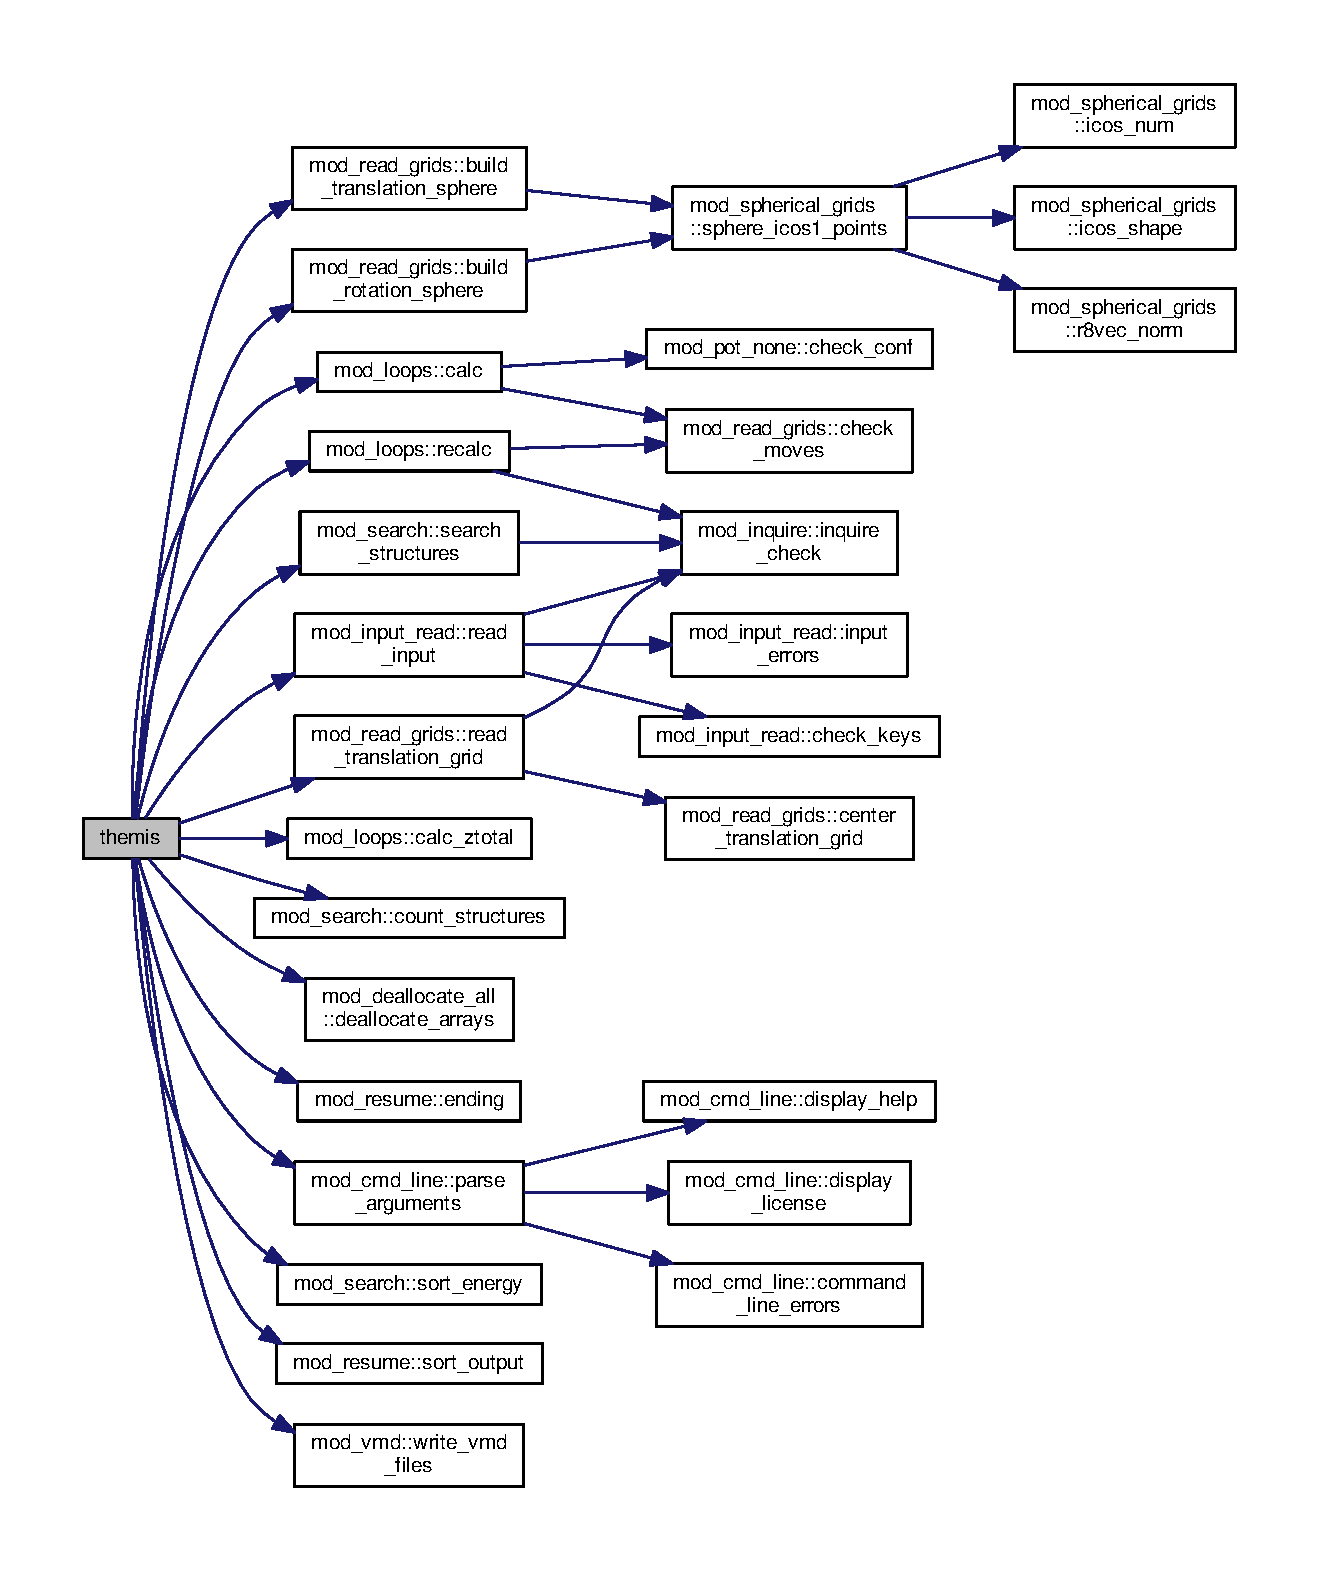
\includegraphics[width=350pt]{themis_8f90_a9fc0d5fc4c1bc4e9a810629a4d8cf52a_cgraph}
\end{center}
\end{figure}

\hypertarget{xdr_8f90}{}\section{/home/alozada/\+T\+H\+E\+M\+I\+S-\/\+D\+E\+V/themis-\/dev/code/src/xdr.f90 File Reference}
\label{xdr_8f90}\index{/home/alozada/\+T\+H\+E\+M\+I\+S-\/\+D\+E\+V/themis-\/dev/code/src/xdr.\+f90@{/home/alozada/\+T\+H\+E\+M\+I\+S-\/\+D\+E\+V/themis-\/dev/code/src/xdr.\+f90}}
\subsection*{Data Types}
\begin{DoxyCompactItemize}
\item 
type \hyperlink{structxdr_1_1xtcfile}{xdr\+::xtcfile}
\end{DoxyCompactItemize}
\subsection*{Modules}
\begin{DoxyCompactItemize}
\item 
module \hyperlink{namespacexdr}{xdr}
\begin{DoxyCompactList}\small\item\em X\+DR Fortran Interface with Wrappers. \end{DoxyCompactList}\end{DoxyCompactItemize}

\hypertarget{mainpage_8dox}{}\section{mainpage.\+dox File Reference}
\label{mainpage_8dox}\index{mainpage.\+dox@{mainpage.\+dox}}

%--- End generated contents ---

% Index
\backmatter
\newpage
\phantomsection
\clearemptydoublepage
\addcontentsline{toc}{chapter}{Index}
\printindex

\end{document}
